% Created 2021-06-26 Sat 23:42
% Intended LaTeX compiler: pdflatex
\documentclass[11pt]{article}
\usepackage[utf8]{inputenc}
\usepackage[T1]{fontenc}
\usepackage{graphicx}
\usepackage{grffile}
\usepackage{longtable}
\usepackage{wrapfig}
\usepackage{rotating}
\usepackage[normalem]{ulem}
\usepackage{amsmath}
\usepackage{textcomp}
\usepackage{amssymb}
\usepackage{capt-of}
\usepackage{hyperref}
\usepackage[utf8x]{inputenc}
\usepackage[T2A]{fontenc}
\hypersetup{colorlinks, citecolor=black, filecolor=black, linkcolor=black, urlcolor=black}
\usepackage[pdftex]{graphicx}
\usepackage{pdfpages}
\author{q}
\date{\today}
\title{Алгебра. Подготвка к экзамену.}
\hypersetup{
 pdfauthor={q},
 pdftitle={Алгебра. Подготвка к экзамену.},
 pdfkeywords={},
 pdfsubject={},
 pdfcreator={Emacs 27.2 (Org mode 9.4.4)}, 
 pdflang={English}}
\begin{document}

\maketitle
\tableofcontents


\section{«Алгебра, часть II»}
\label{sec:orge8841ff}
\subsection{1.Кольцо многочленов R[x] над областью целостности R. Теорема Безу. Теорема о числе корней многочлена. Формулы Виета.}
\label{sec:org58b308d}
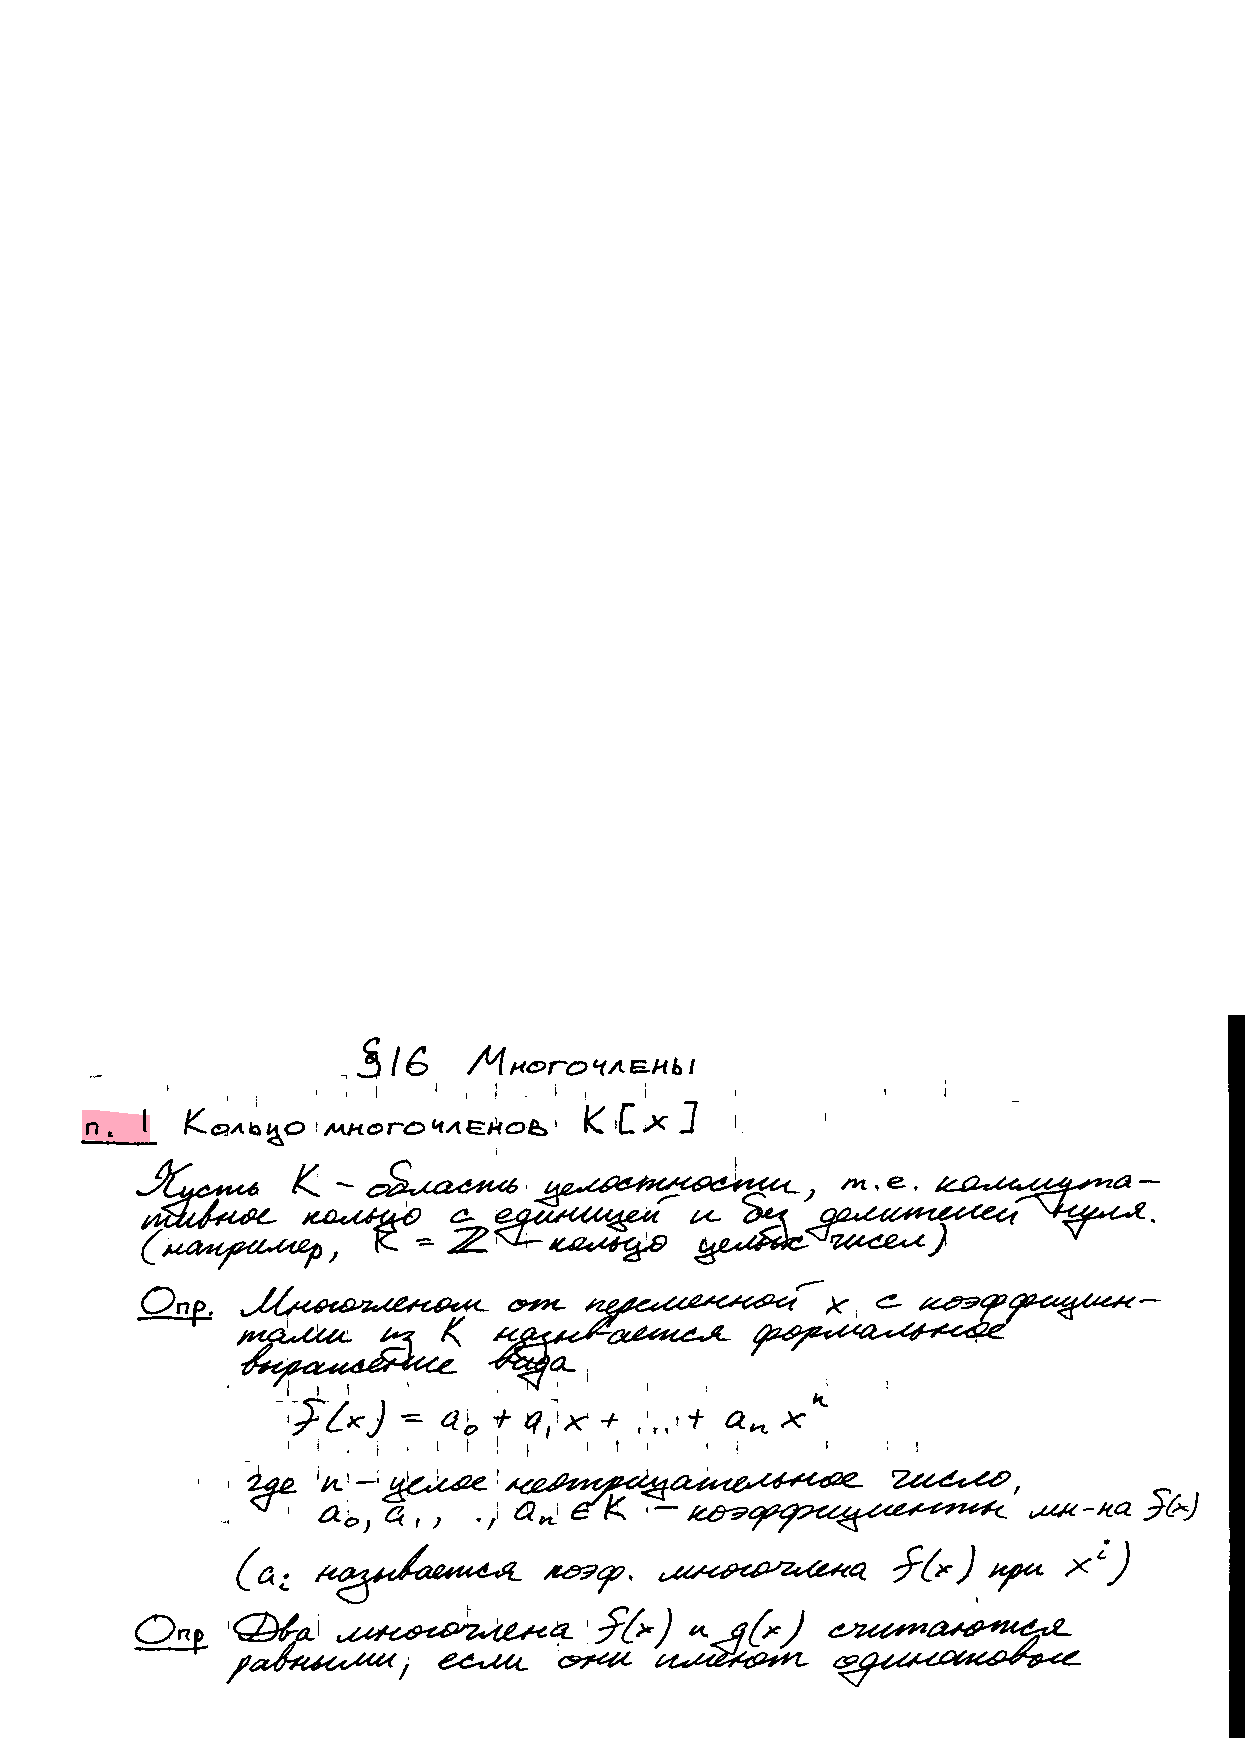
\includepdf[pages=-]{pdf/1_1.pdf}

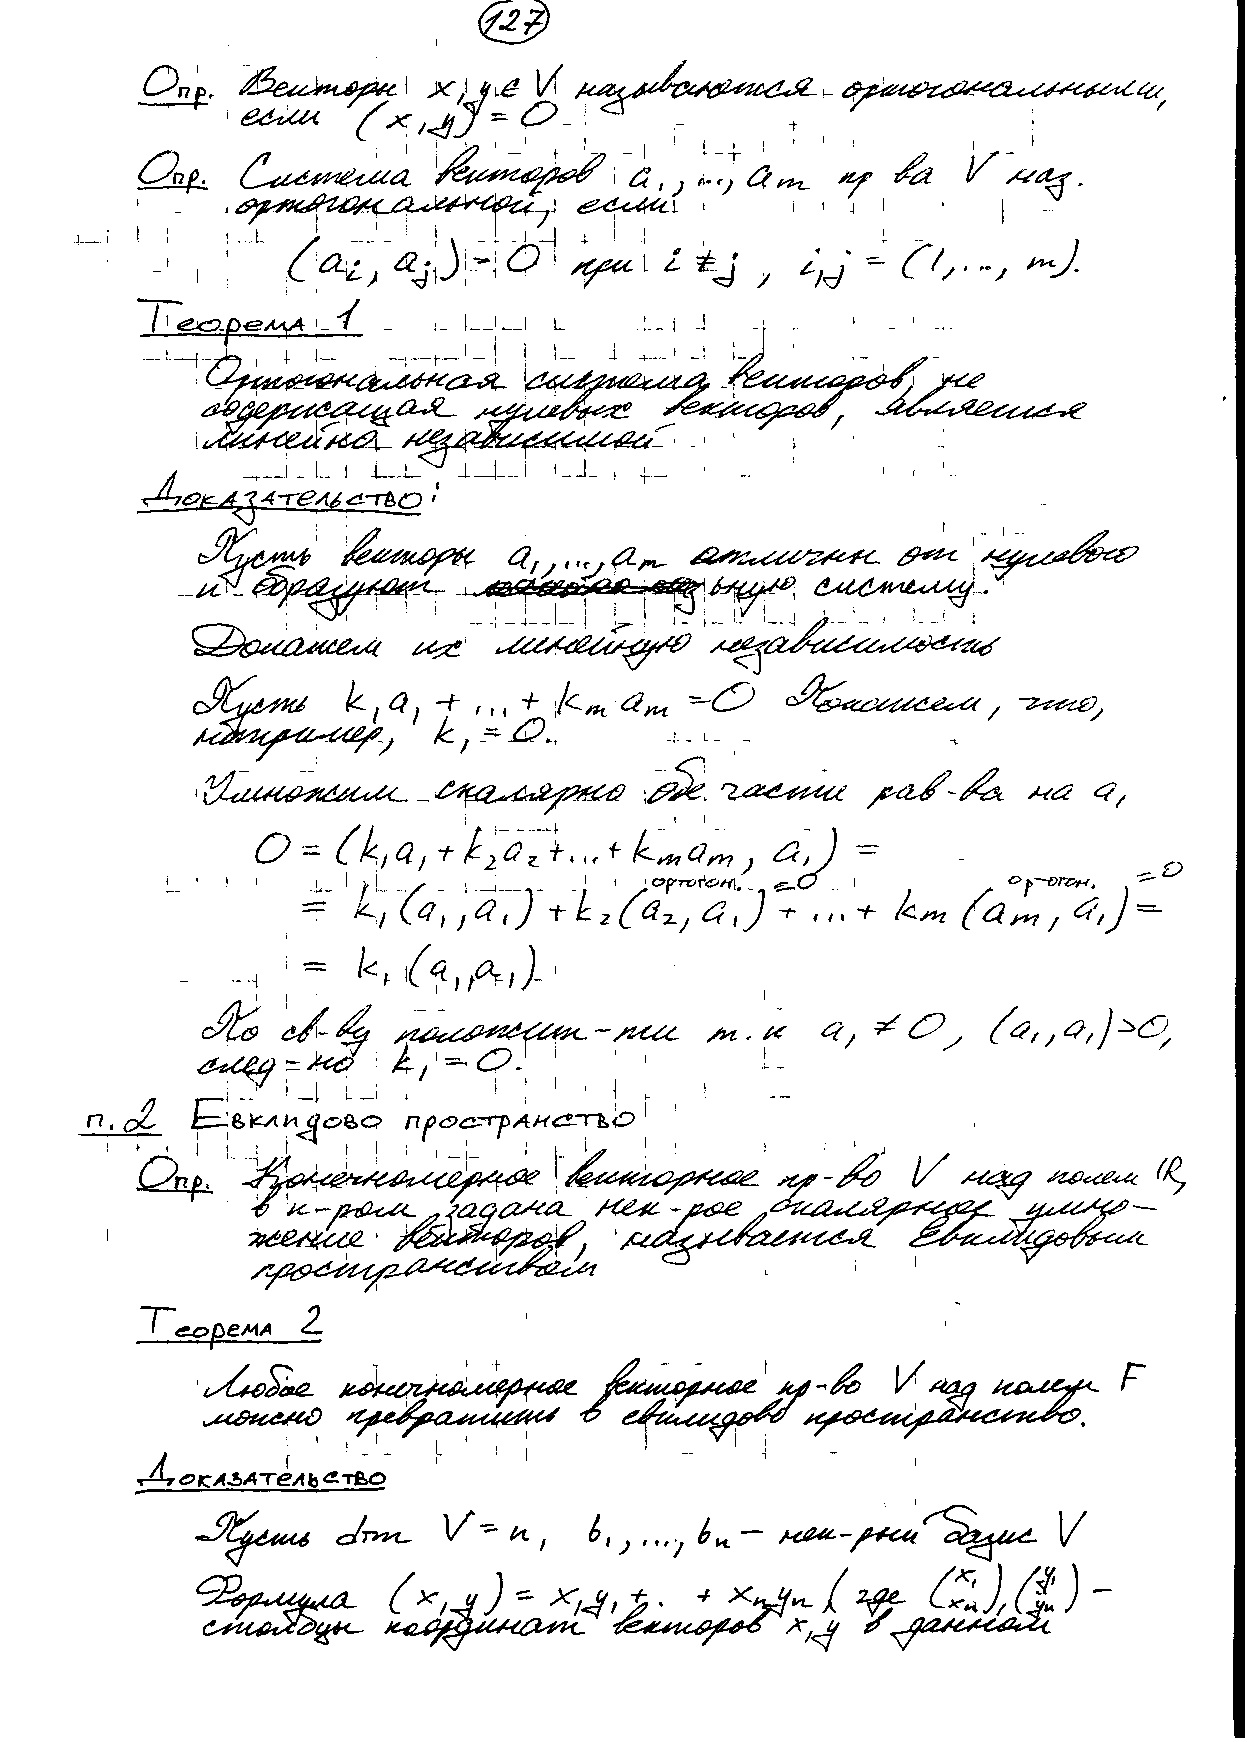
\includepdf[pages=-]{pdf/1_2.pdf}

\subsection{2. Алгебраическое и функциональное равенство многочленов. Интерполяционная формула Лагранжа.}
\label{sec:orgcf976fc}
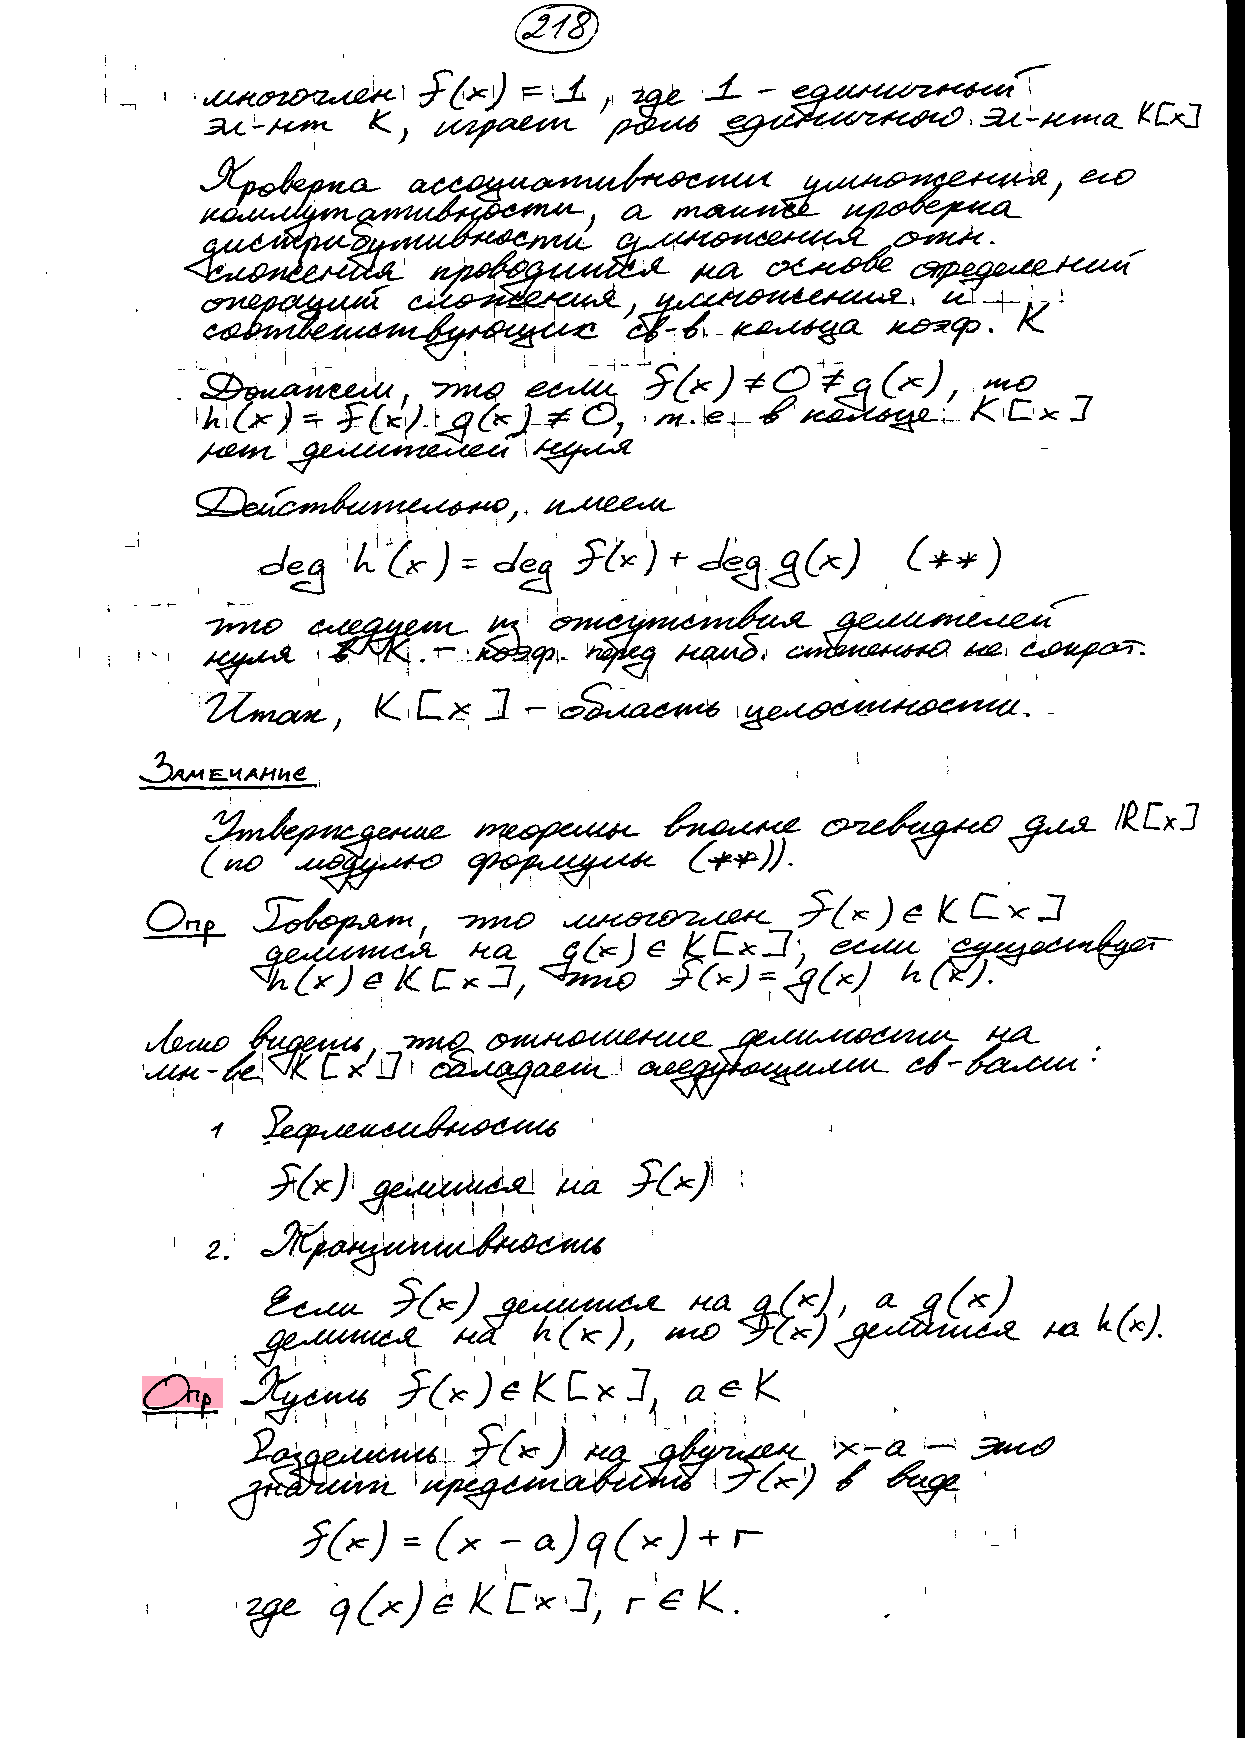
\includepdf[pages=-]{pdf/2_1.pdf}

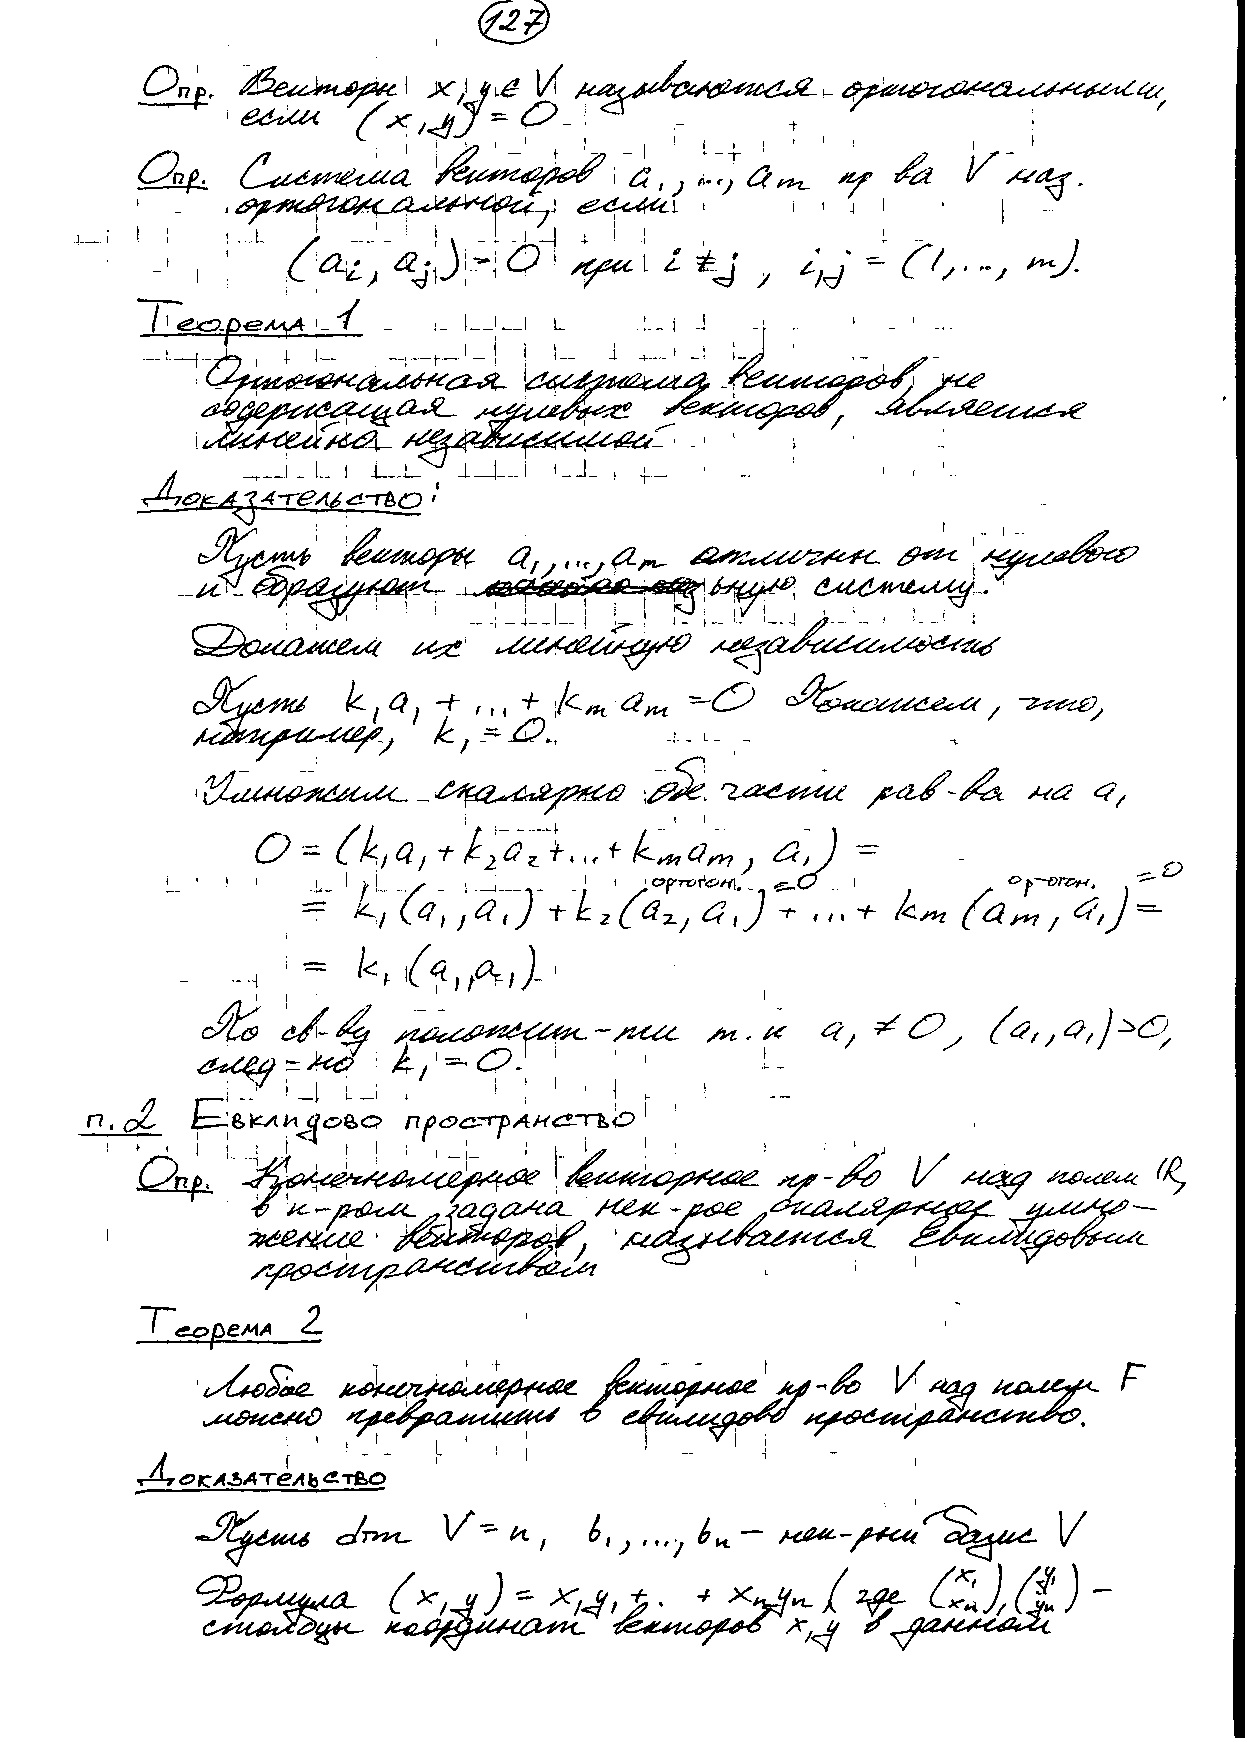
\includepdf[pages=-]{pdf/2_2.pdf}

\subsection{3. Кольцо многочленов F[x] над полем F. Деление с остатком. Наибольший общий делитель многочленов.}
\label{sec:orga29fa8b}
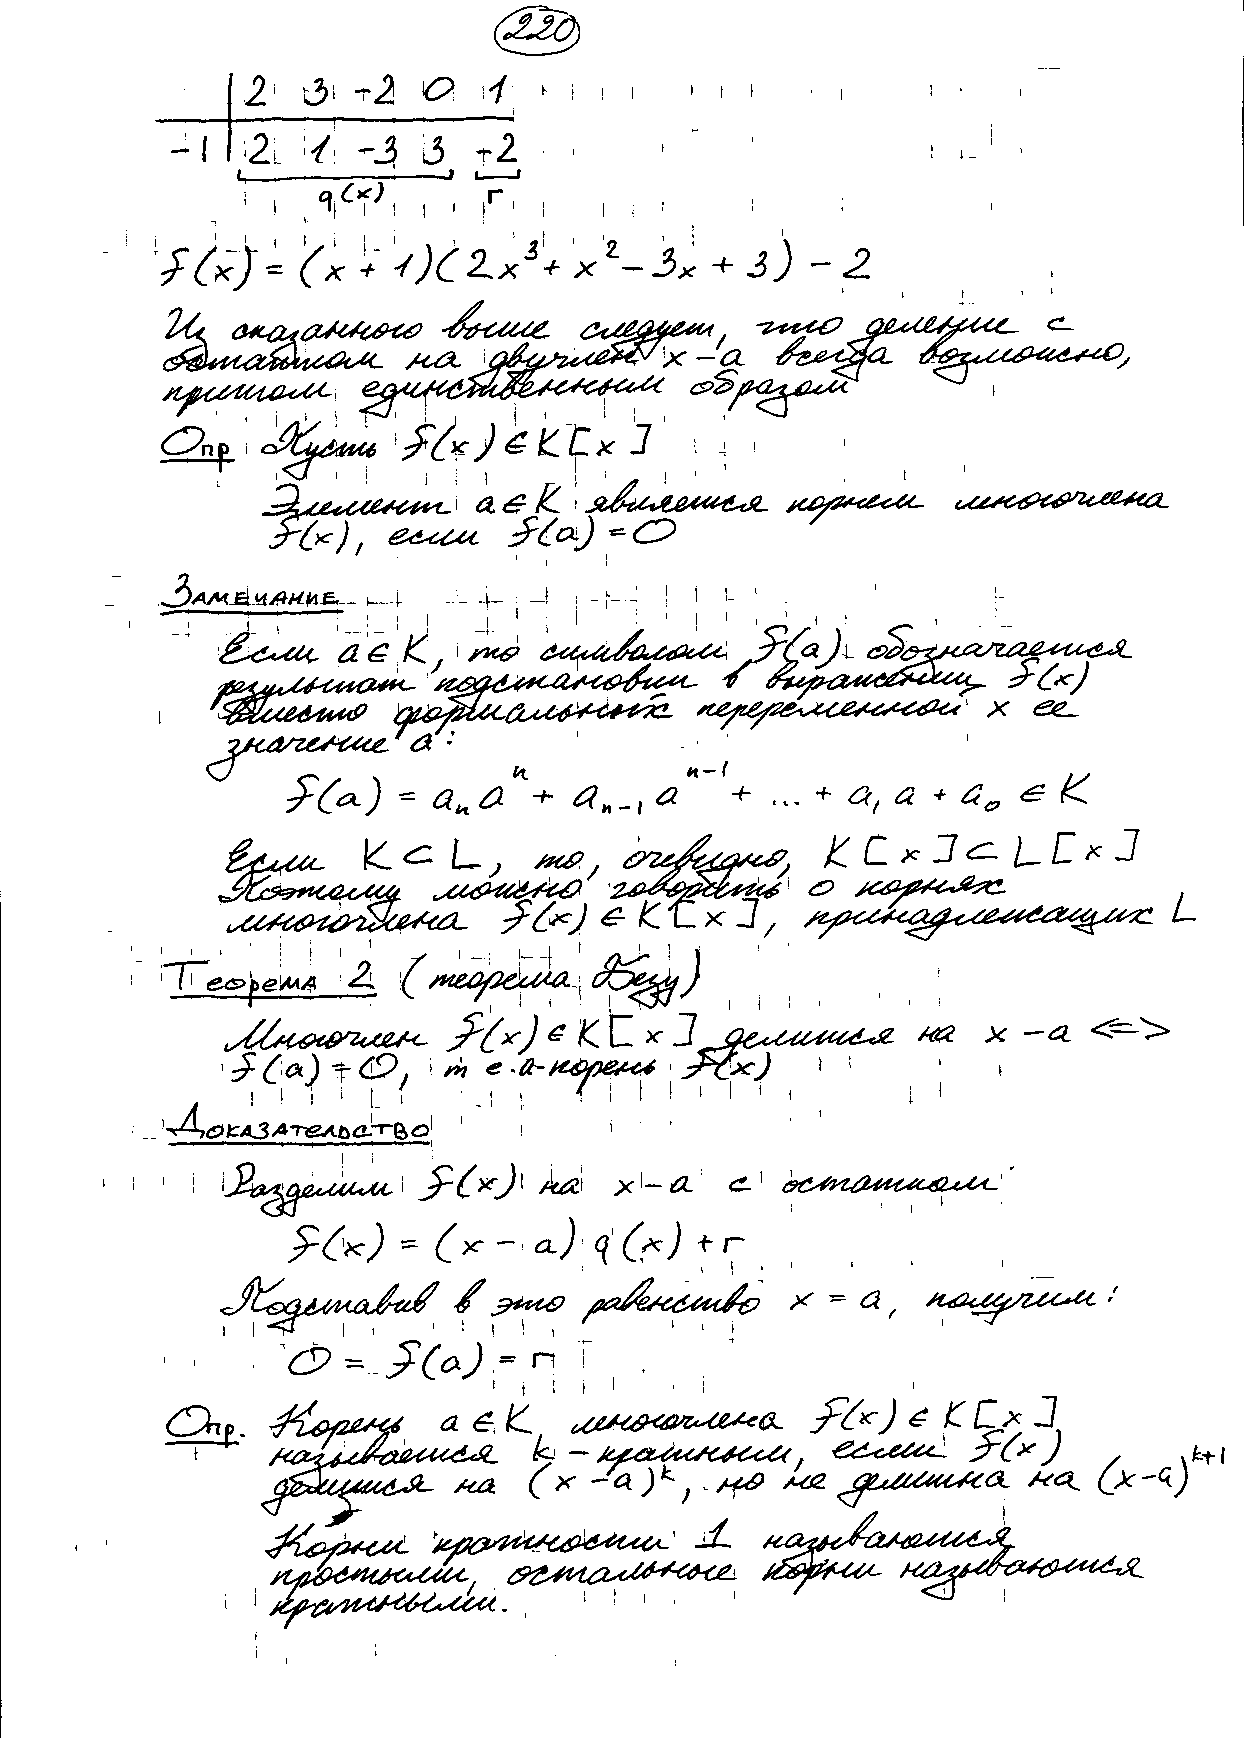
\includepdf[pages=-]{pdf/3_1.pdf}

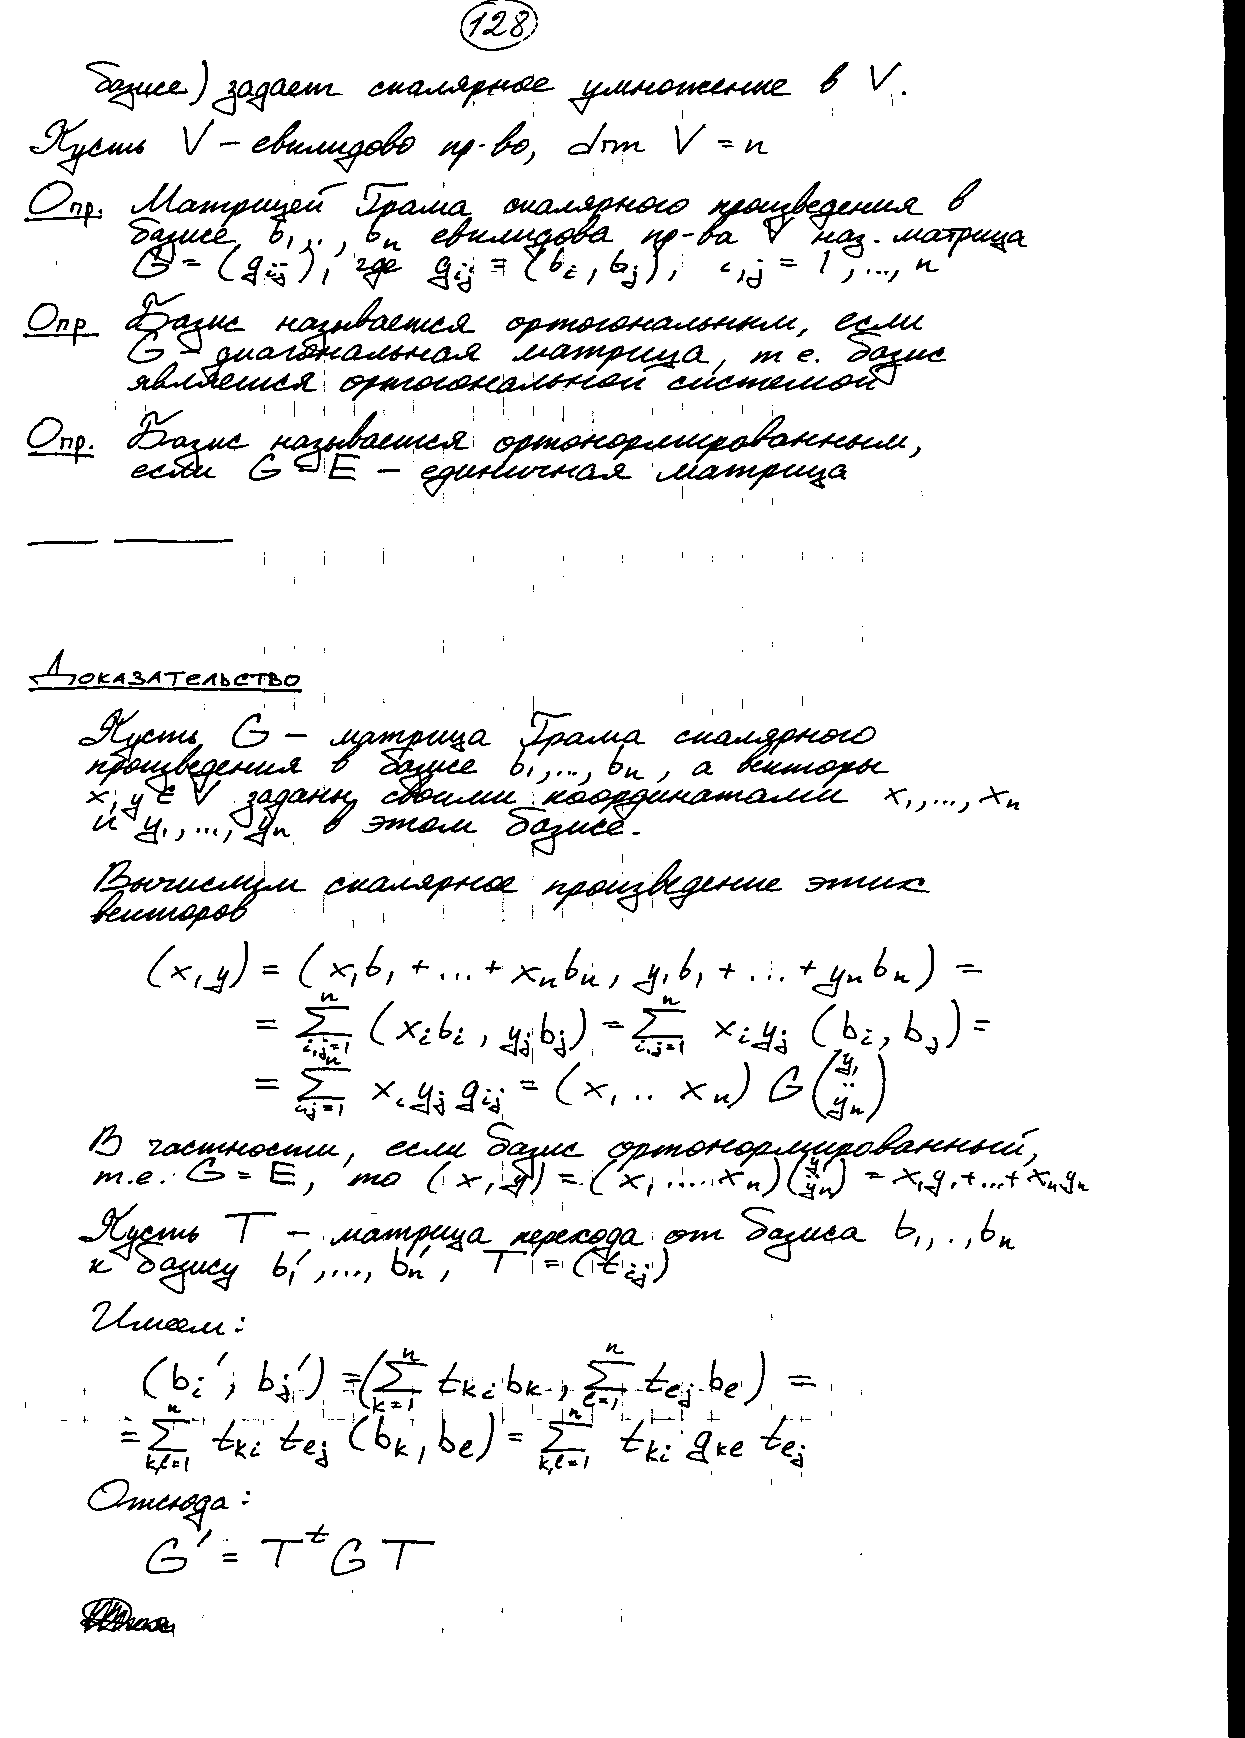
\includepdf[pages=-]{pdf/3_2.pdf}

\subsection{4. Алгоритм Евклида. Линейная форма наибольшего общего делителя многочленов.}
\label{sec:orge148261}
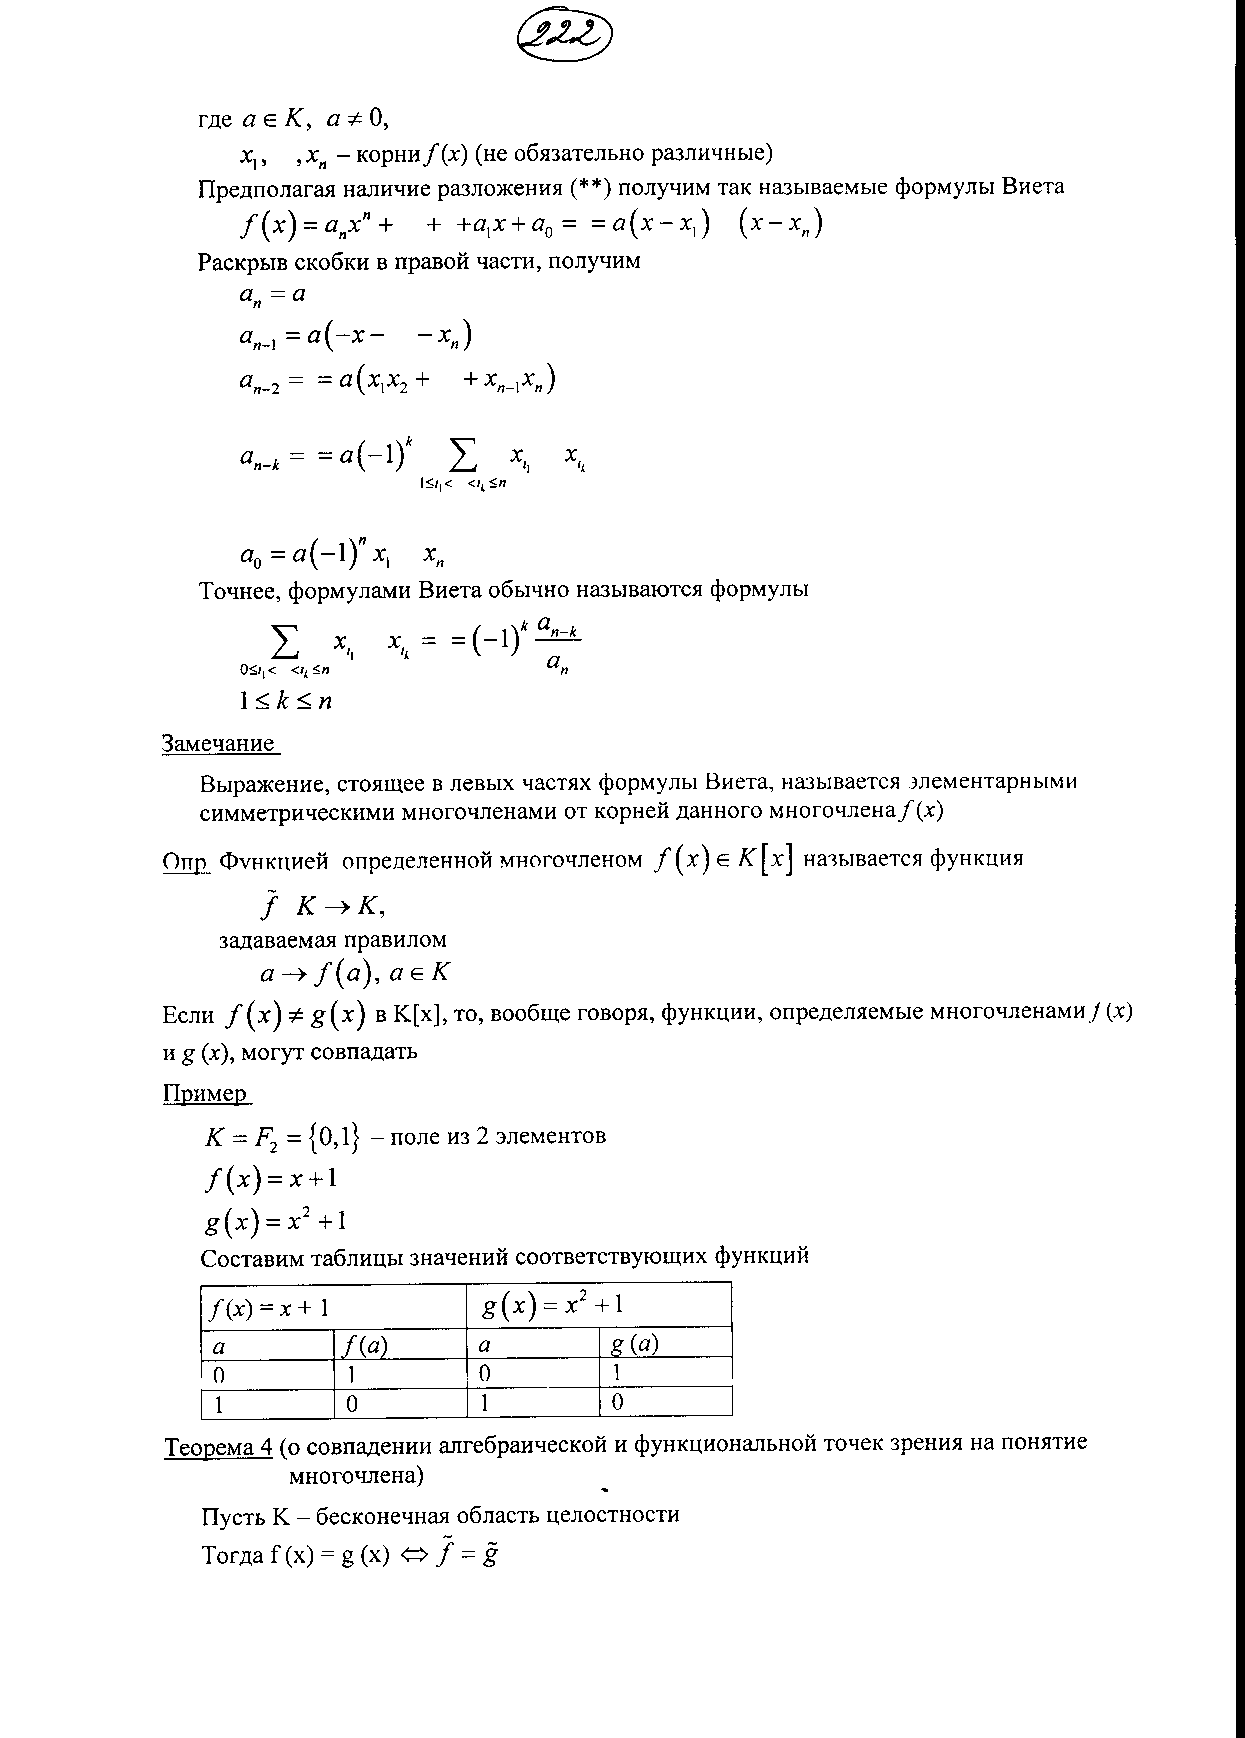
\includepdf[pages=-]{pdf/4_1.pdf}

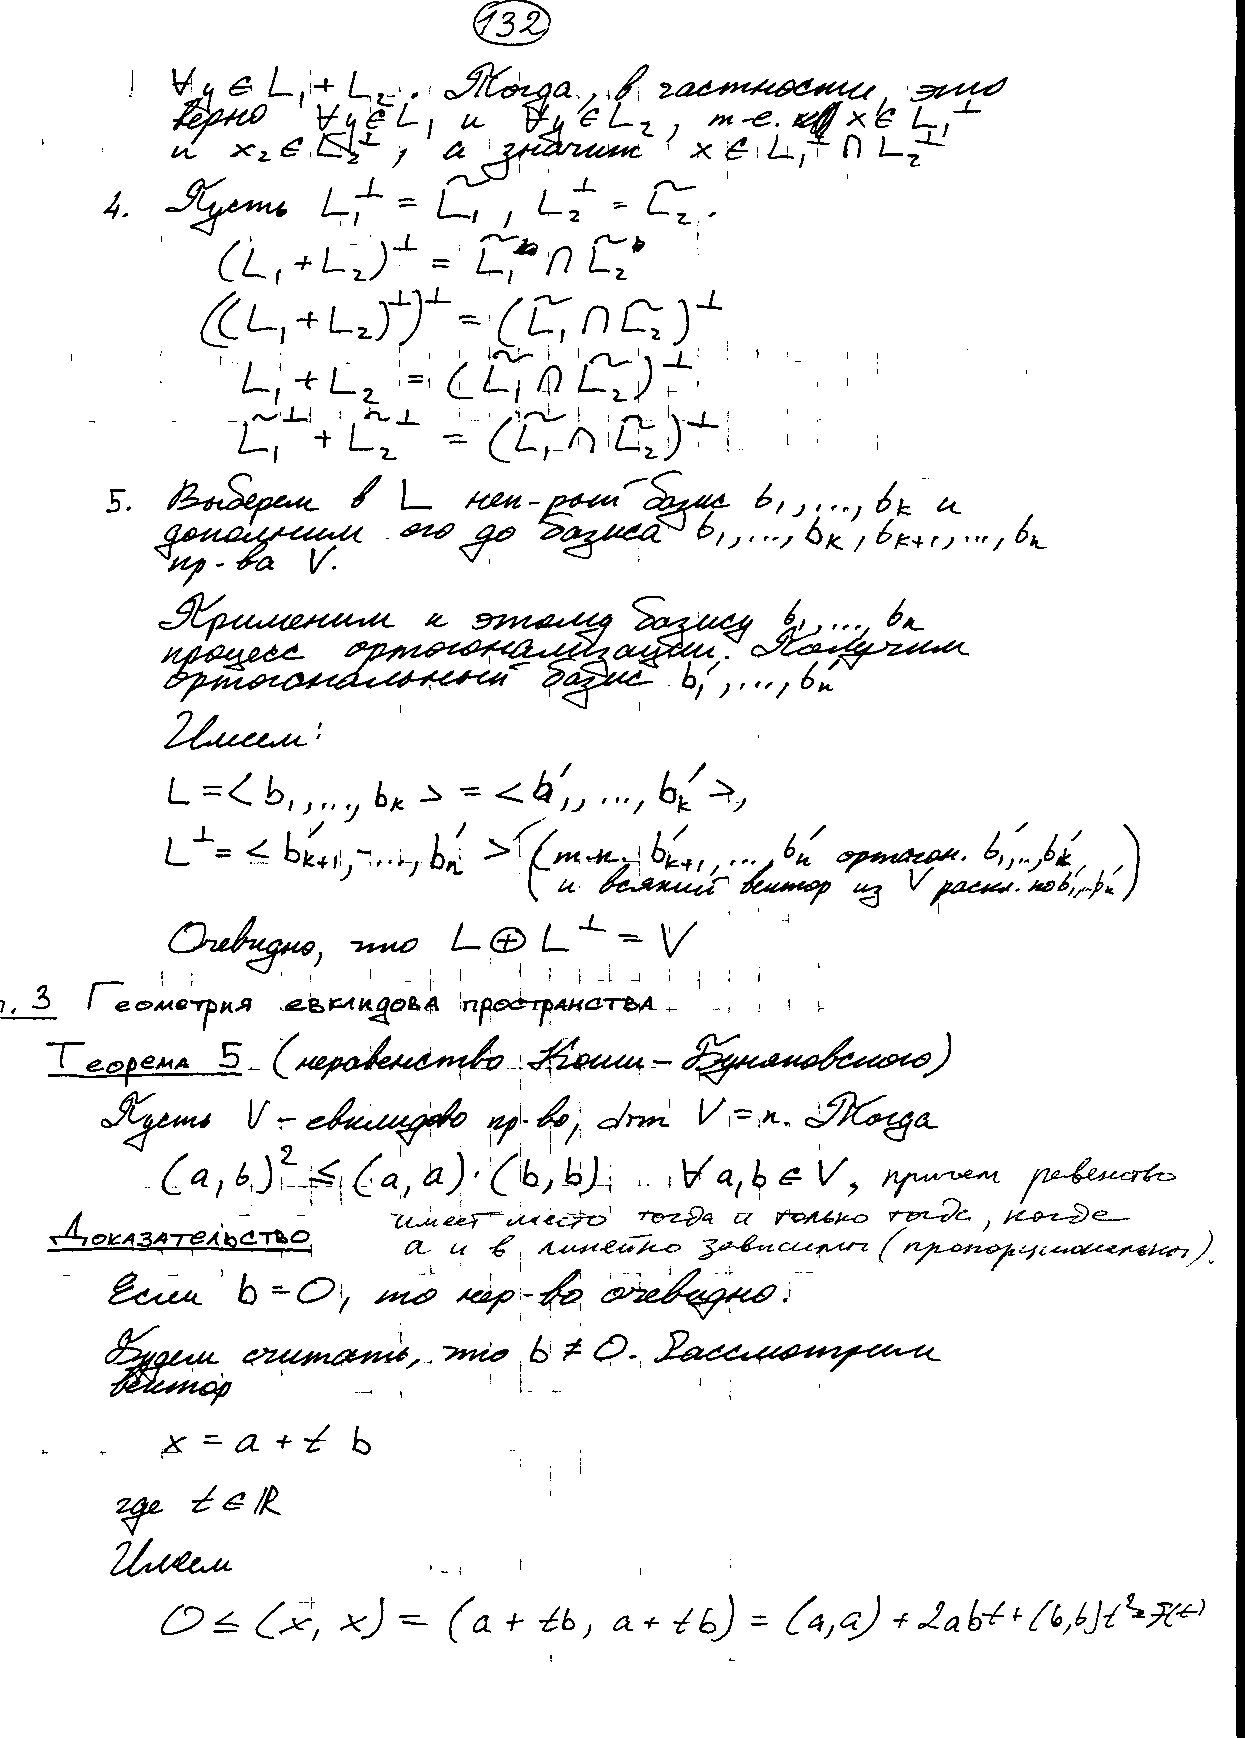
\includepdf[pages=-]{pdf/4_2.pdf}

\subsection{2. Взаимно простые многочлены и их свойства. Наименьшее общее кратное многочленов.}
\label{sec:org927d353}
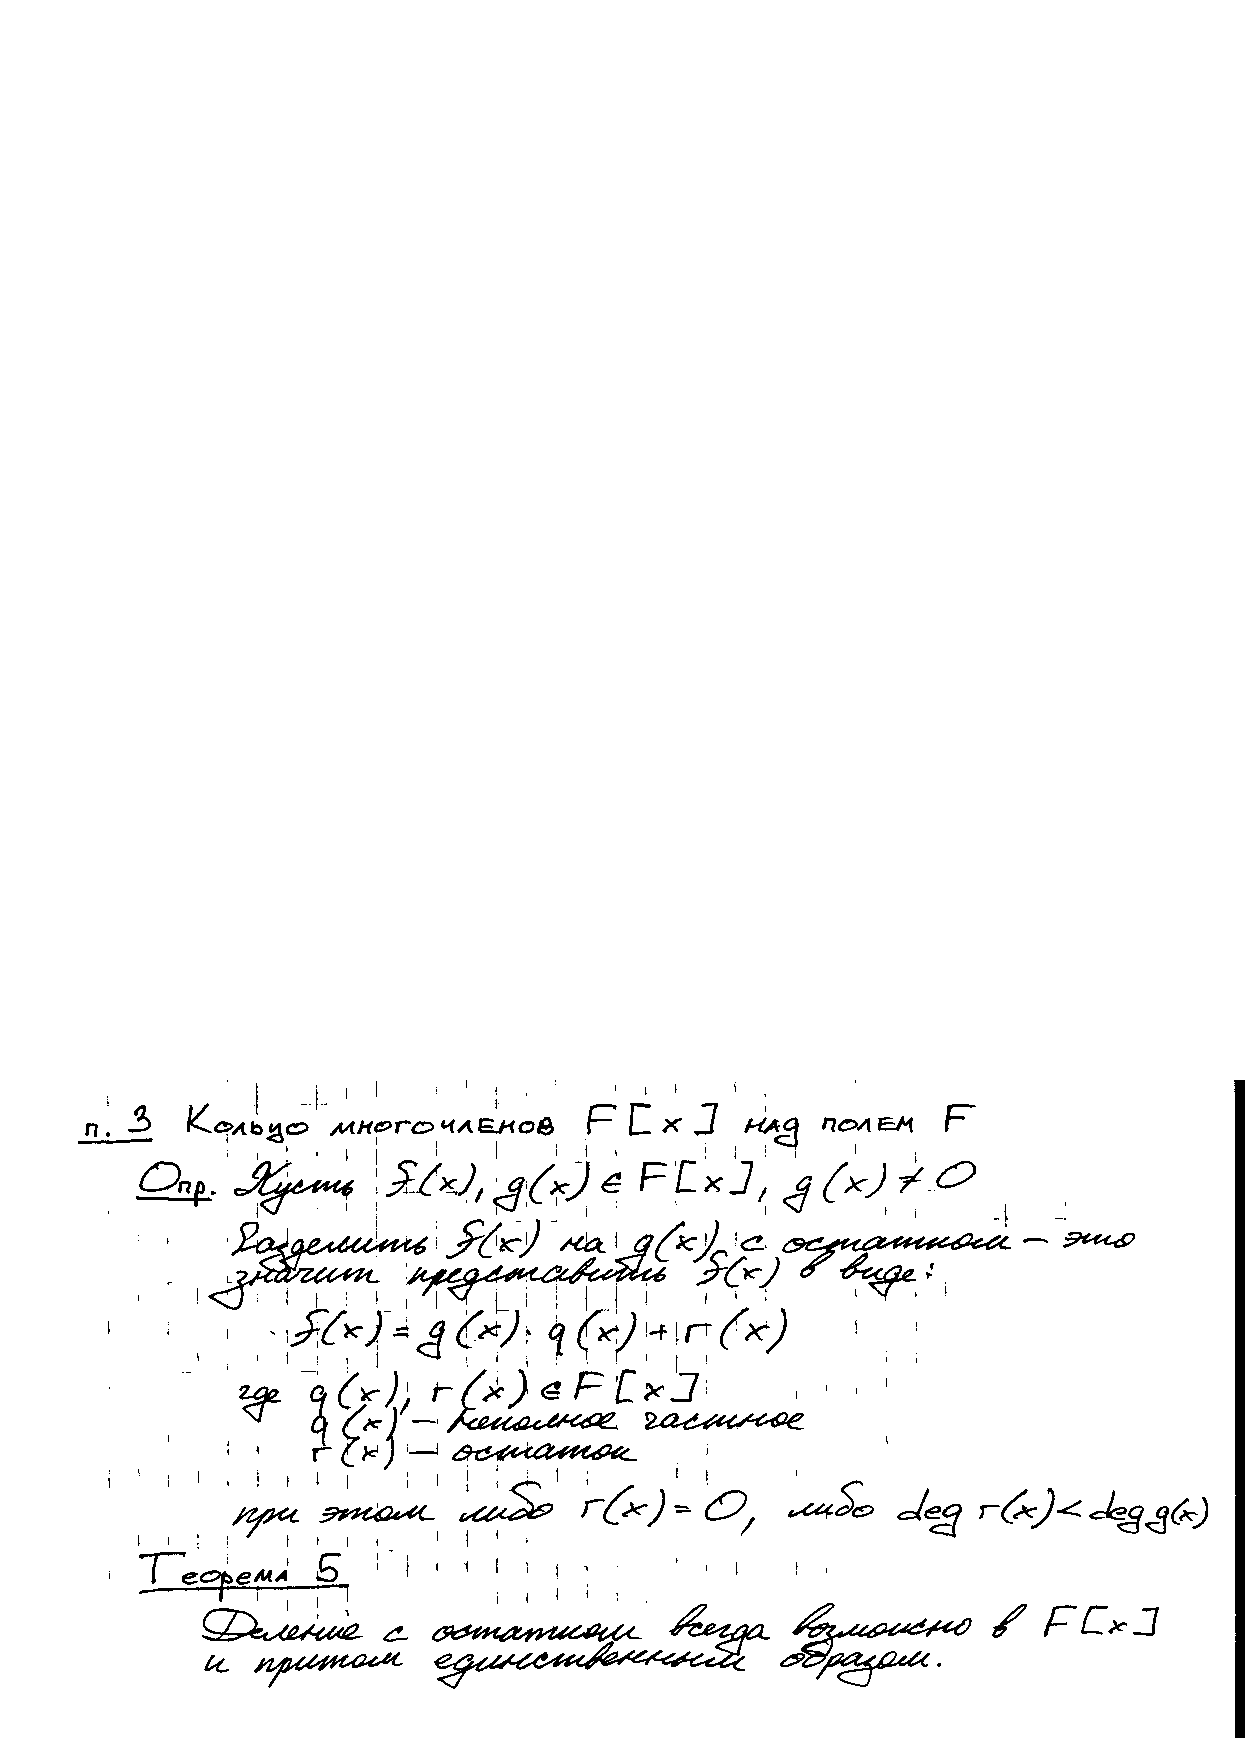
\includepdf[pages=-]{pdf/5_1.pdf}

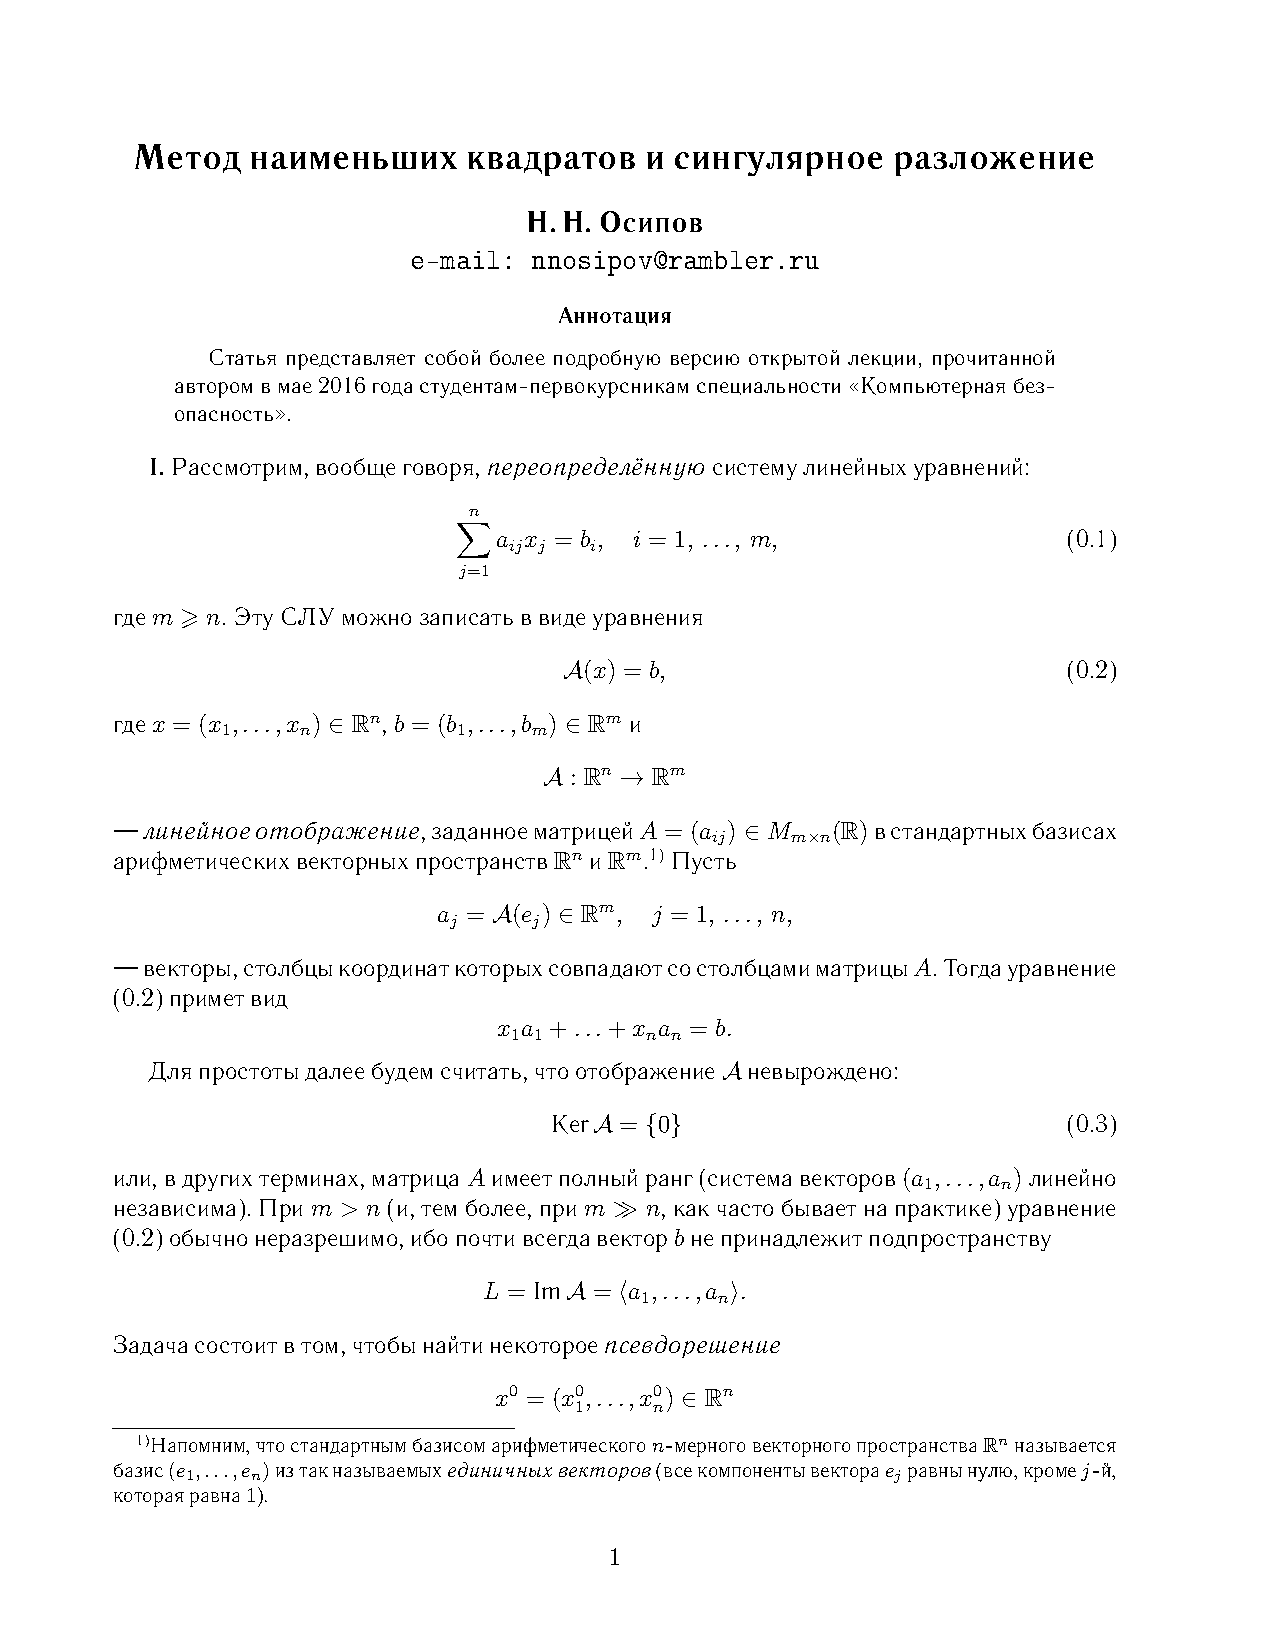
\includepdf[pages=-]{pdf/5_2.pdf}

\subsection{3. Неприводимые многочлены над полем. Теорема о факторизации.}
\label{sec:org400287e}
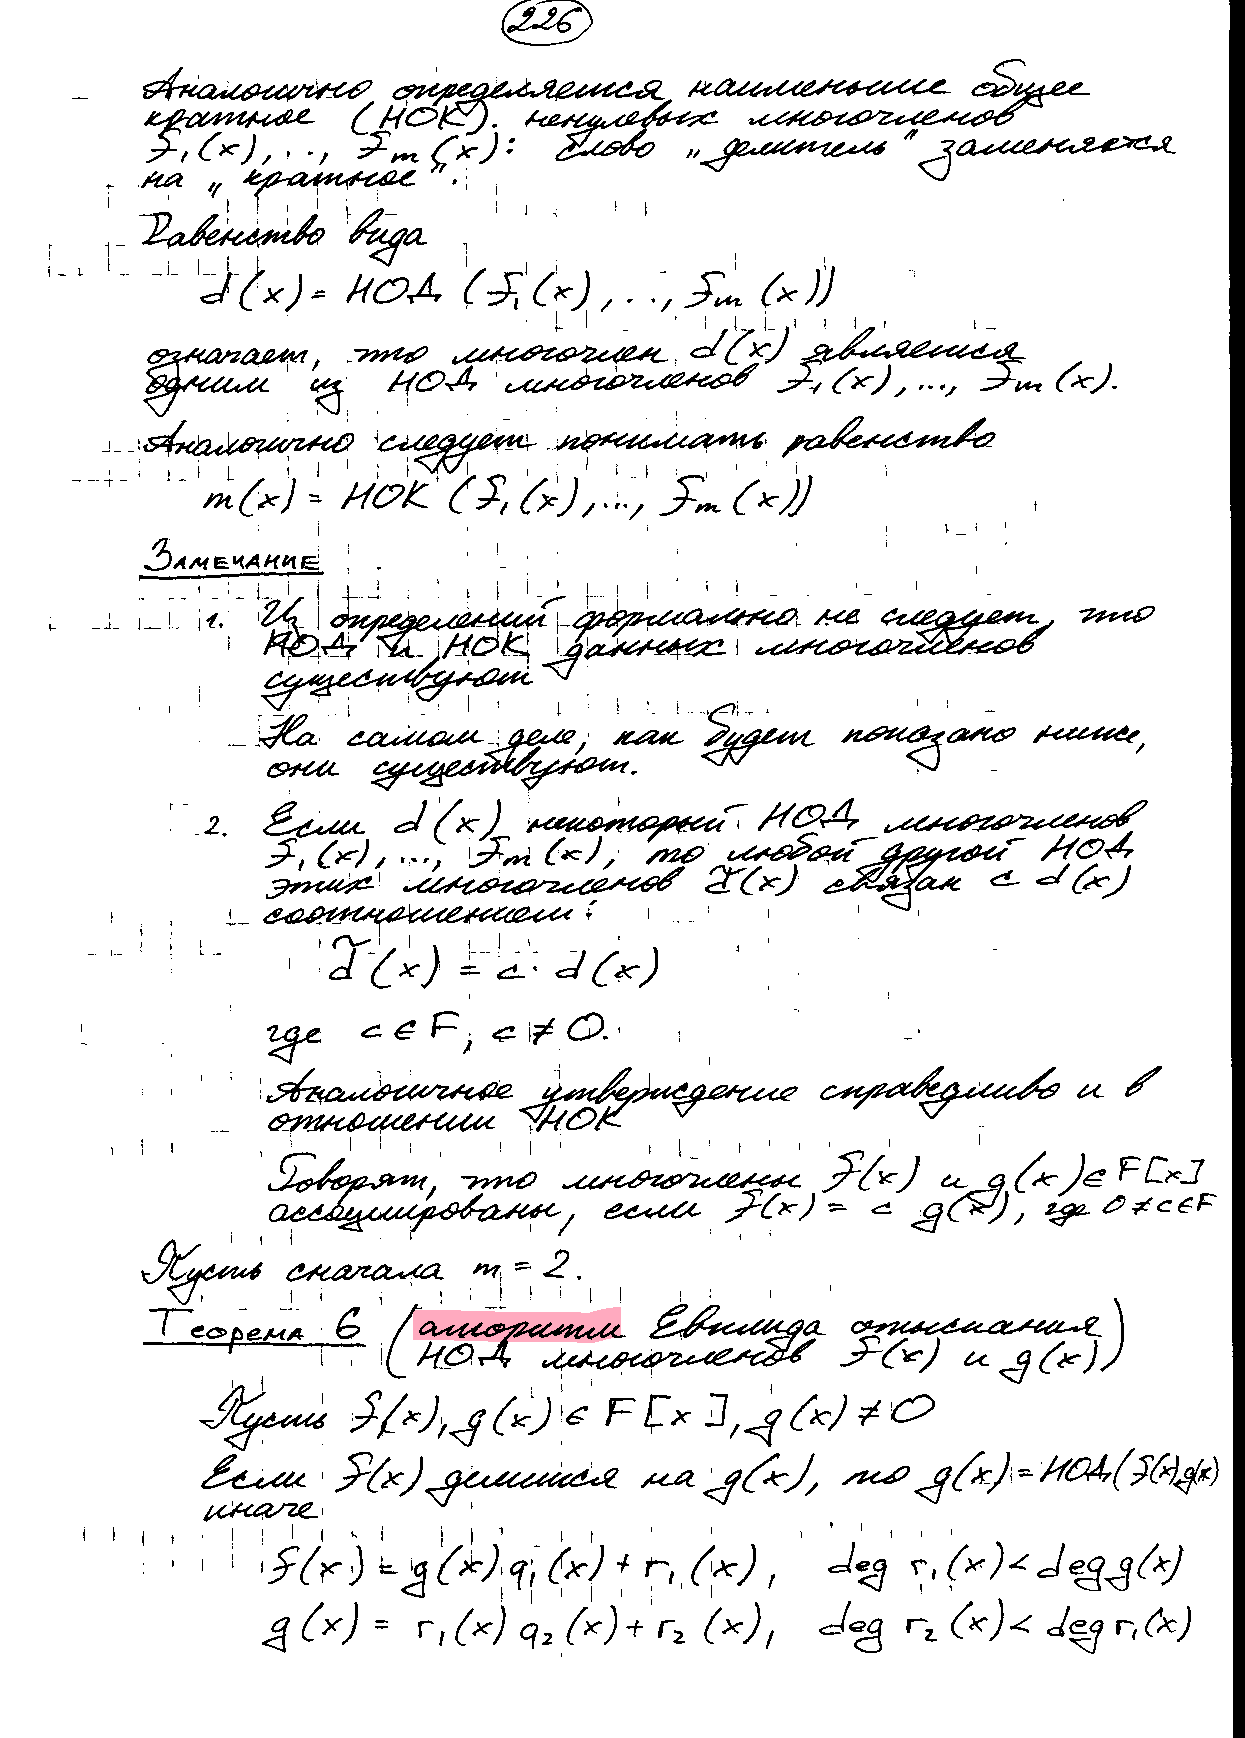
\includepdf[pages=-]{pdf/6_1.pdf}

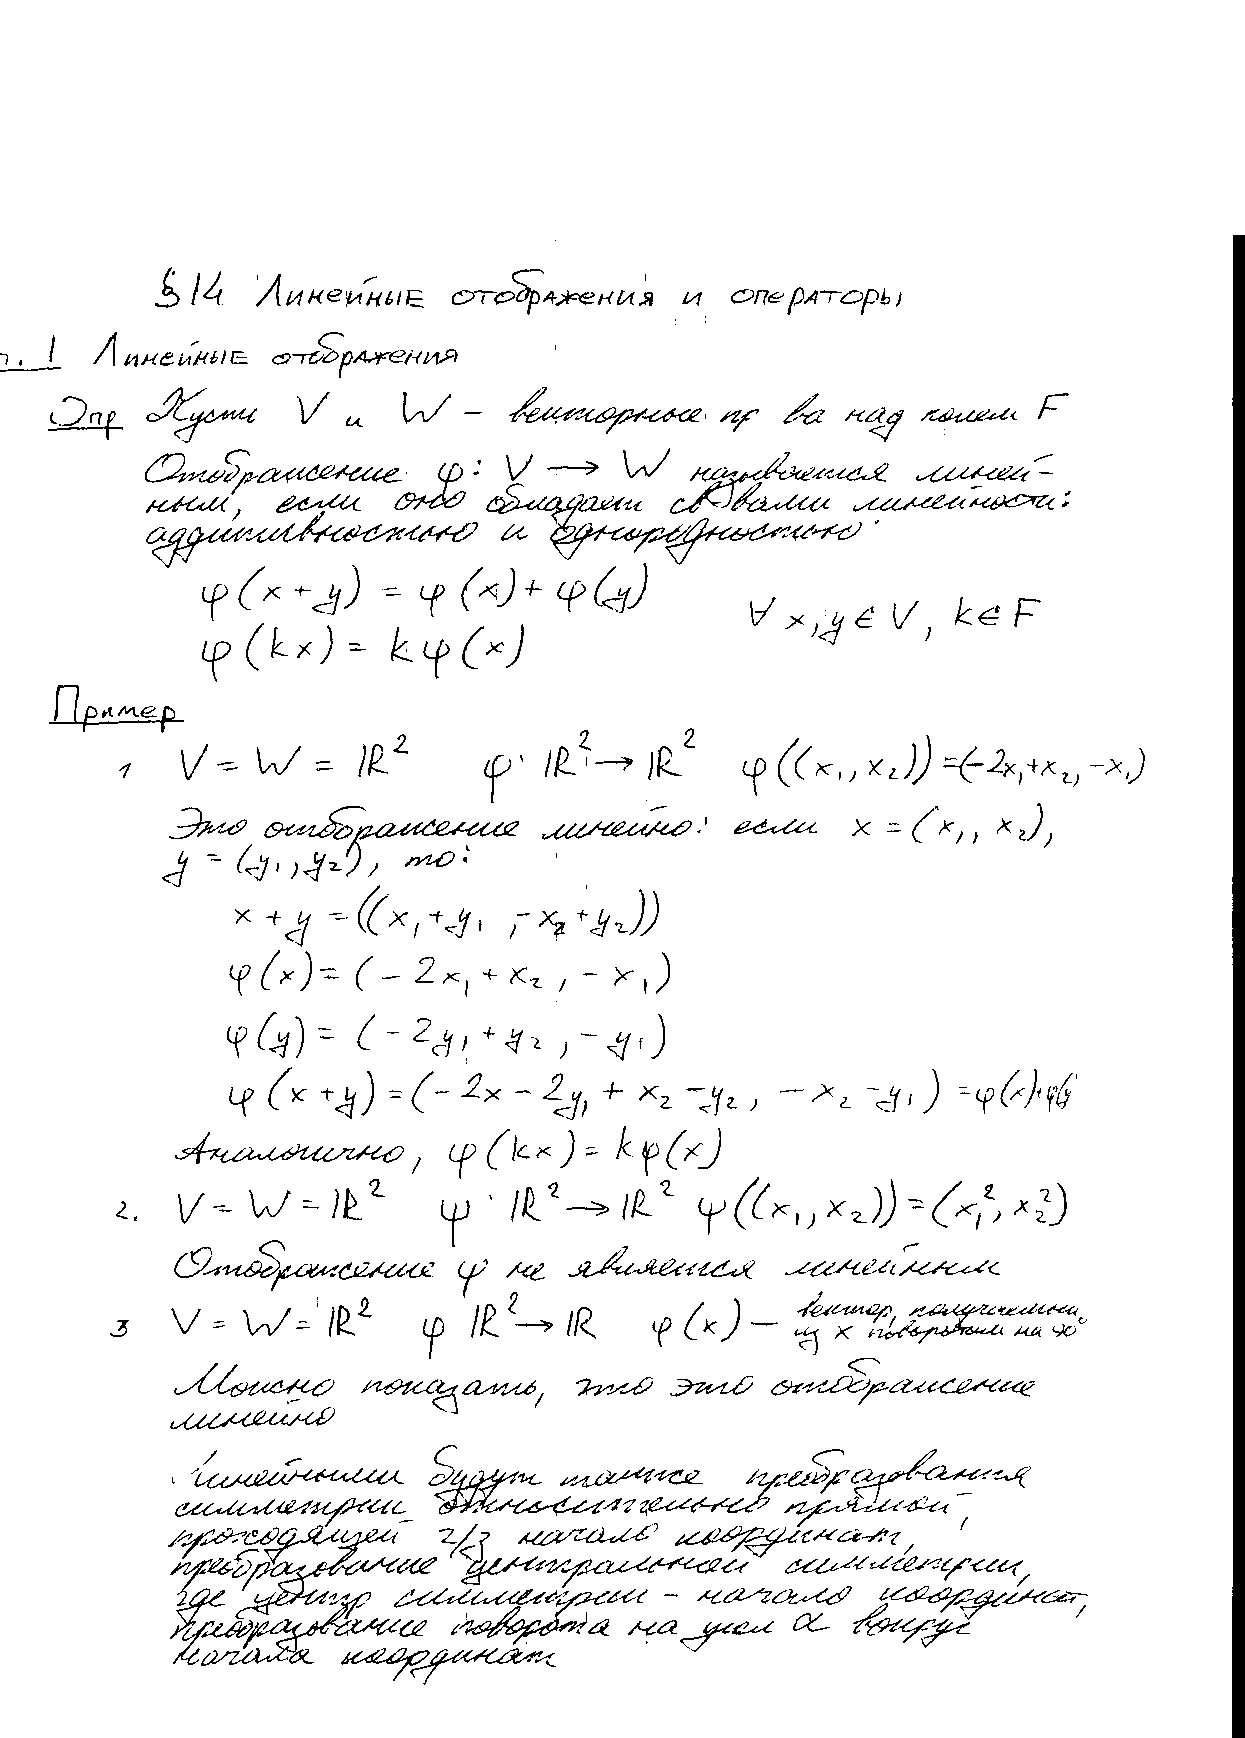
\includepdf[pages=-]{pdf/6_2.pdf}

\subsection{4. Многочлены над C и R. Основная теорема алгебры многочленов и её следствия. Многочлены над Q. Критерий Эйзенштейна неприводимости многочлена над Q.}
\label{sec:orgfcc45a8}
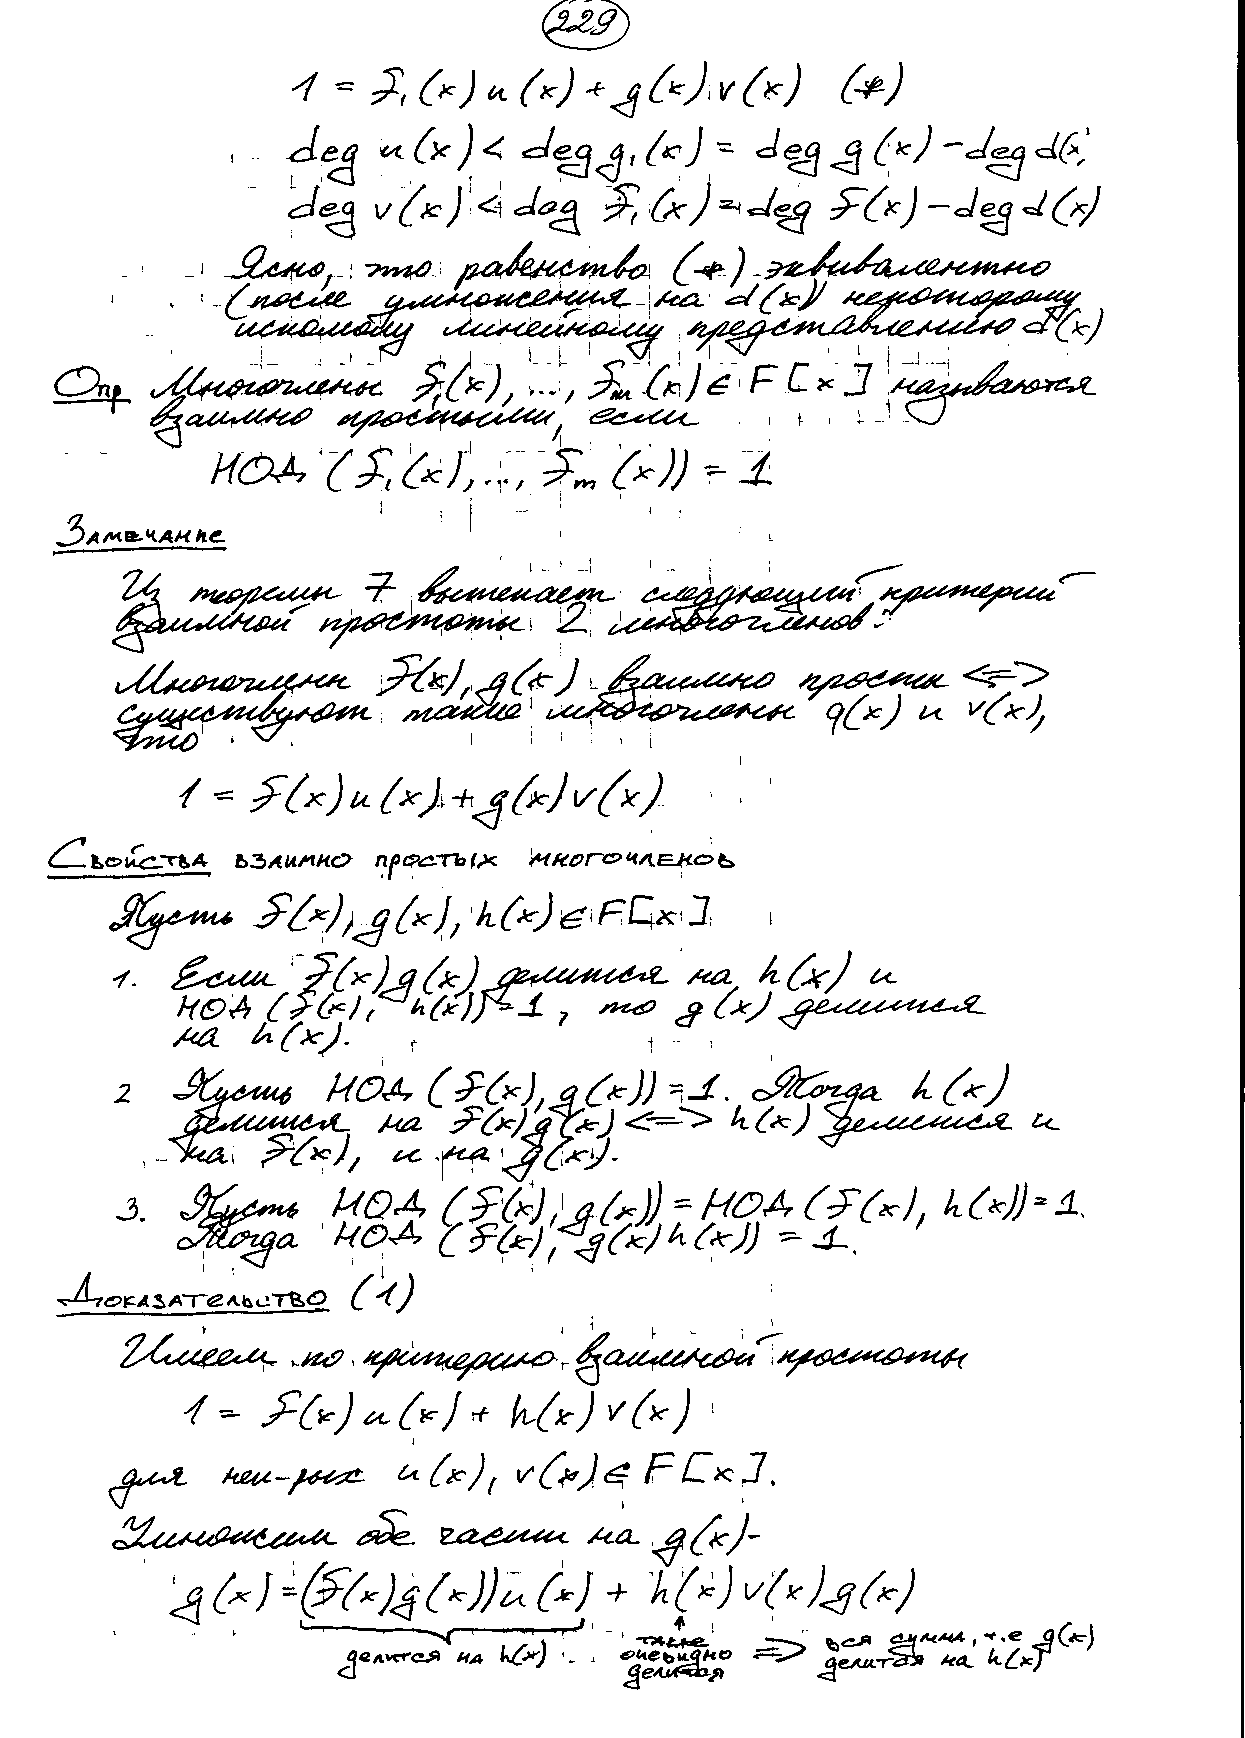
\includepdf[pages=-]{pdf/7_1.pdf}

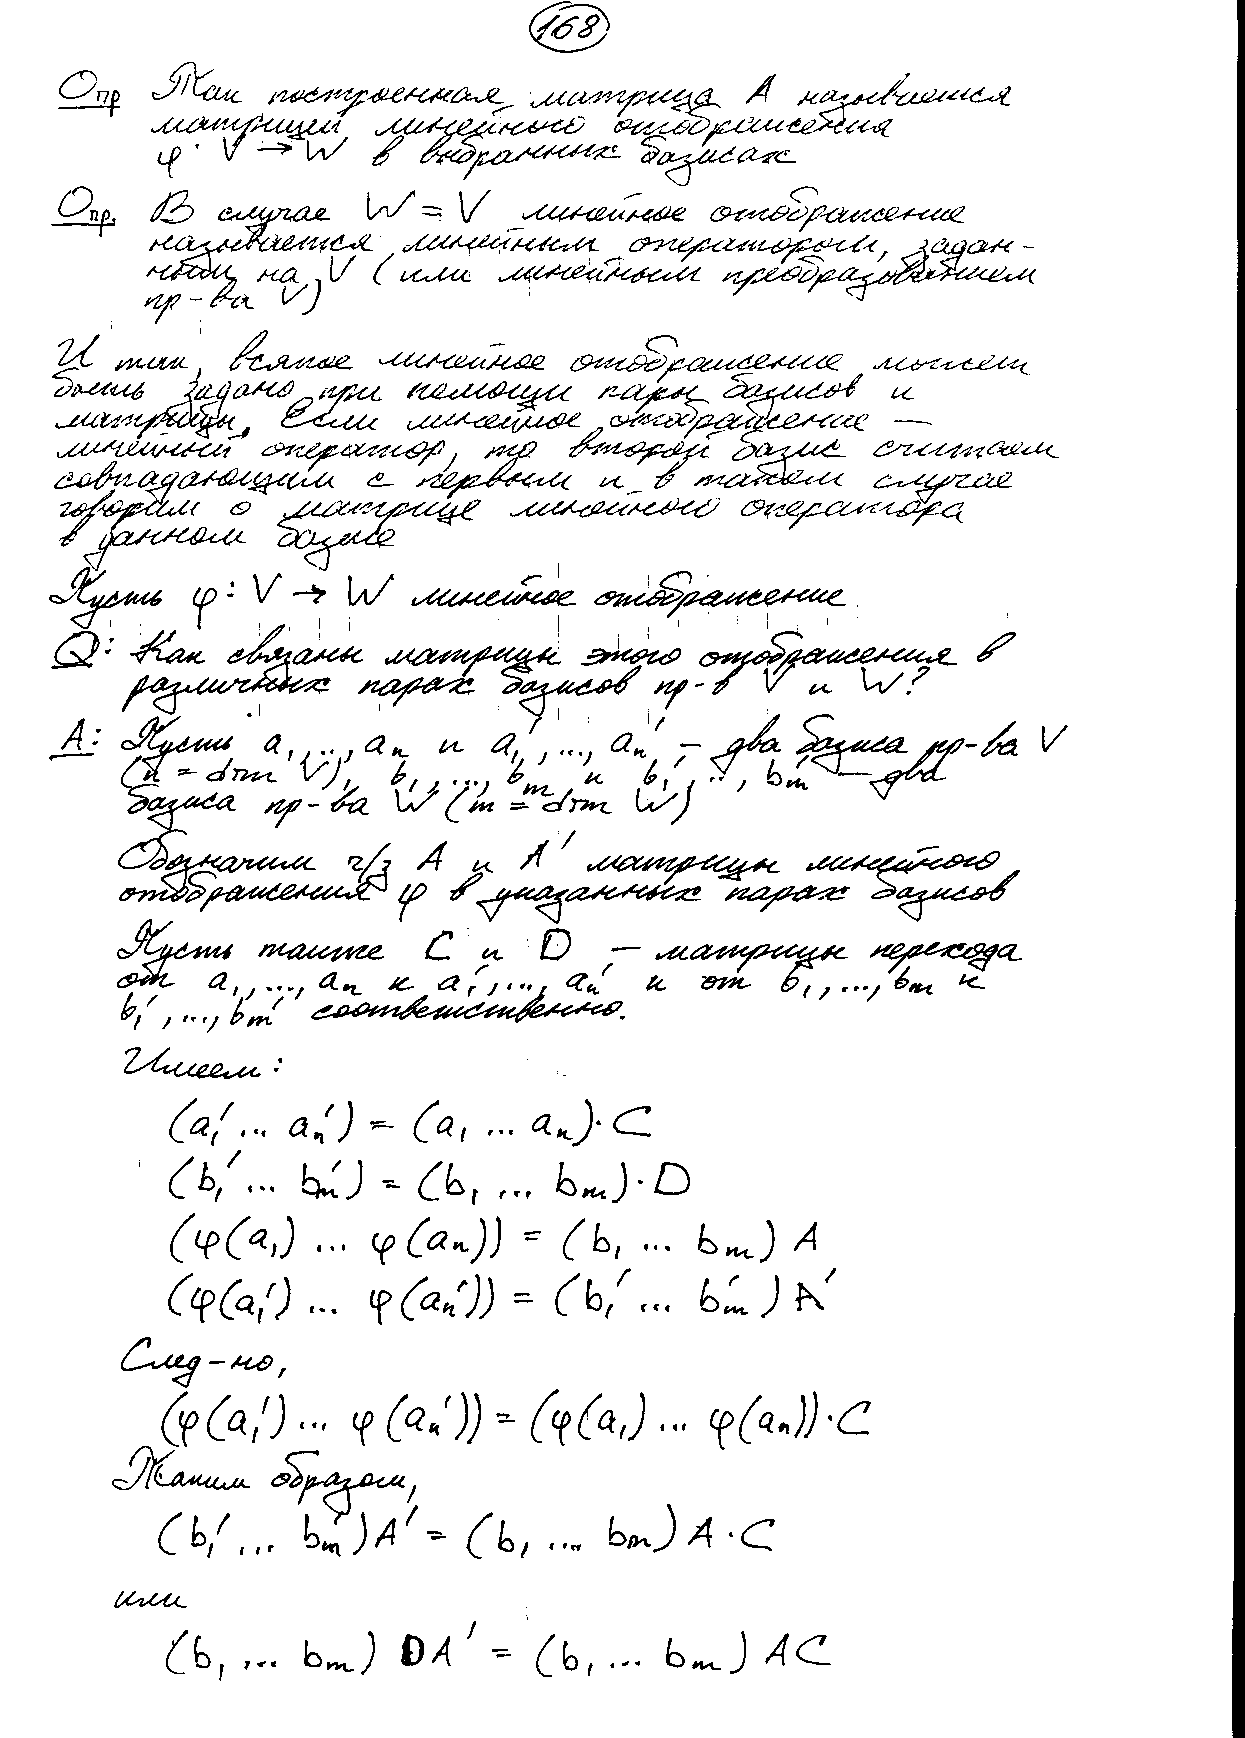
\includepdf[pages=-]{pdf/7_2.pdf}

\subsection{5. Векторное пространство над полем скаляров. Подпространство, характеристический признак подпространства.}
\label{sec:orga02cdc6}
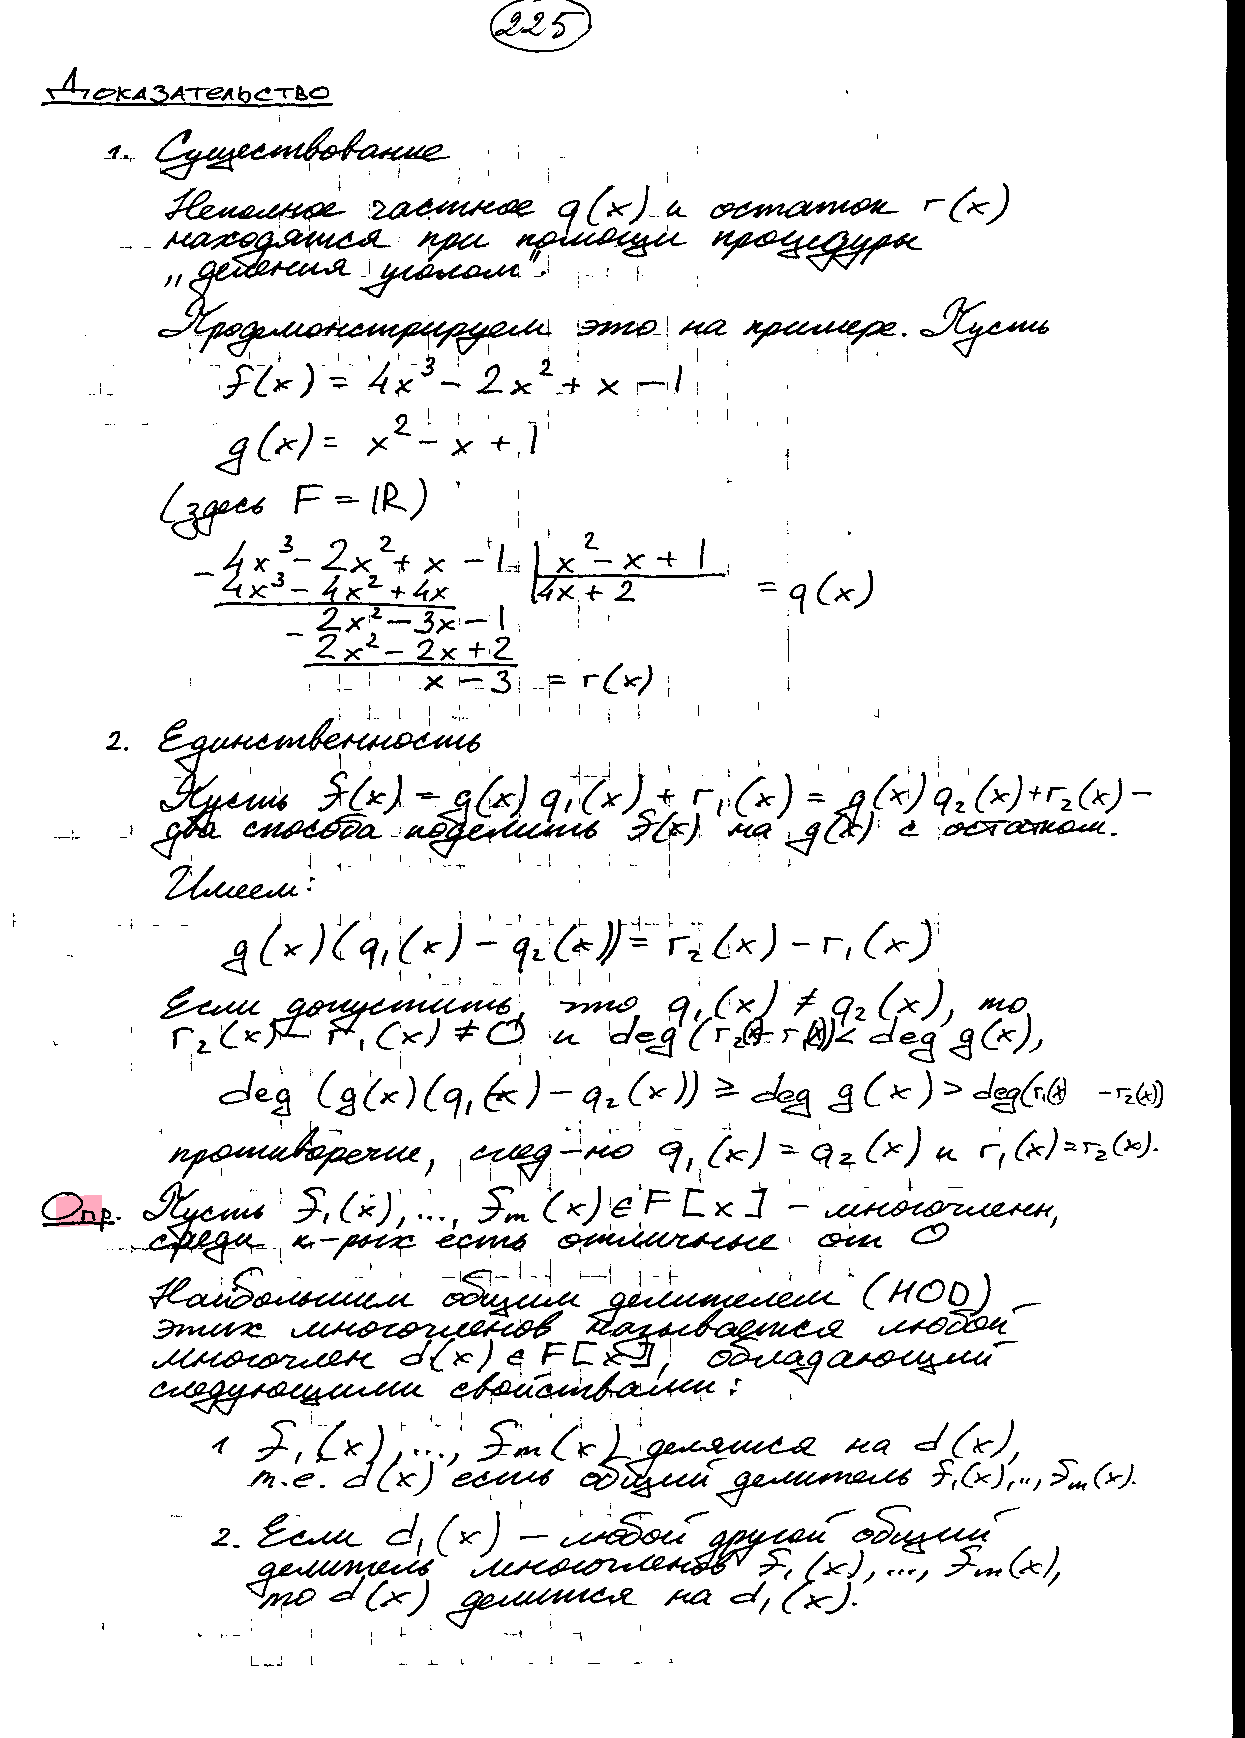
\includepdf[pages=-]{pdf/8_1.pdf}

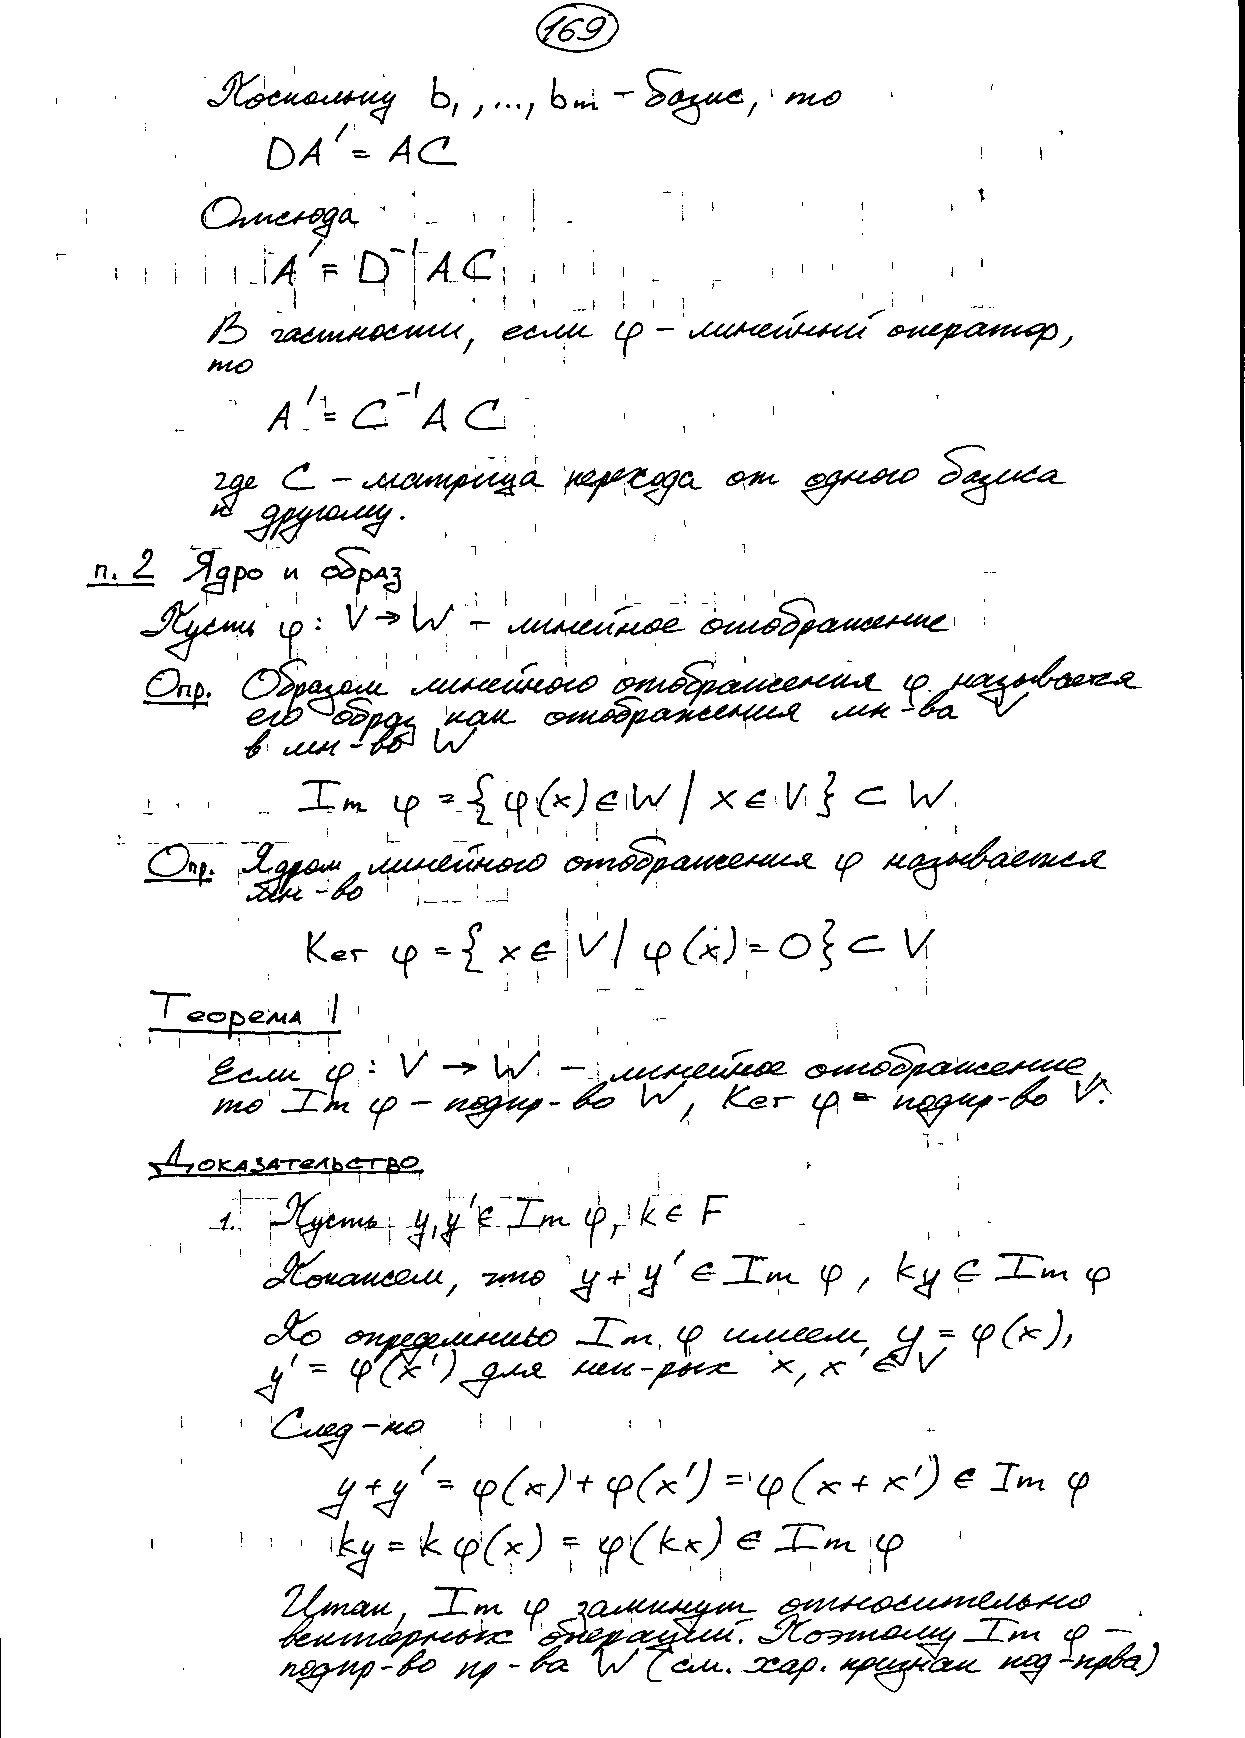
\includepdf[pages=-]{pdf/8_2.pdf}

\subsection{9. Линейная зависимость векторов. Базис и ранг конечной системы векторов.}
\label{sec:orgd671623}
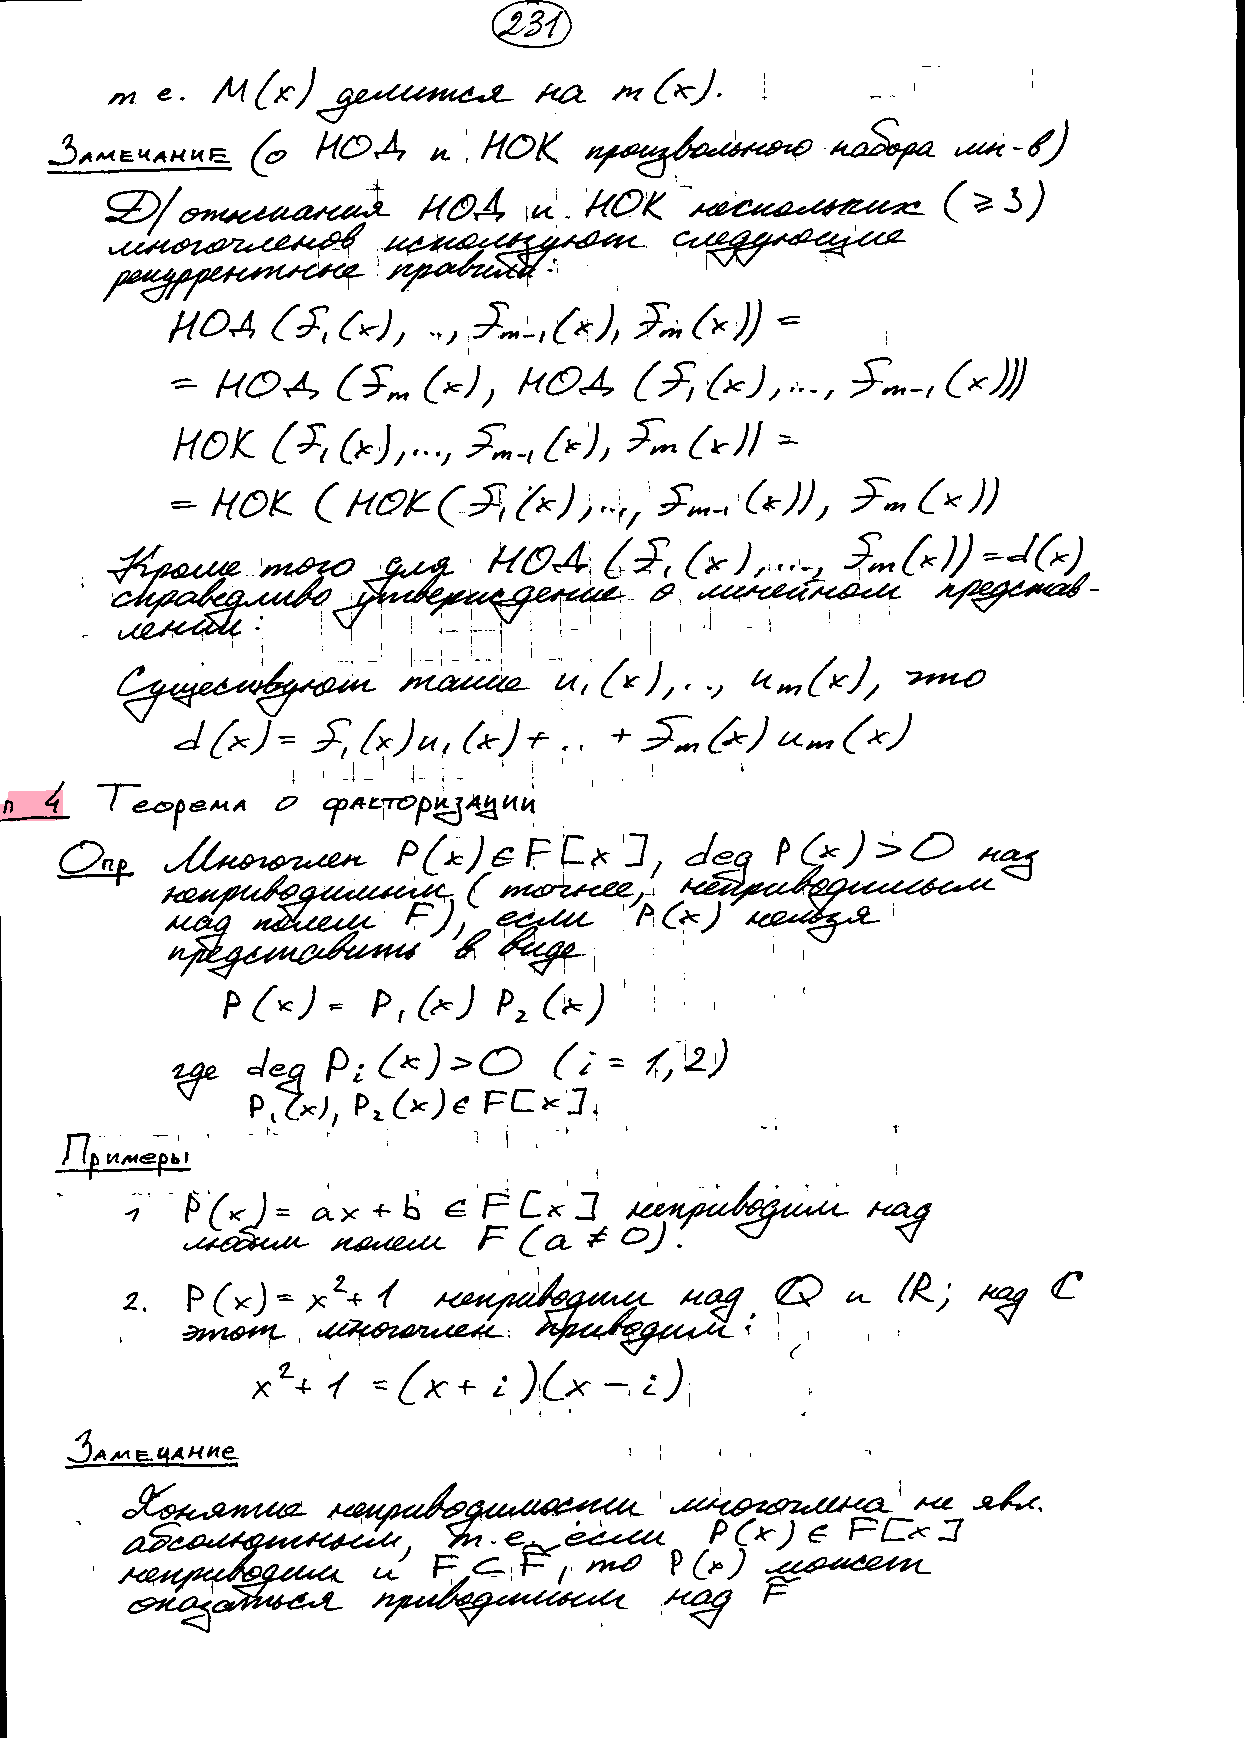
\includepdf[pages=-]{pdf/9_1.pdf}

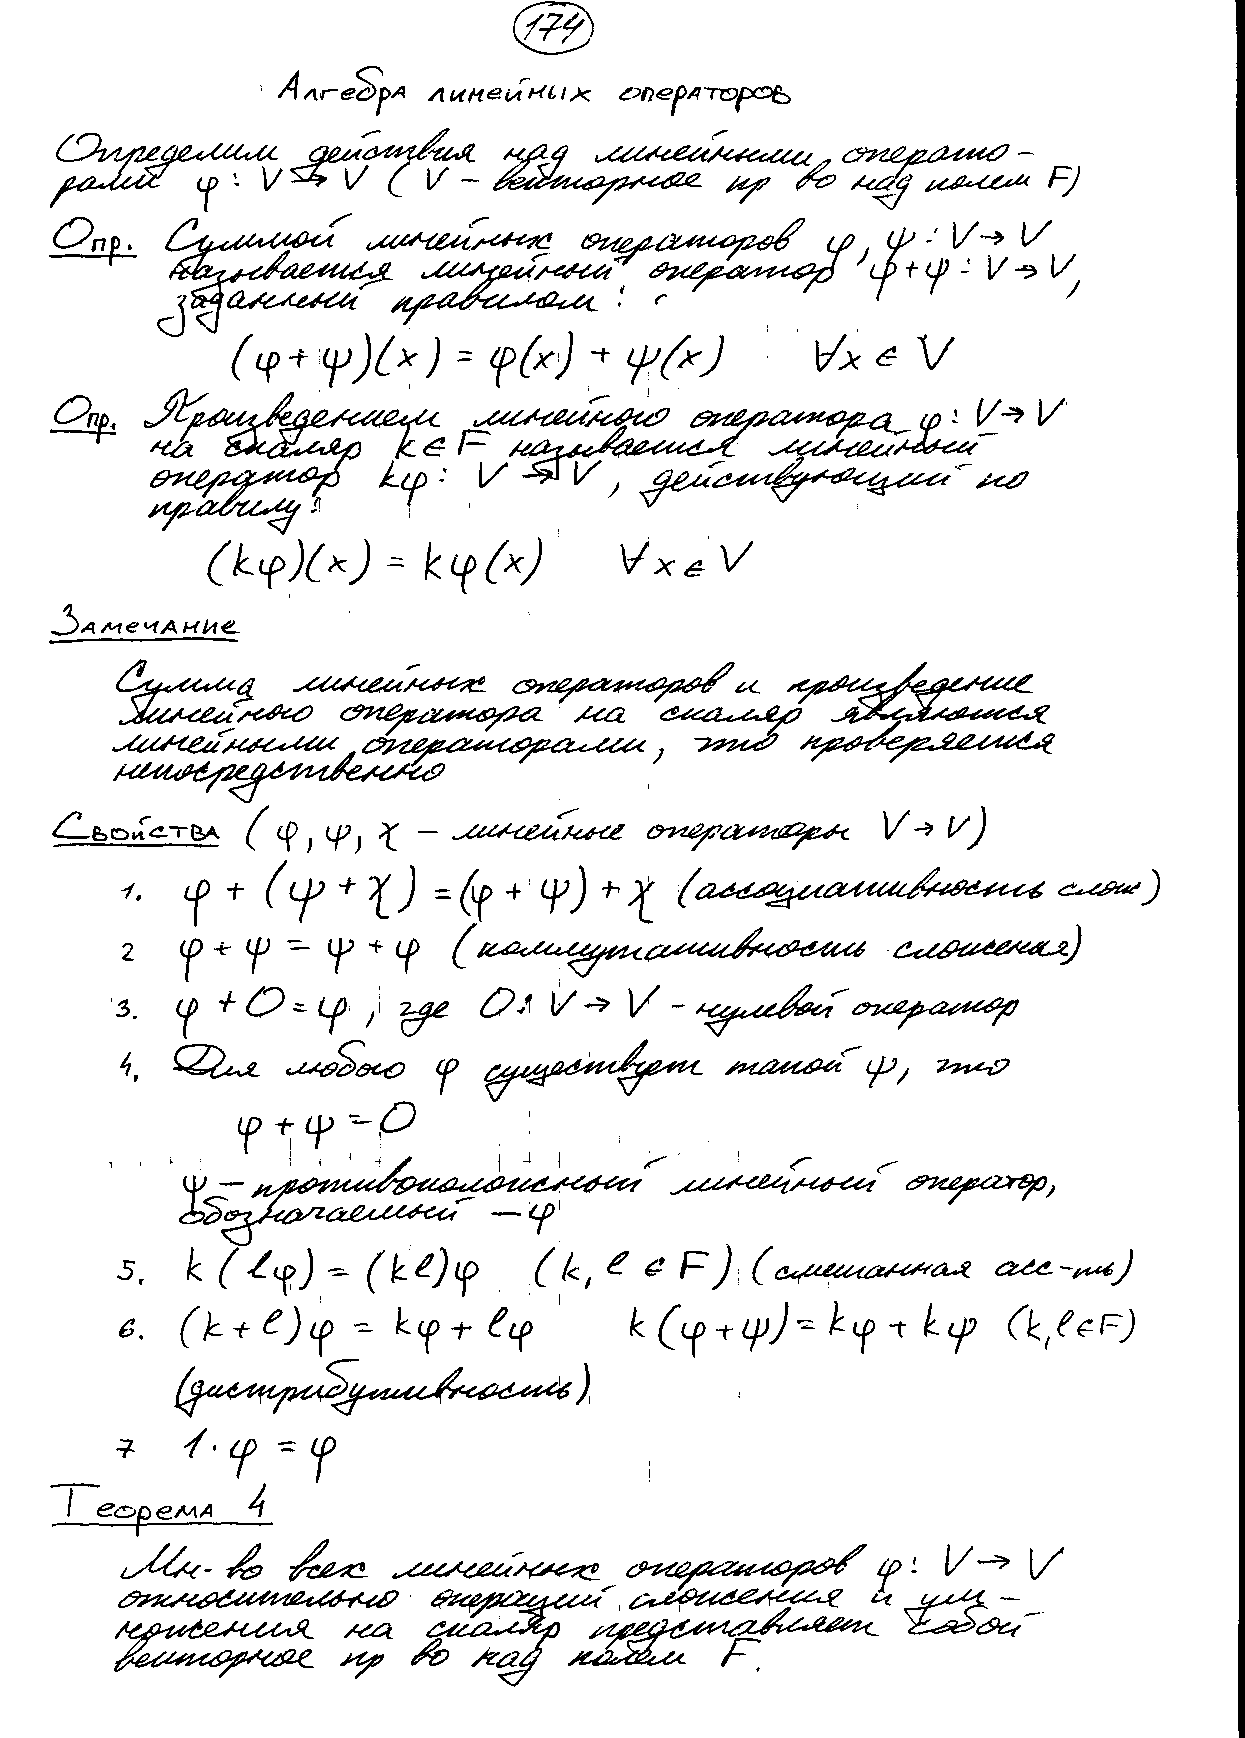
\includepdf[pages=-]{pdf/9_2.pdf}

\subsection{10. Базис векторного пространства. Конечномерные векторные пространства.}
\label{sec:orgea1d1e7}
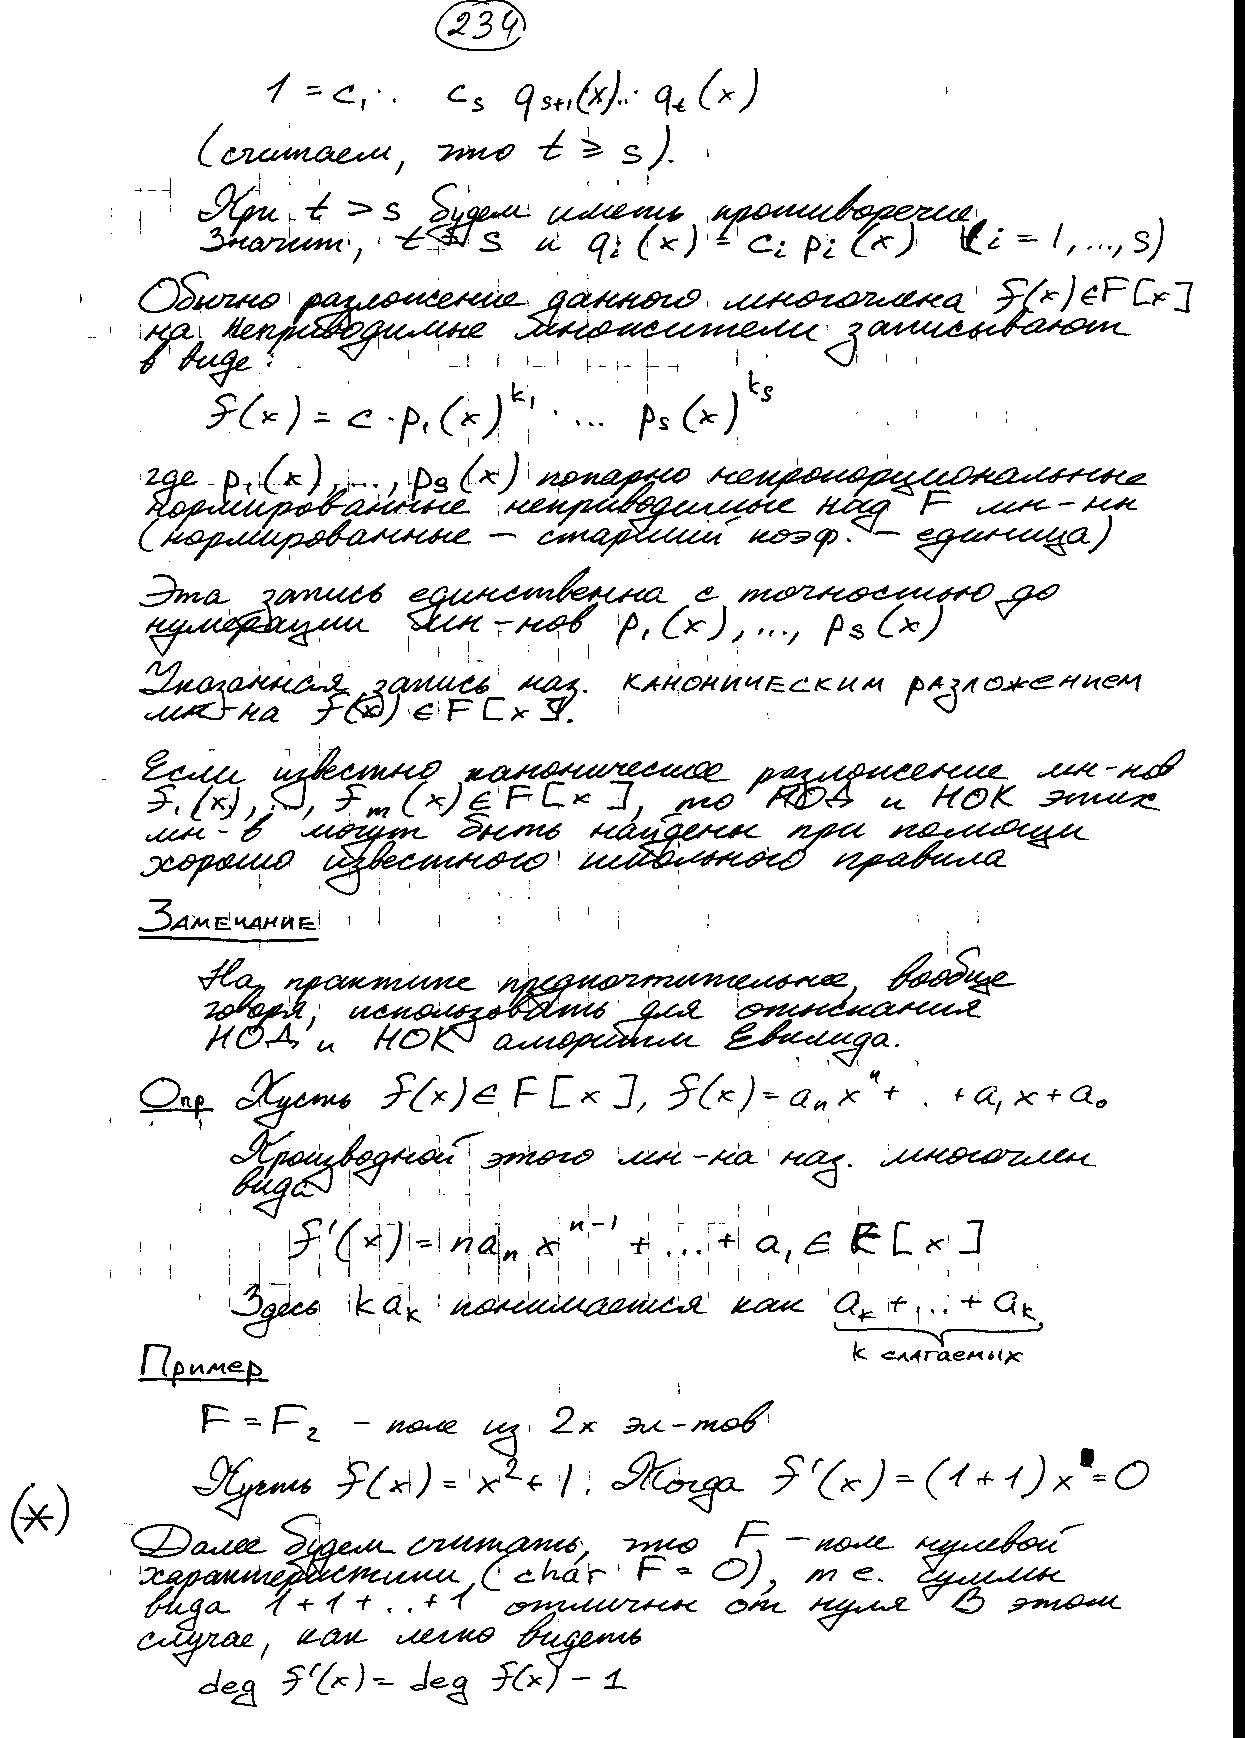
\includepdf[pages=-]{pdf/10_1.pdf}

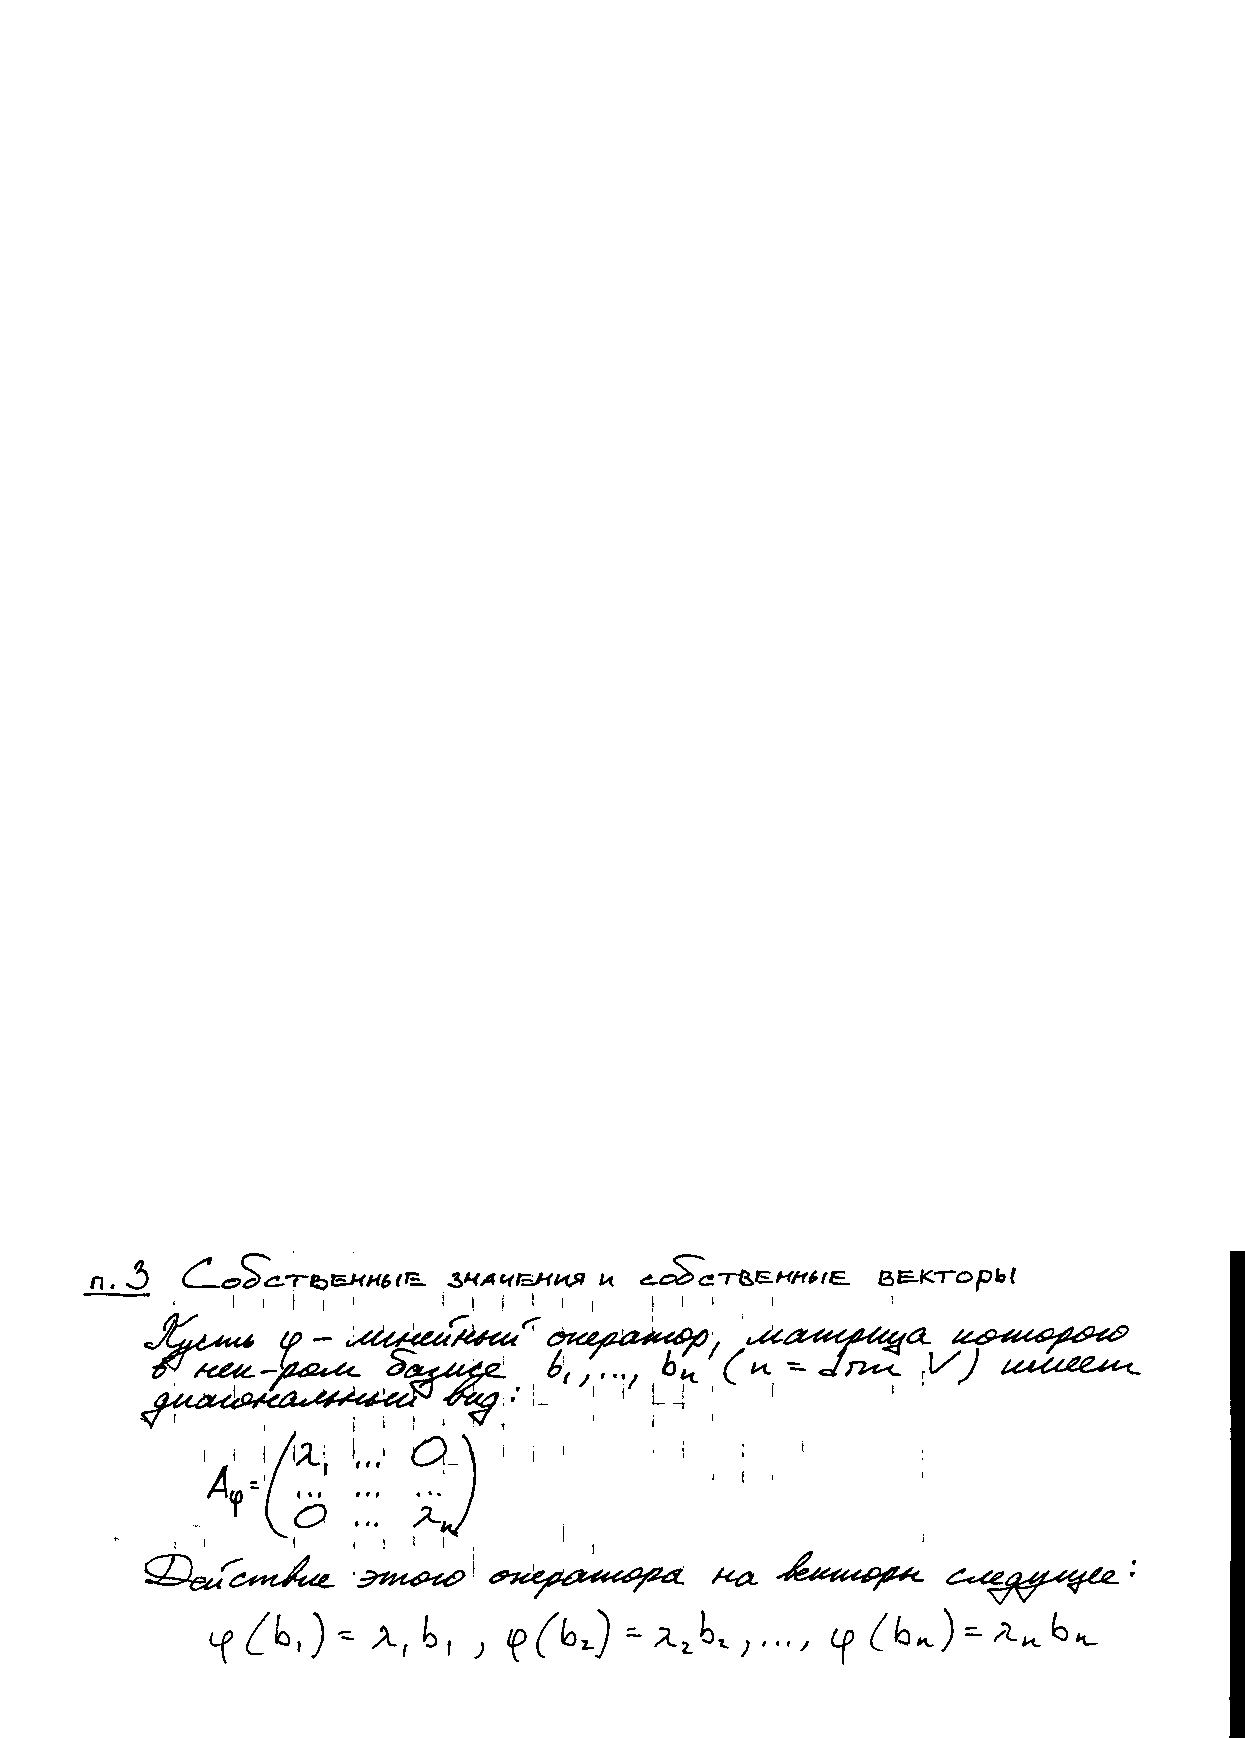
\includepdf[pages=-]{pdf/10_2.pdf}

\subsection{11. Координаты вектора в базисе. Матрица перехода от одного базиса к другому. Связь между координатами вектора в разных базисах.}
\label{sec:org6c6694c}
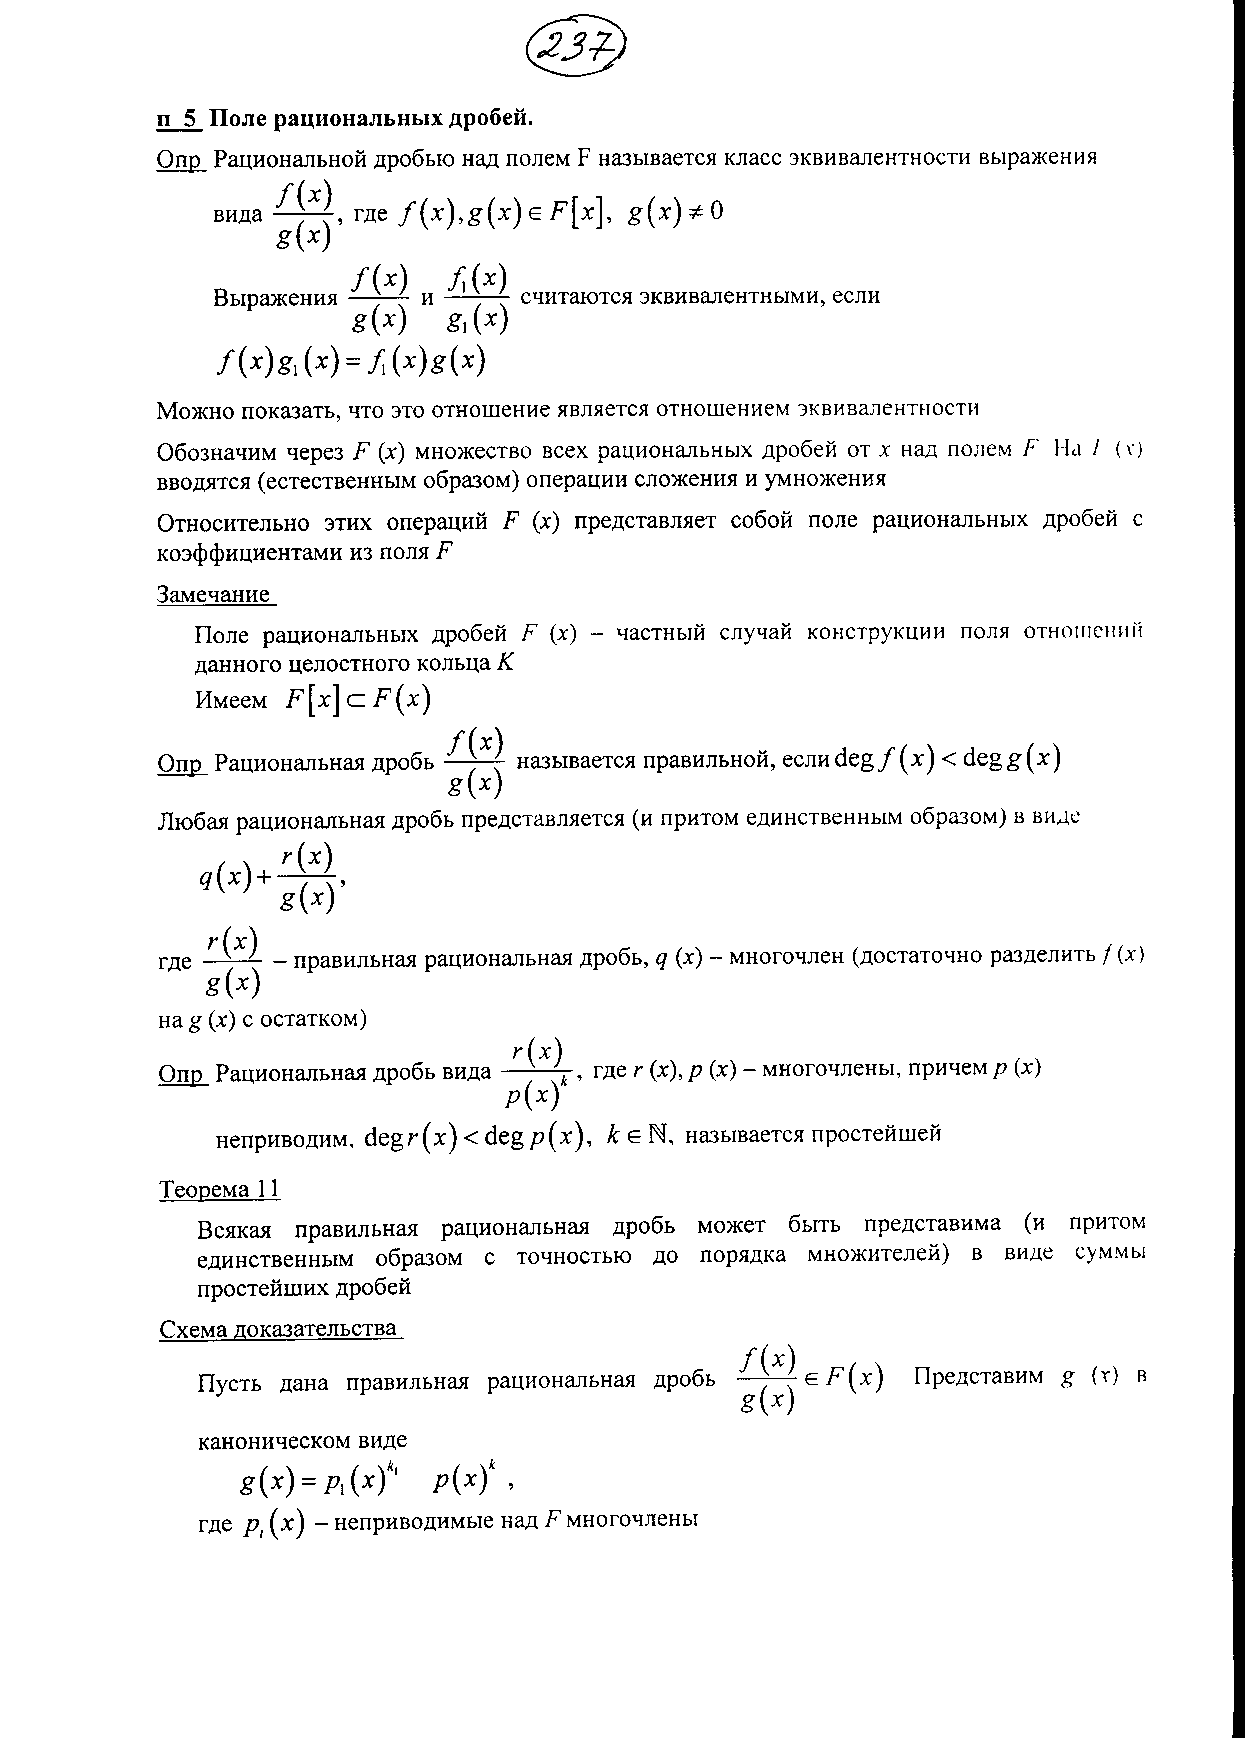
\includepdf[pages=-]{pdf/11_1.pdf}

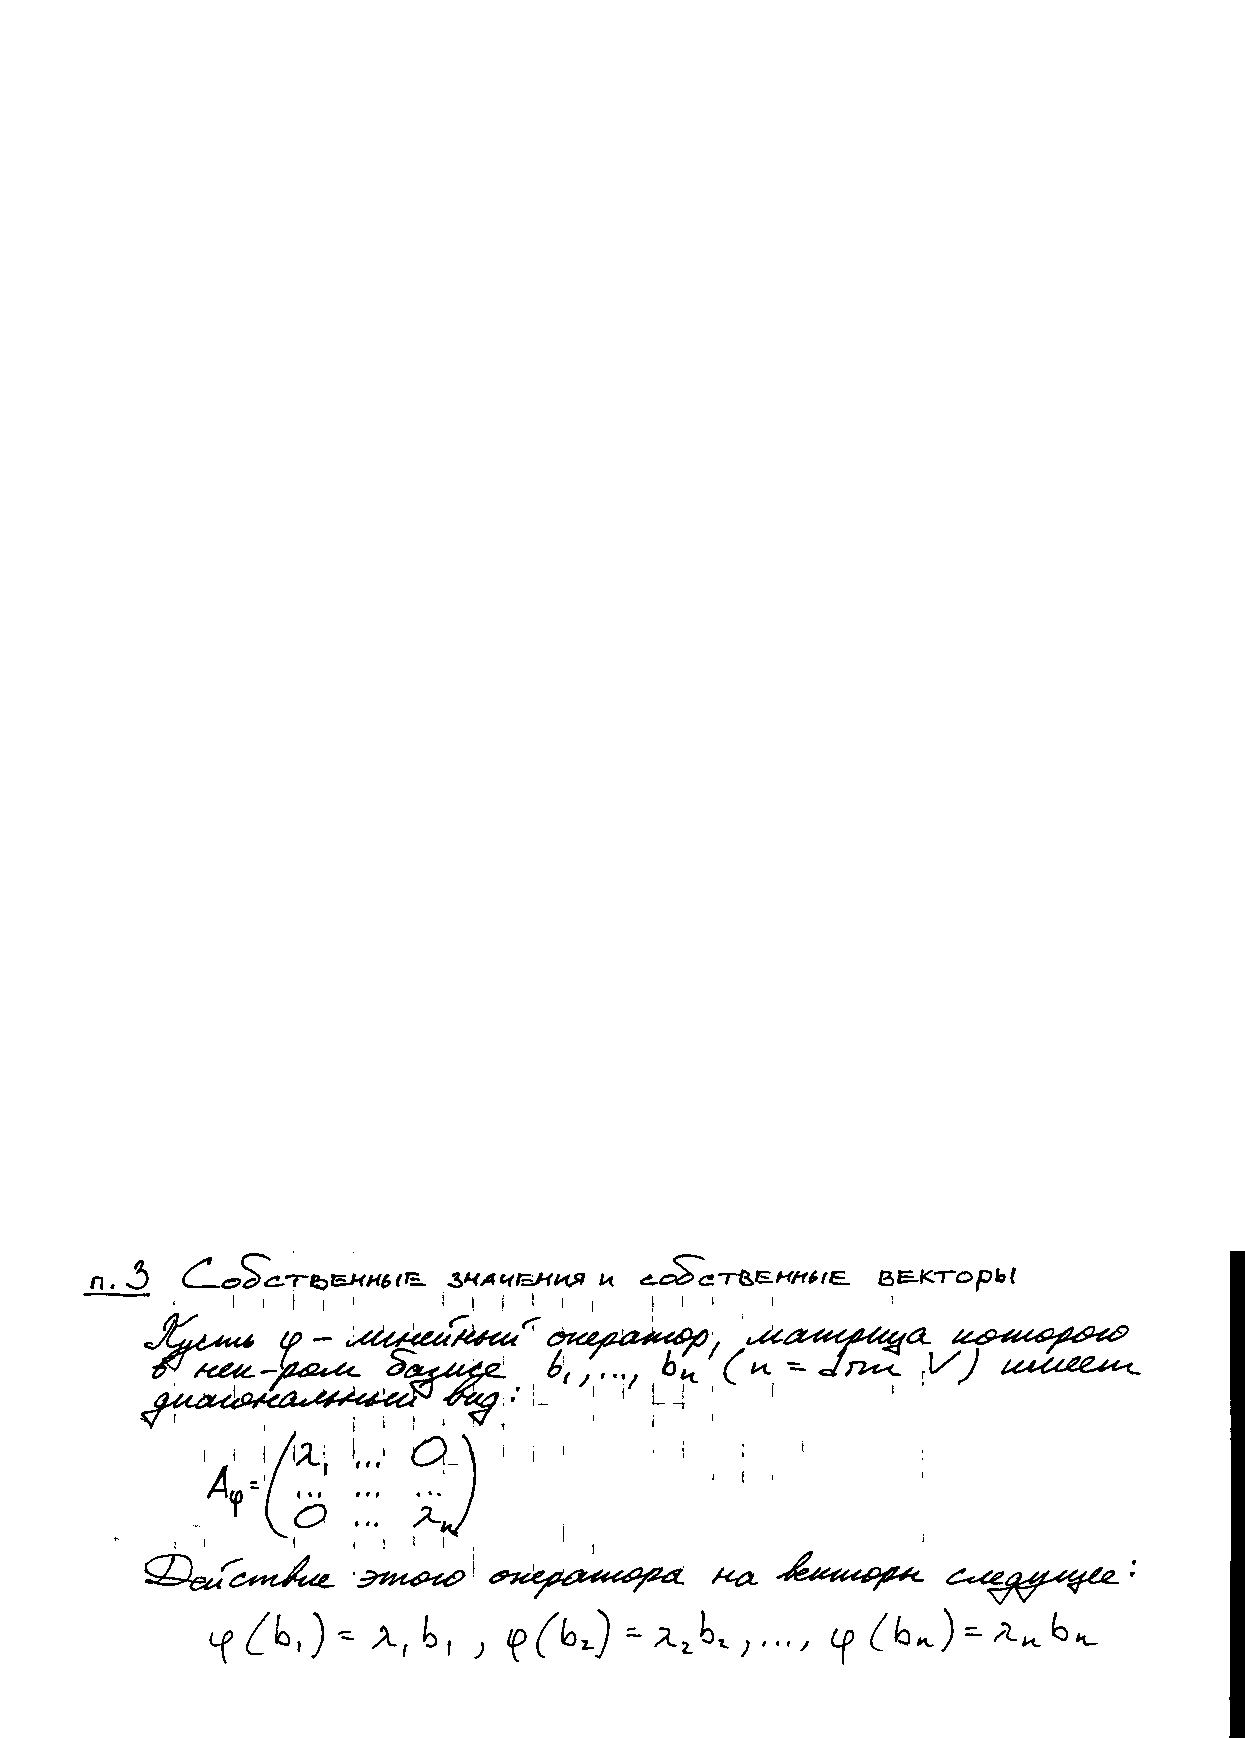
\includepdf[pages=-]{pdf/11_2.pdf}

\subsection{12. Линейная оболочка системы векторов. Суммы подпространств.}
\label{sec:org5550f82}
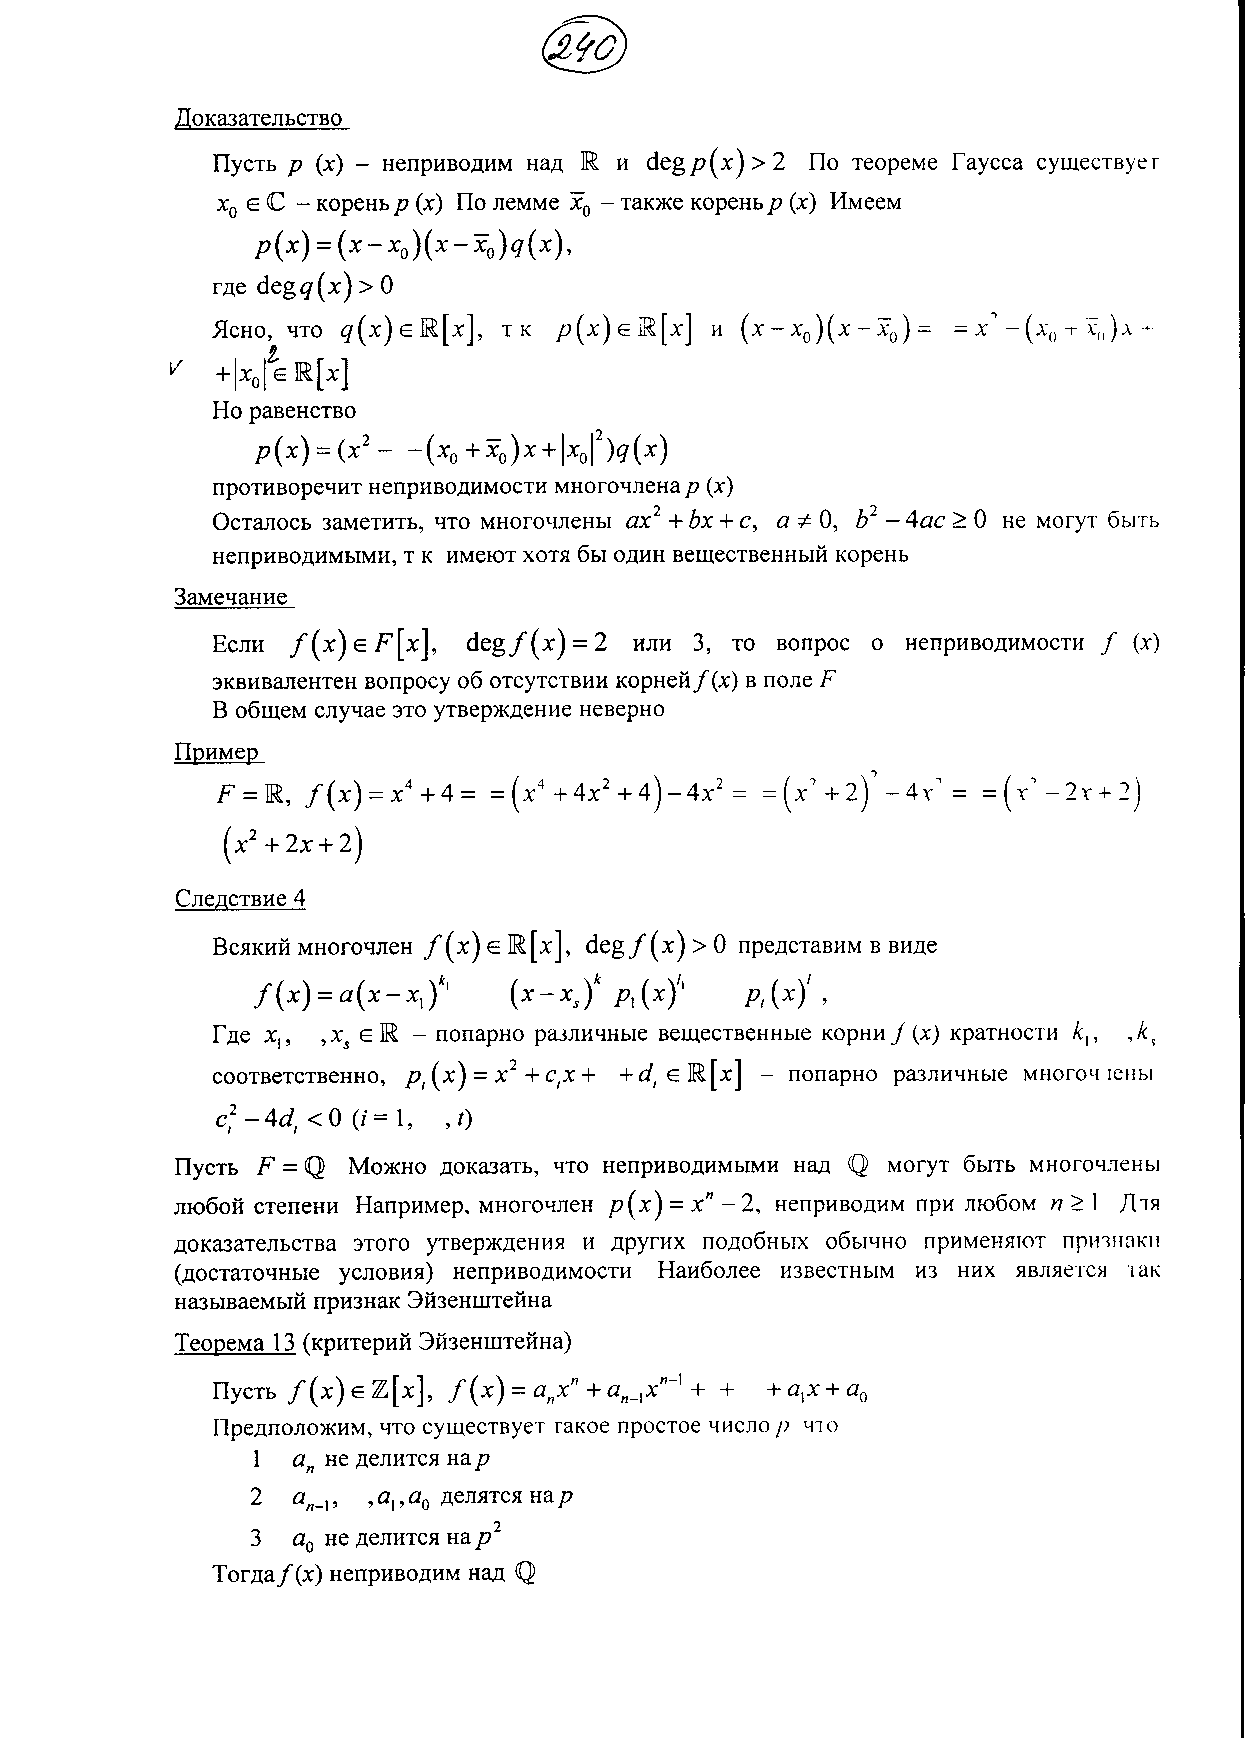
\includepdf[pages=-]{pdf/12_1.pdf}

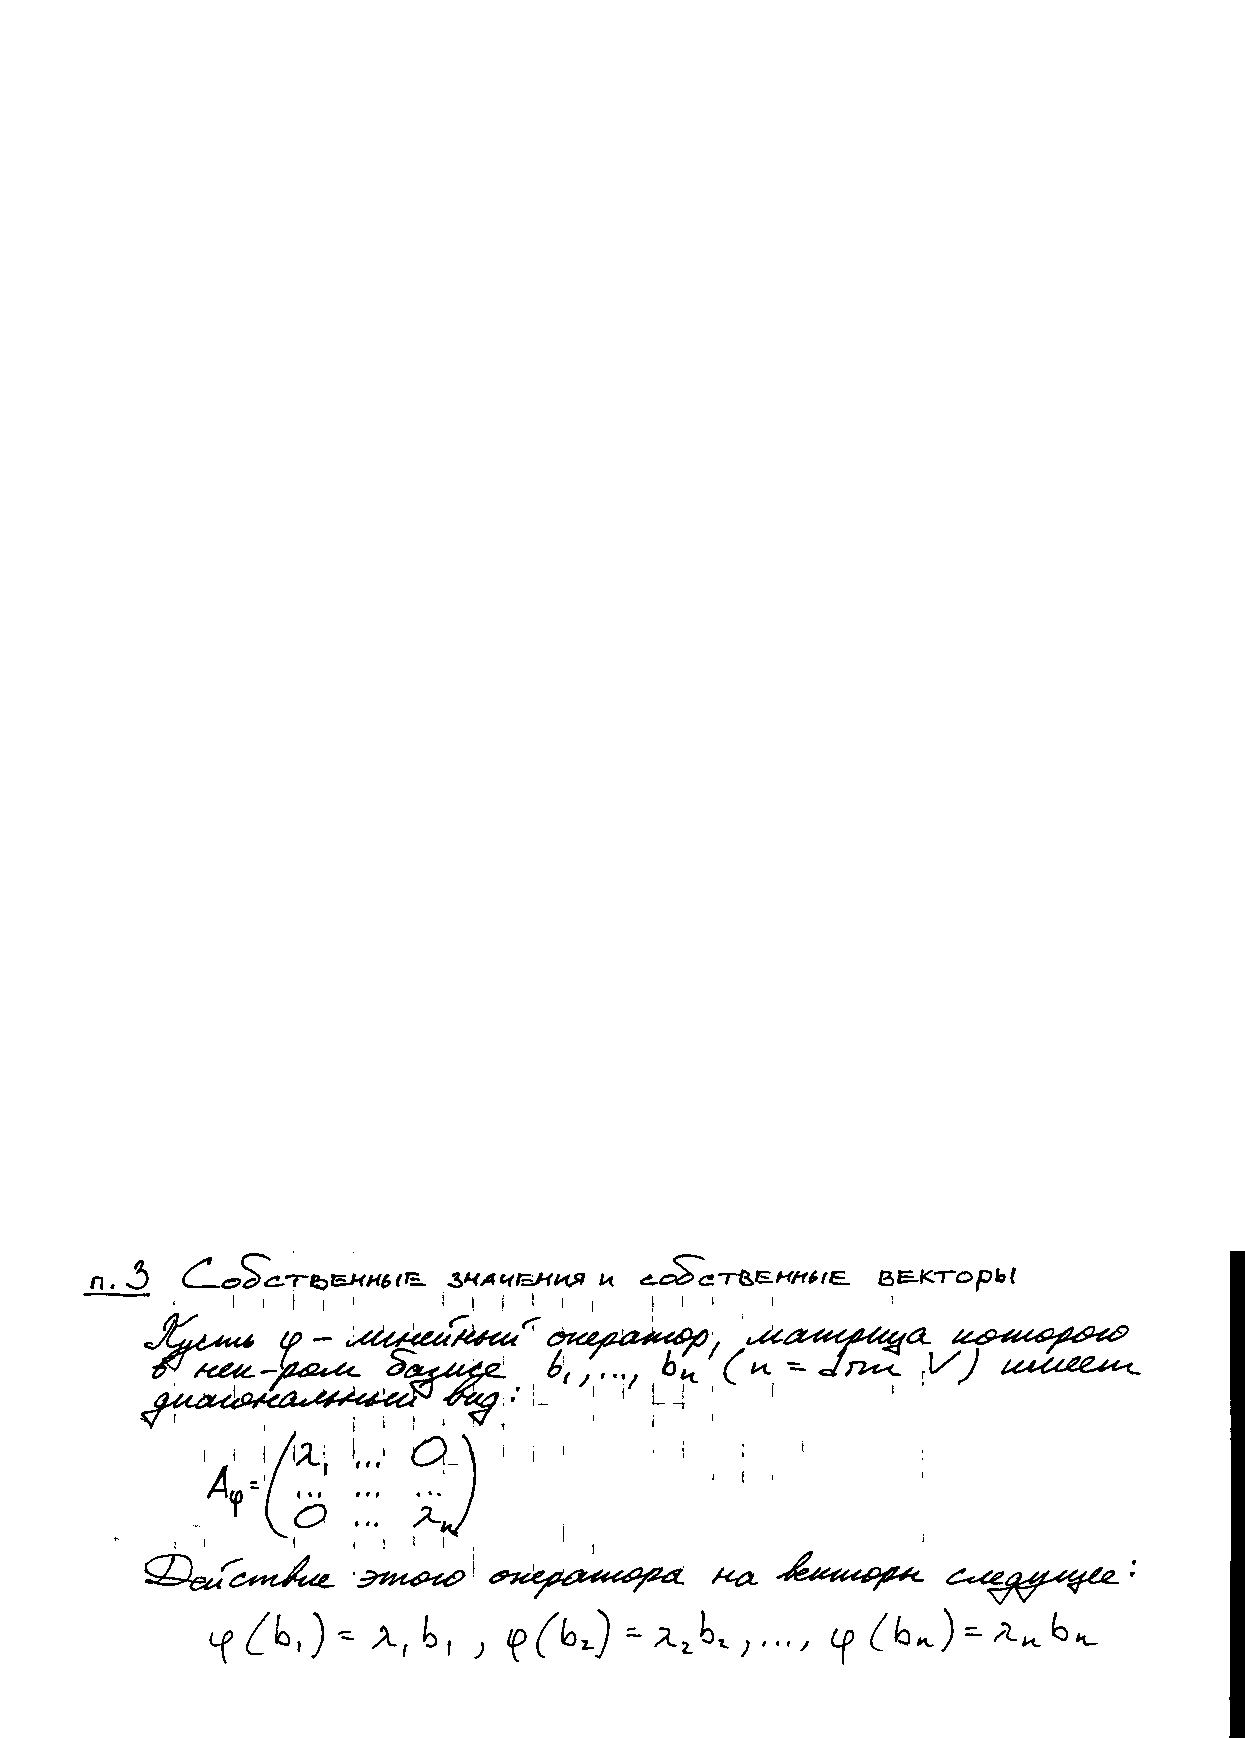
\includepdf[pages=-]{pdf/12_2.pdf}

\subsection{13. Скалярное произведение в вещественном векторном пространстве. Ортогональные векторы. Линейная независимость ортогональной системы ненулевых векторов.}
\label{sec:orgc610b73}
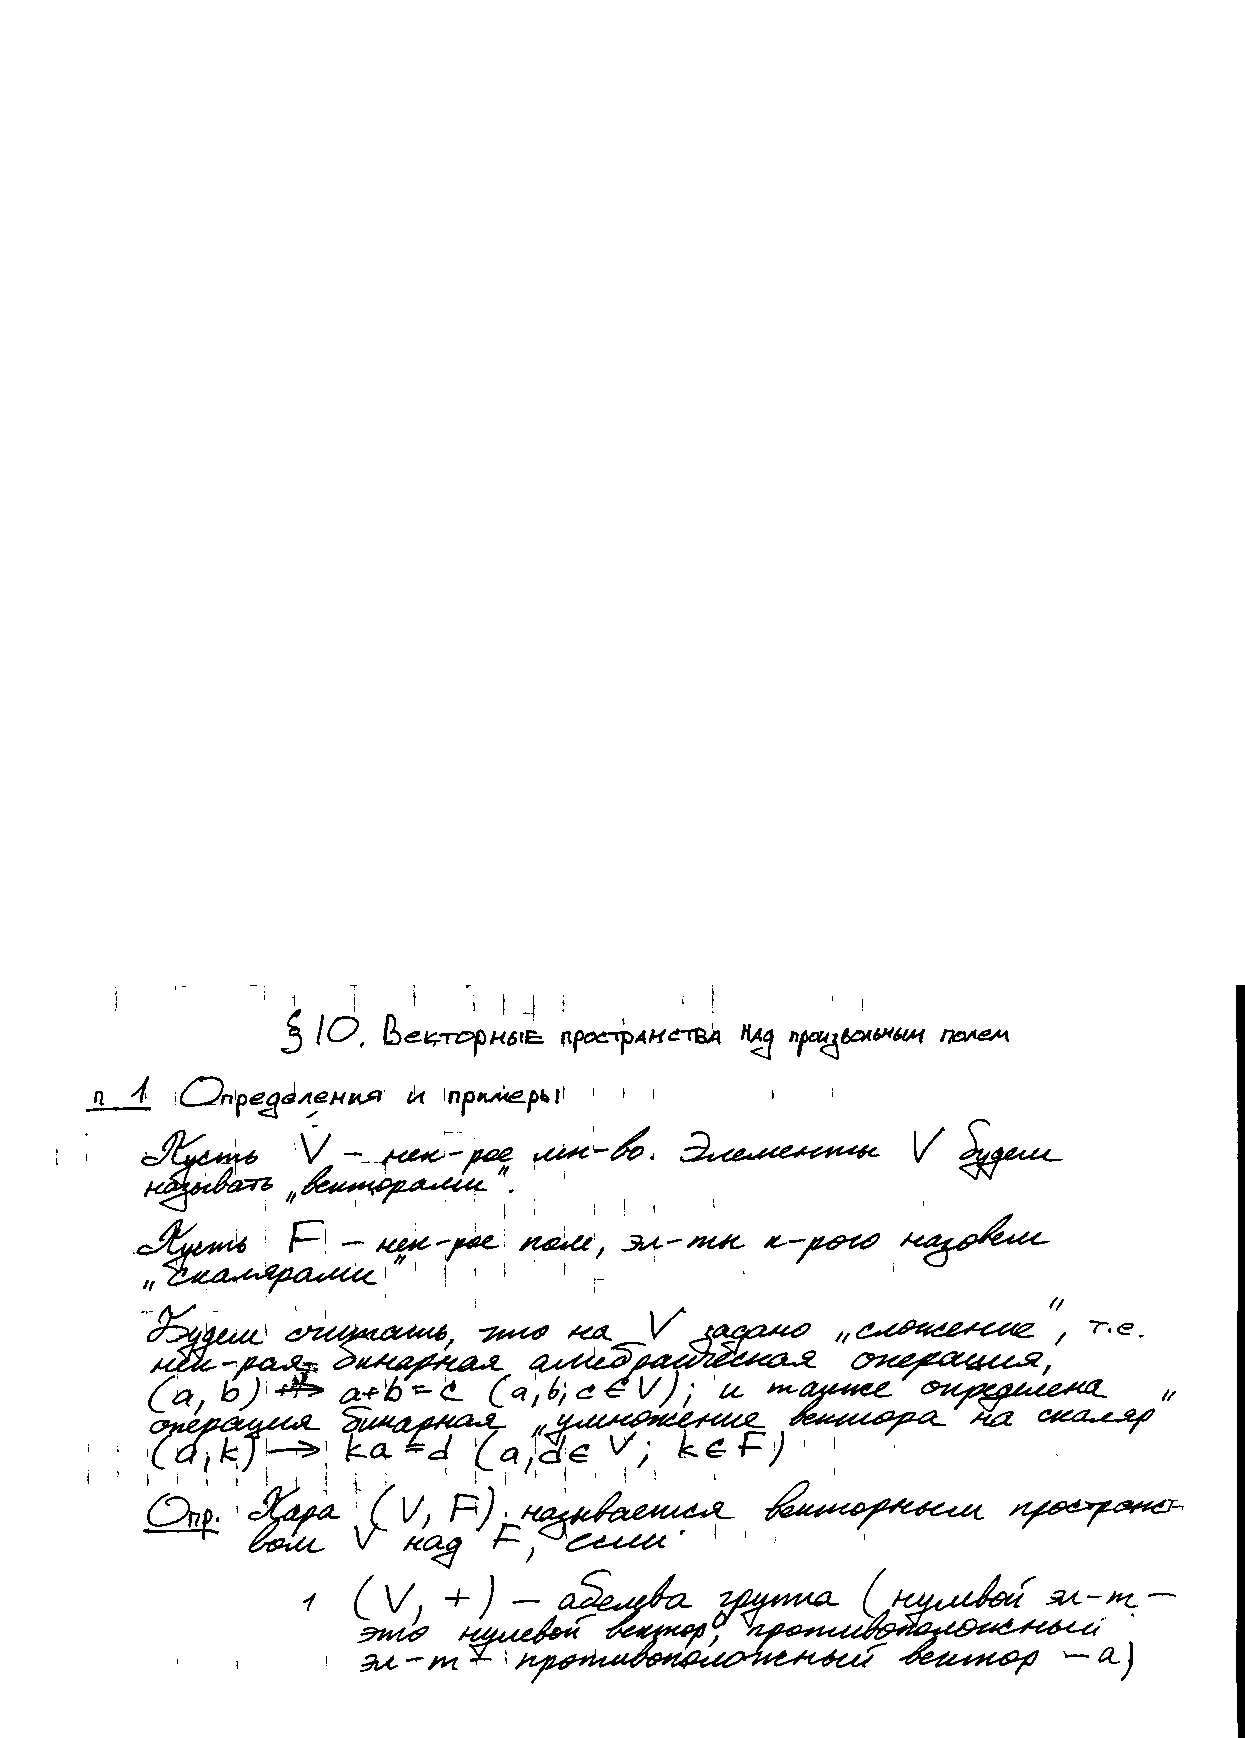
\includepdf[pages=-]{pdf/13_1.pdf}

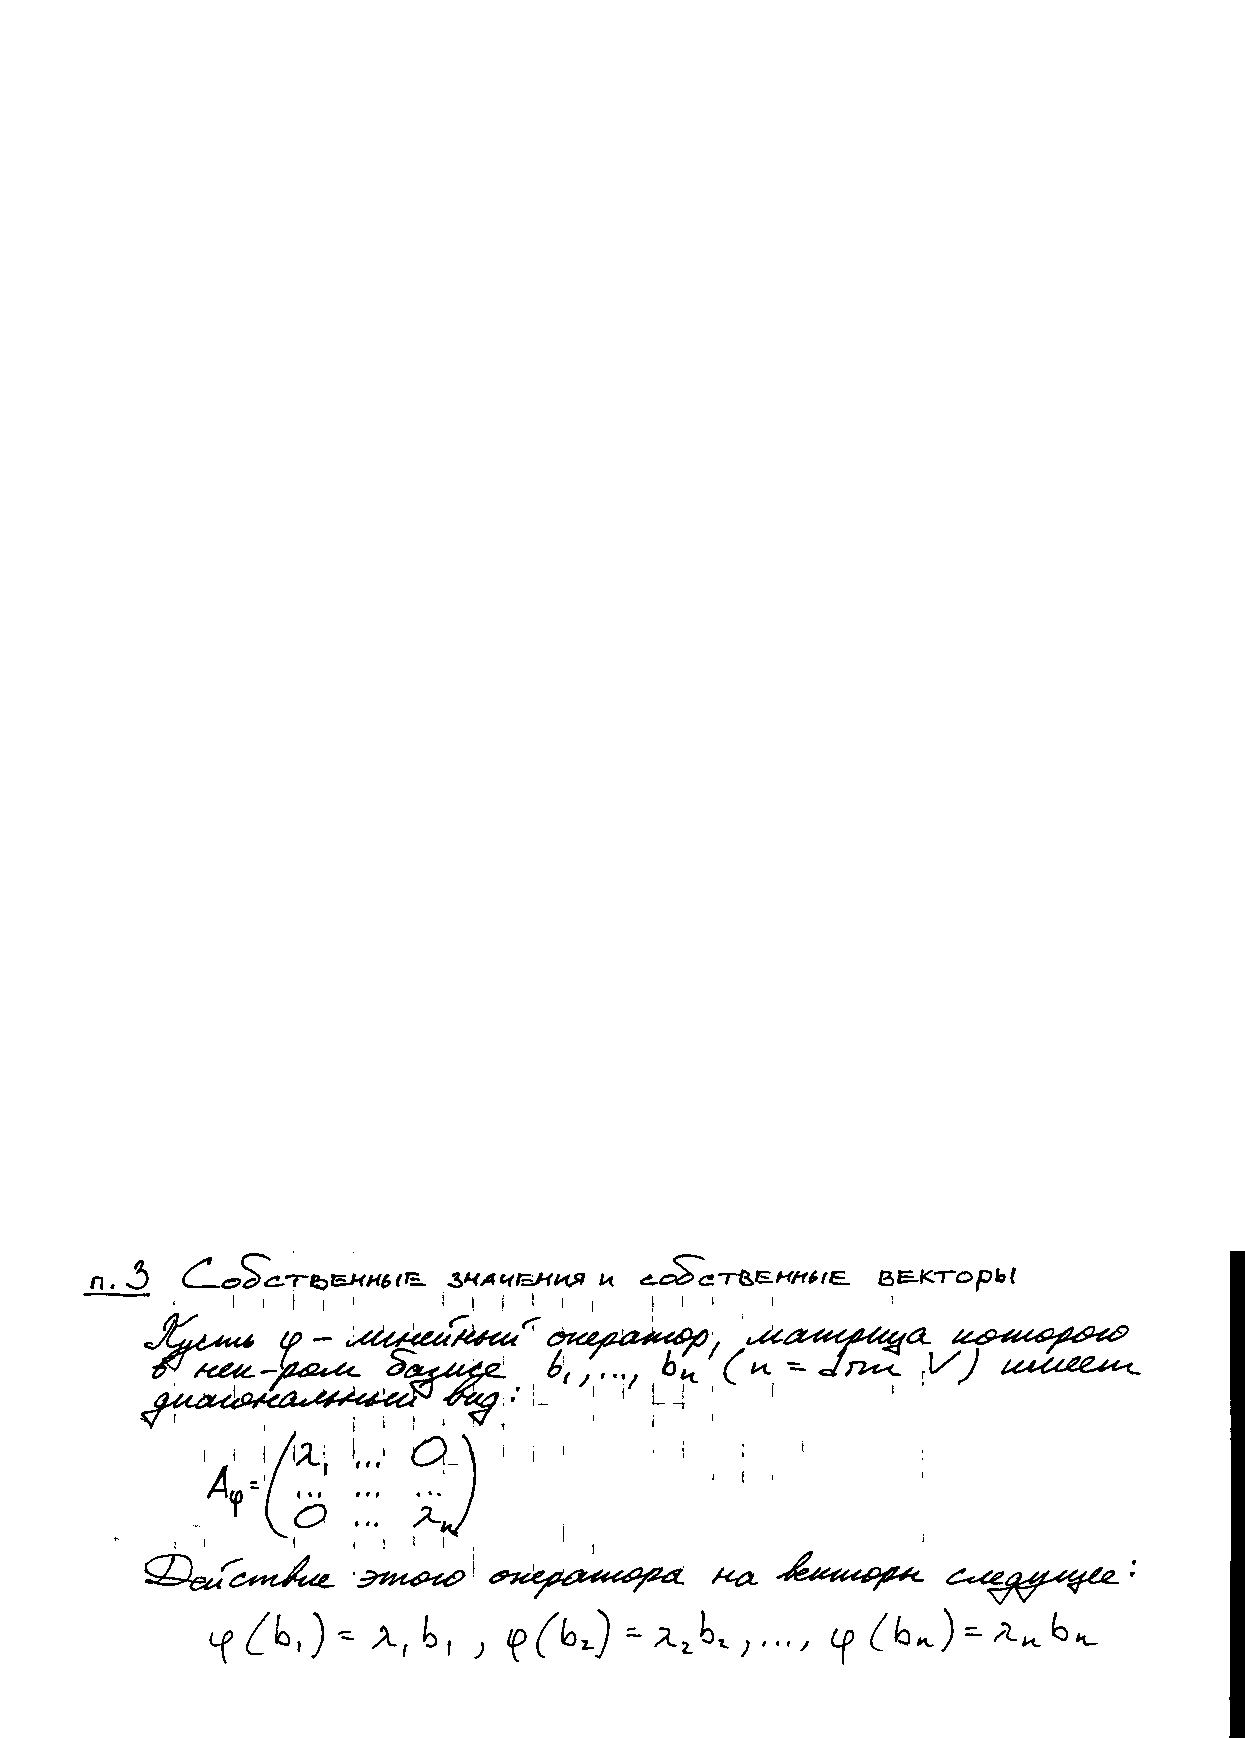
\includepdf[pages=-]{pdf/13_2.pdf}

\subsection{14. Евклидово пространство. Матрица Грама скалярного произведения в базисе и её изменение при переходе к другому базису.}
\label{sec:org7c89ed1}
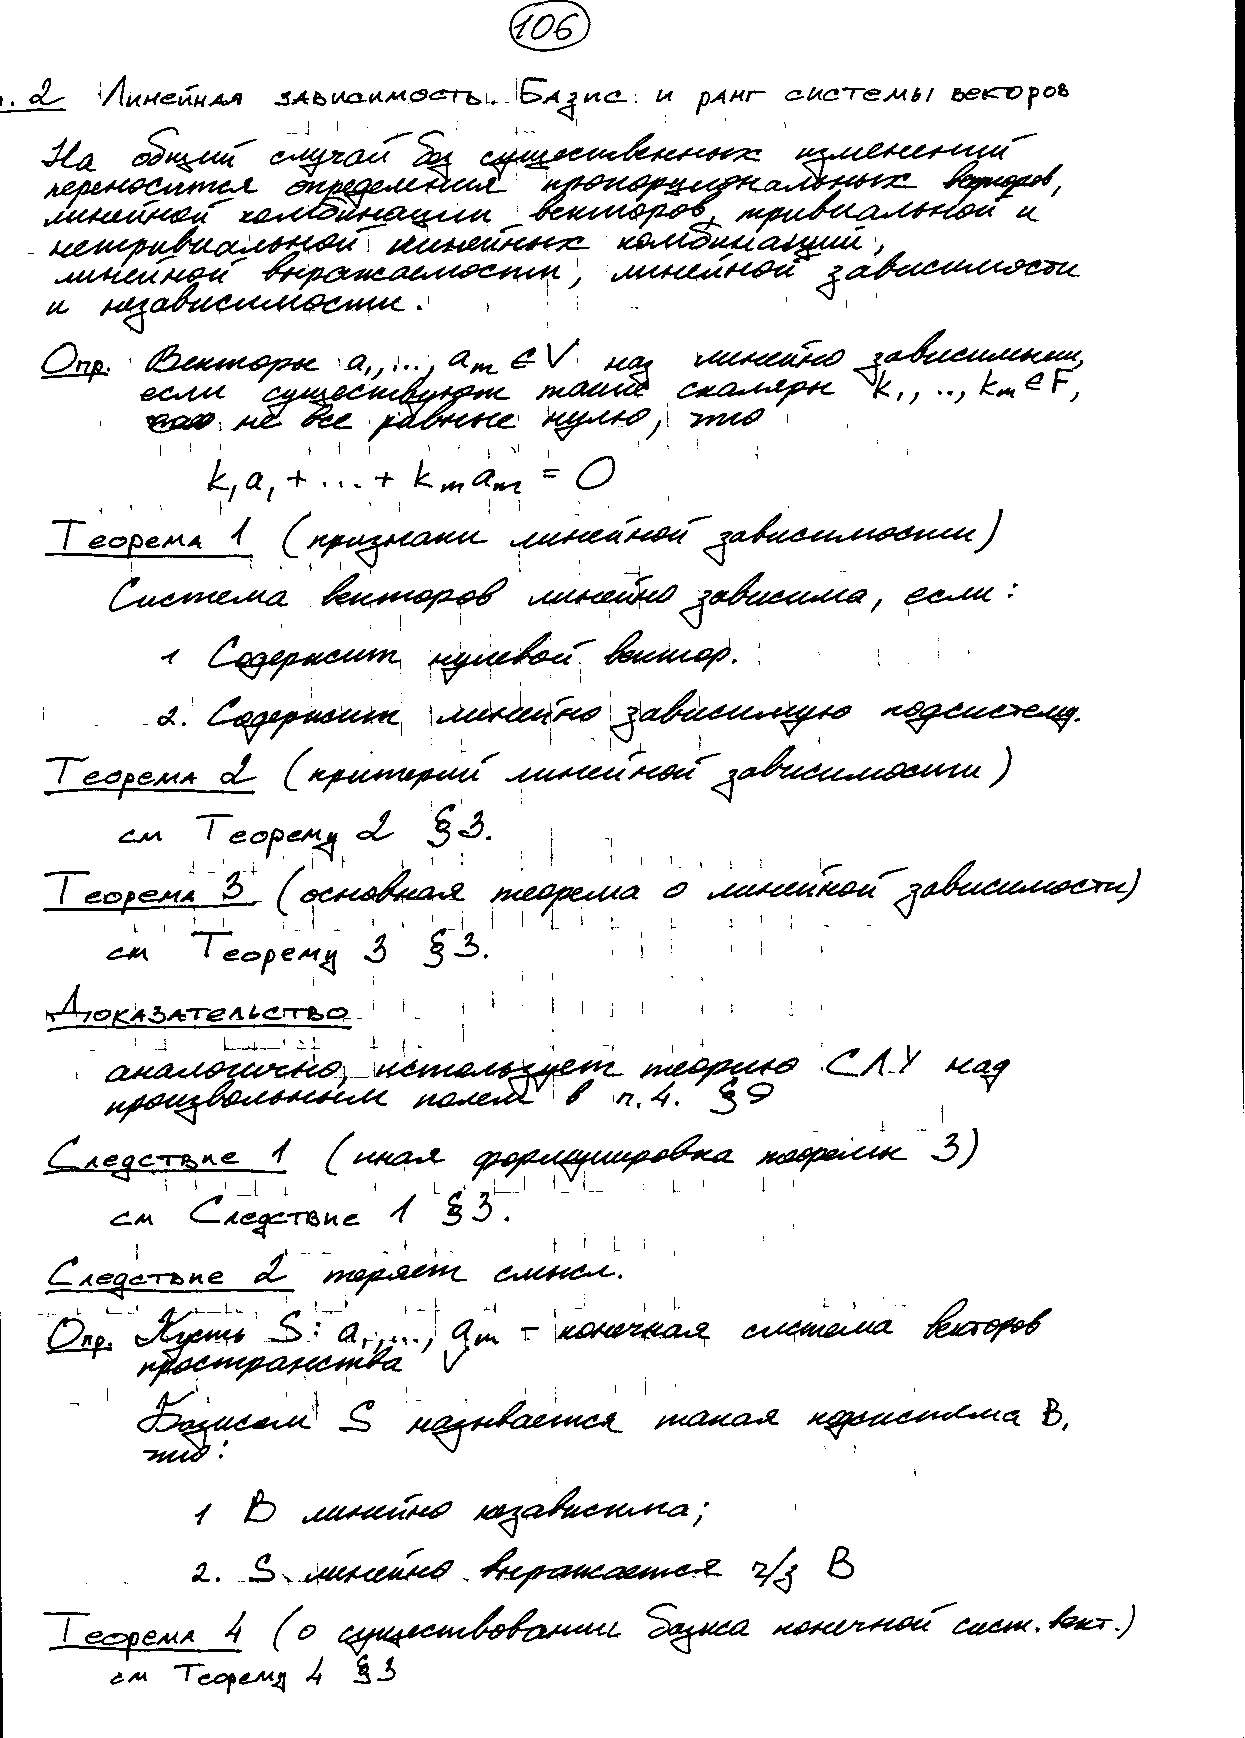
\includepdf[pages=-]{pdf/14_1.pdf}

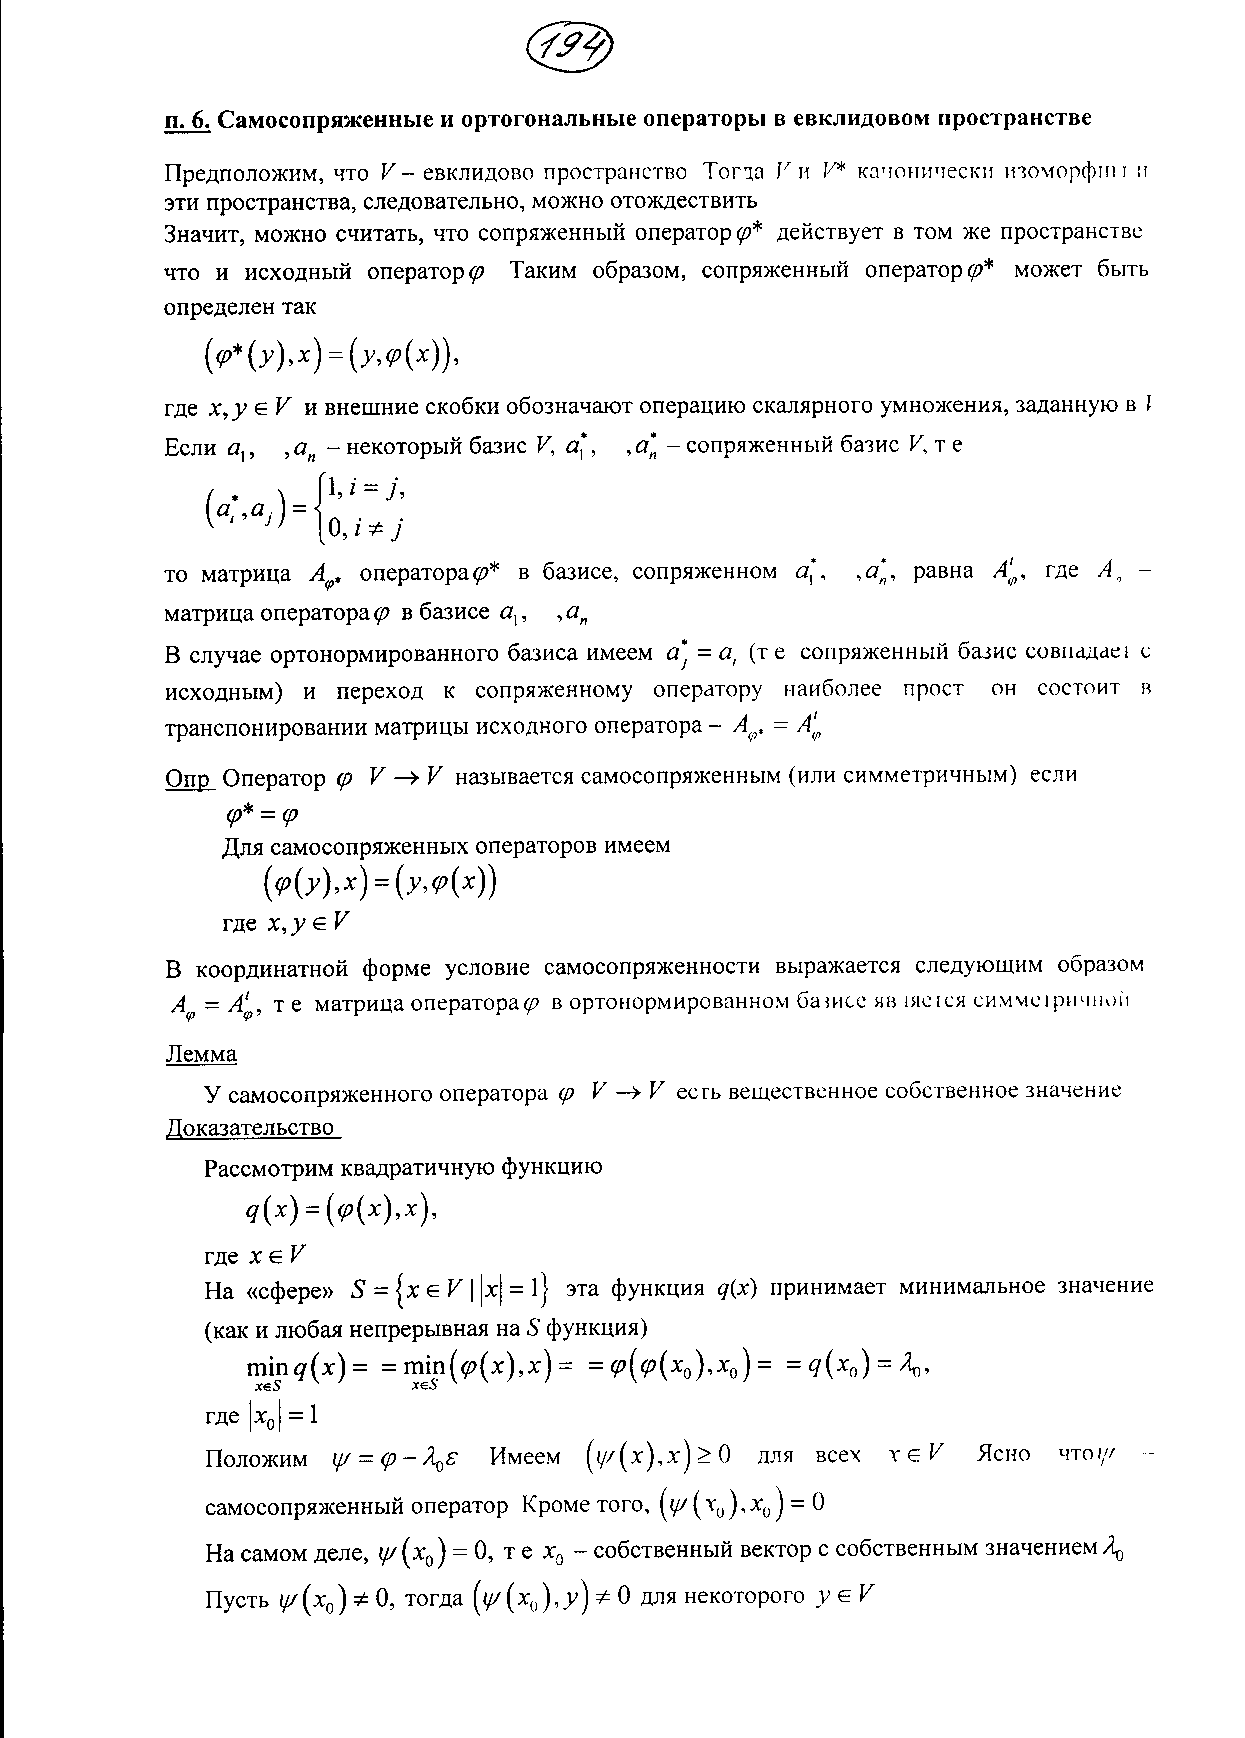
\includepdf[pages=-]{pdf/14_2.pdf}

\subsection{15. Ортогональные и ортонормированные базисы в евклидовом пространстве. Процесс ортогонализации Грамма—Шмидта.}
\label{sec:orgd0d61b9}
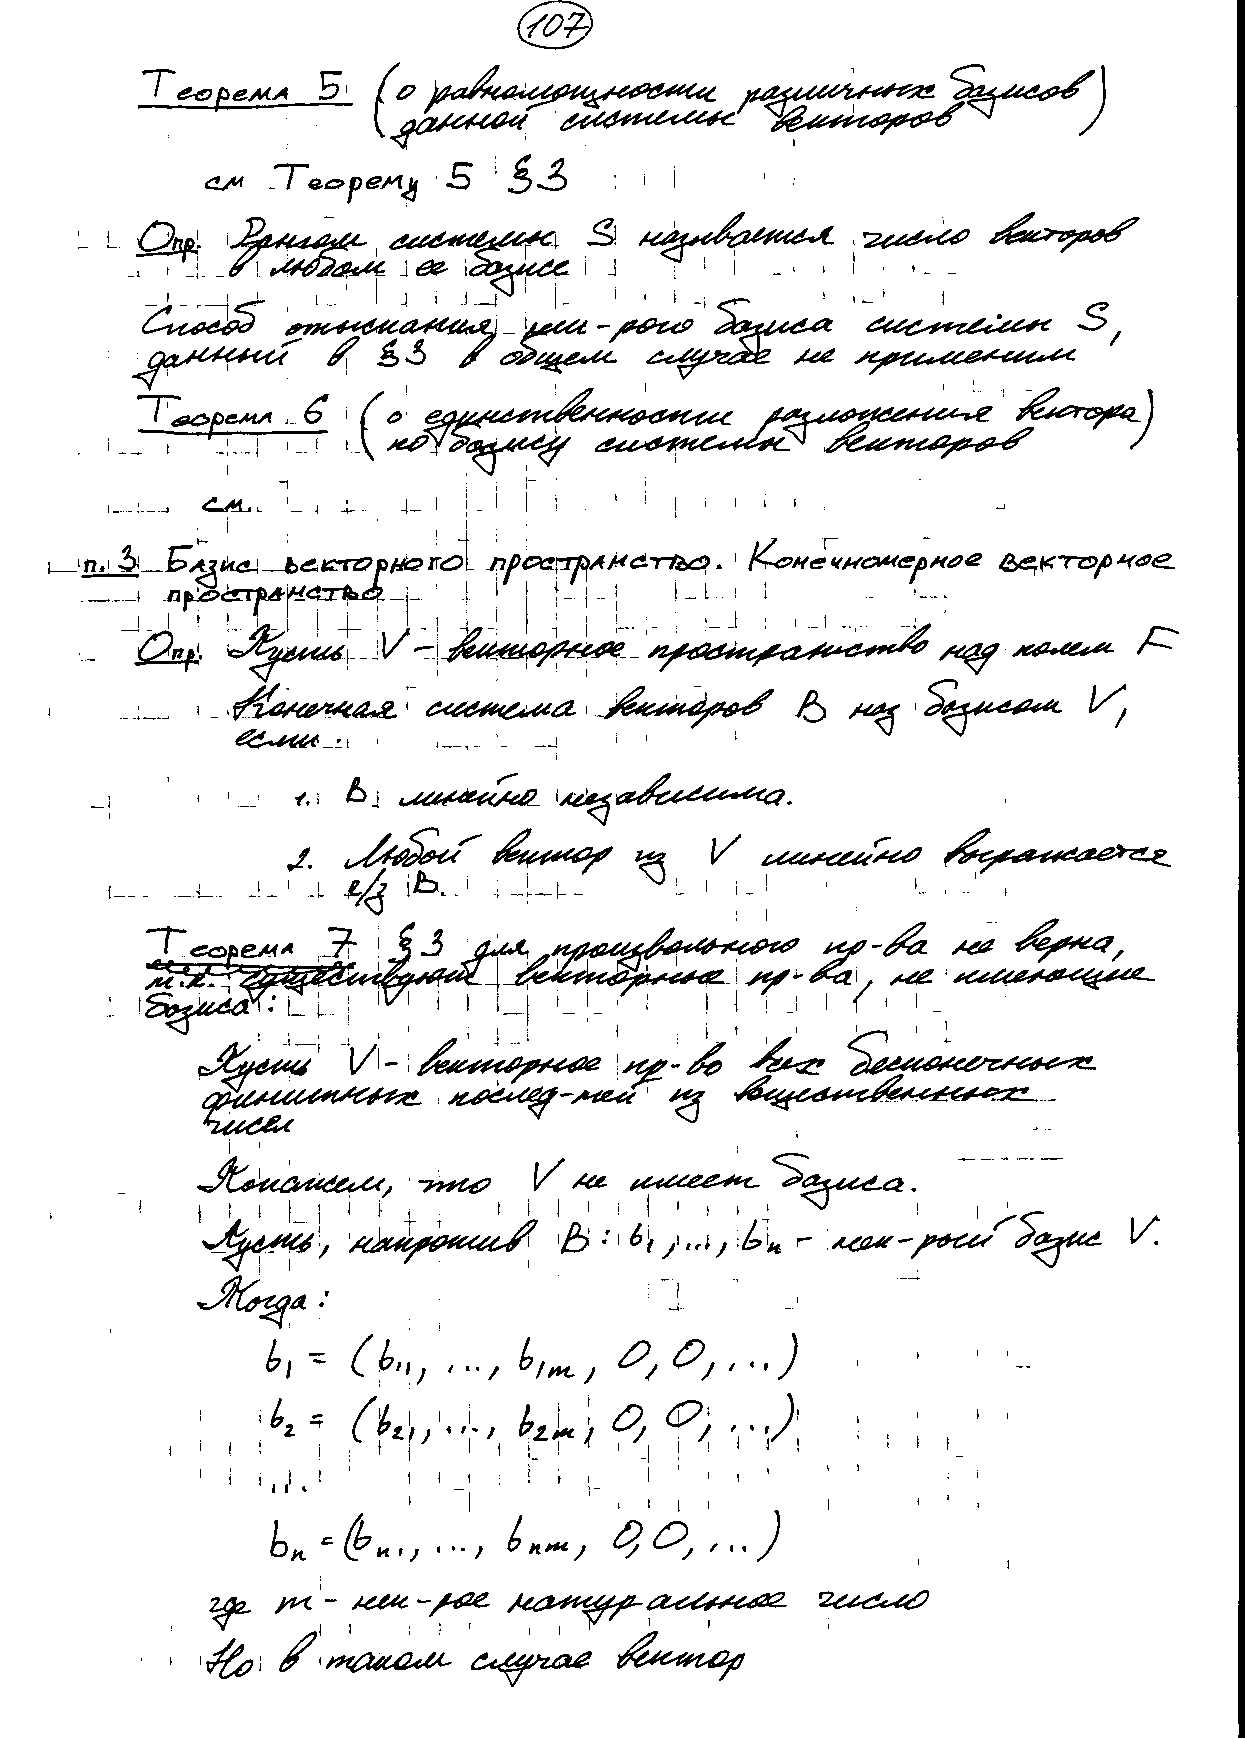
\includepdf[pages=-]{pdf/15_1.pdf}

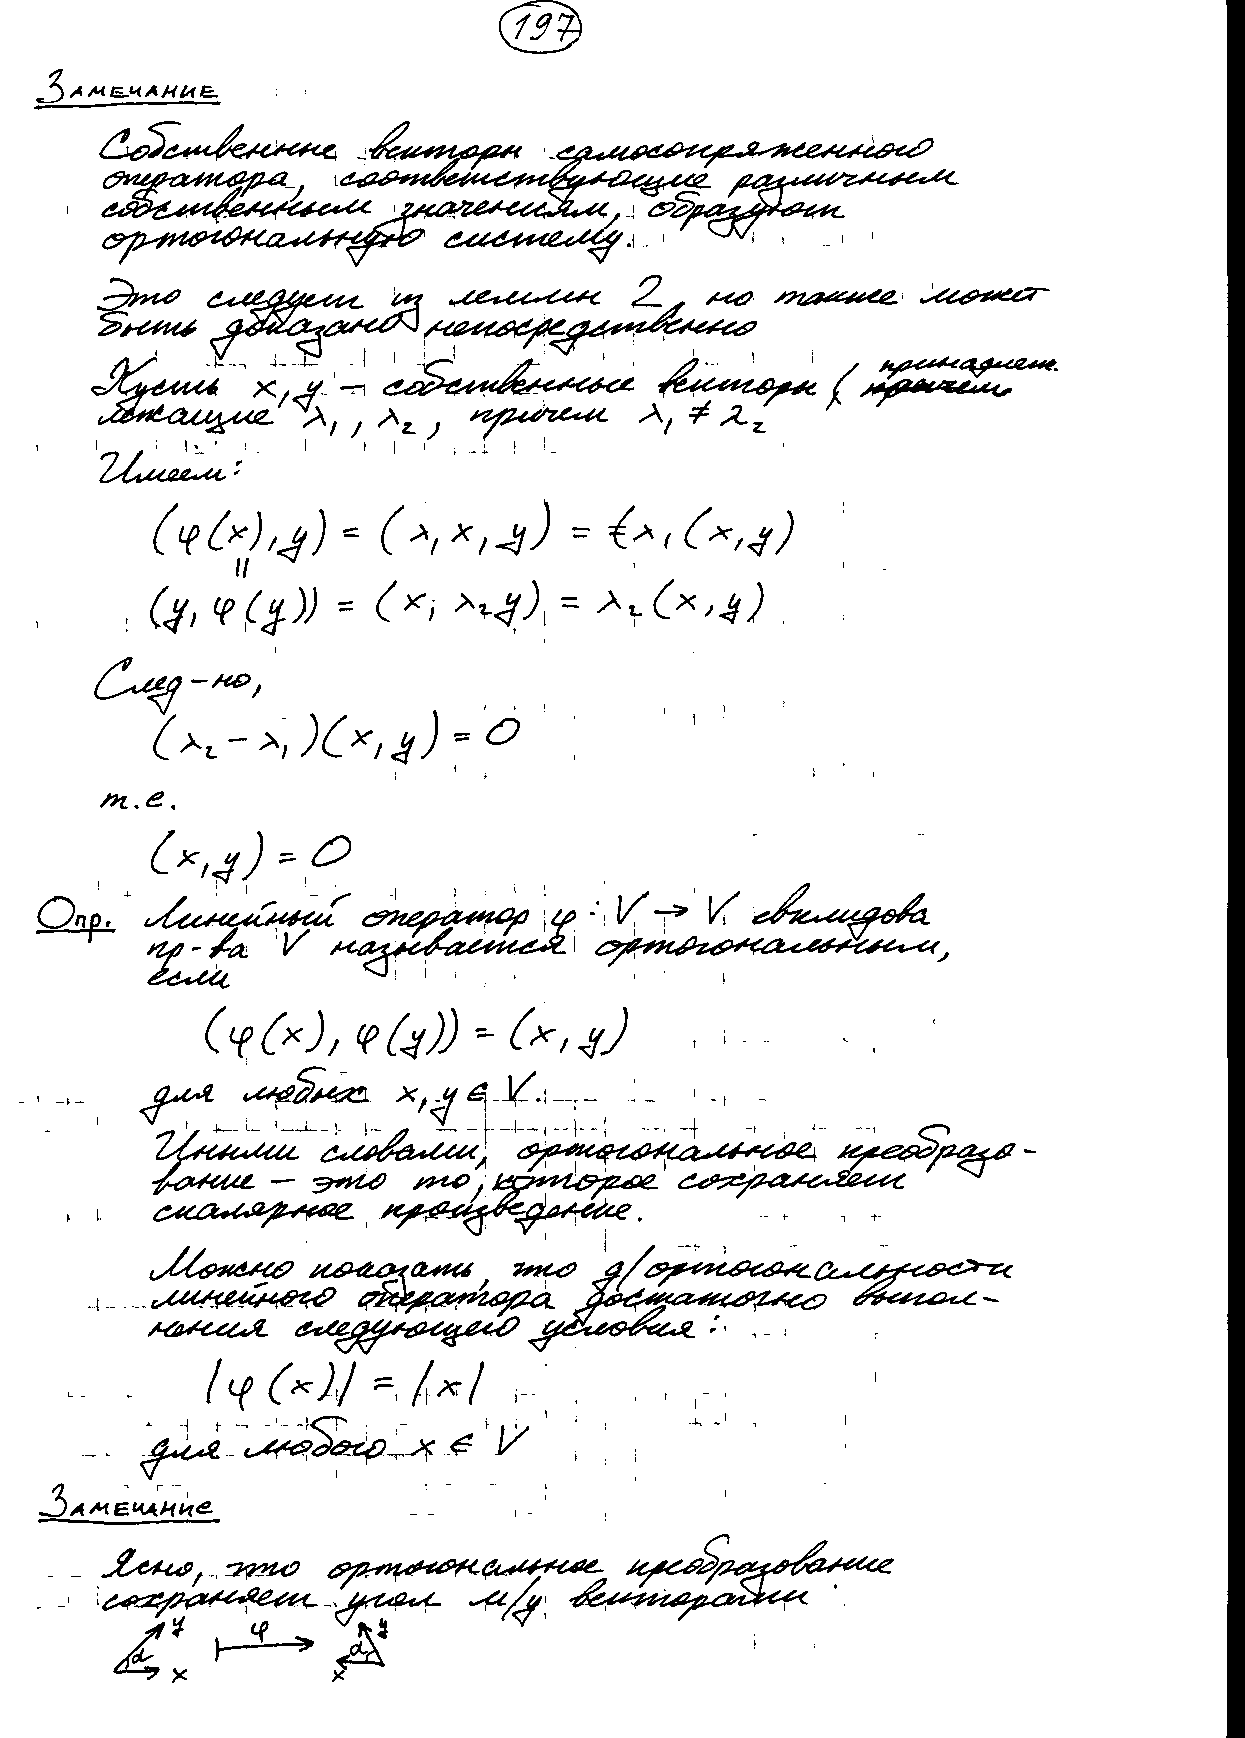
\includepdf[pages=-]{pdf/15_2.pdf}

\subsection{16. Длина вектора, угол между векторами, угол между вектором и подпространством, объём параллелепипеда в евклидовом пространстве.}
\label{sec:orgb8259c6}
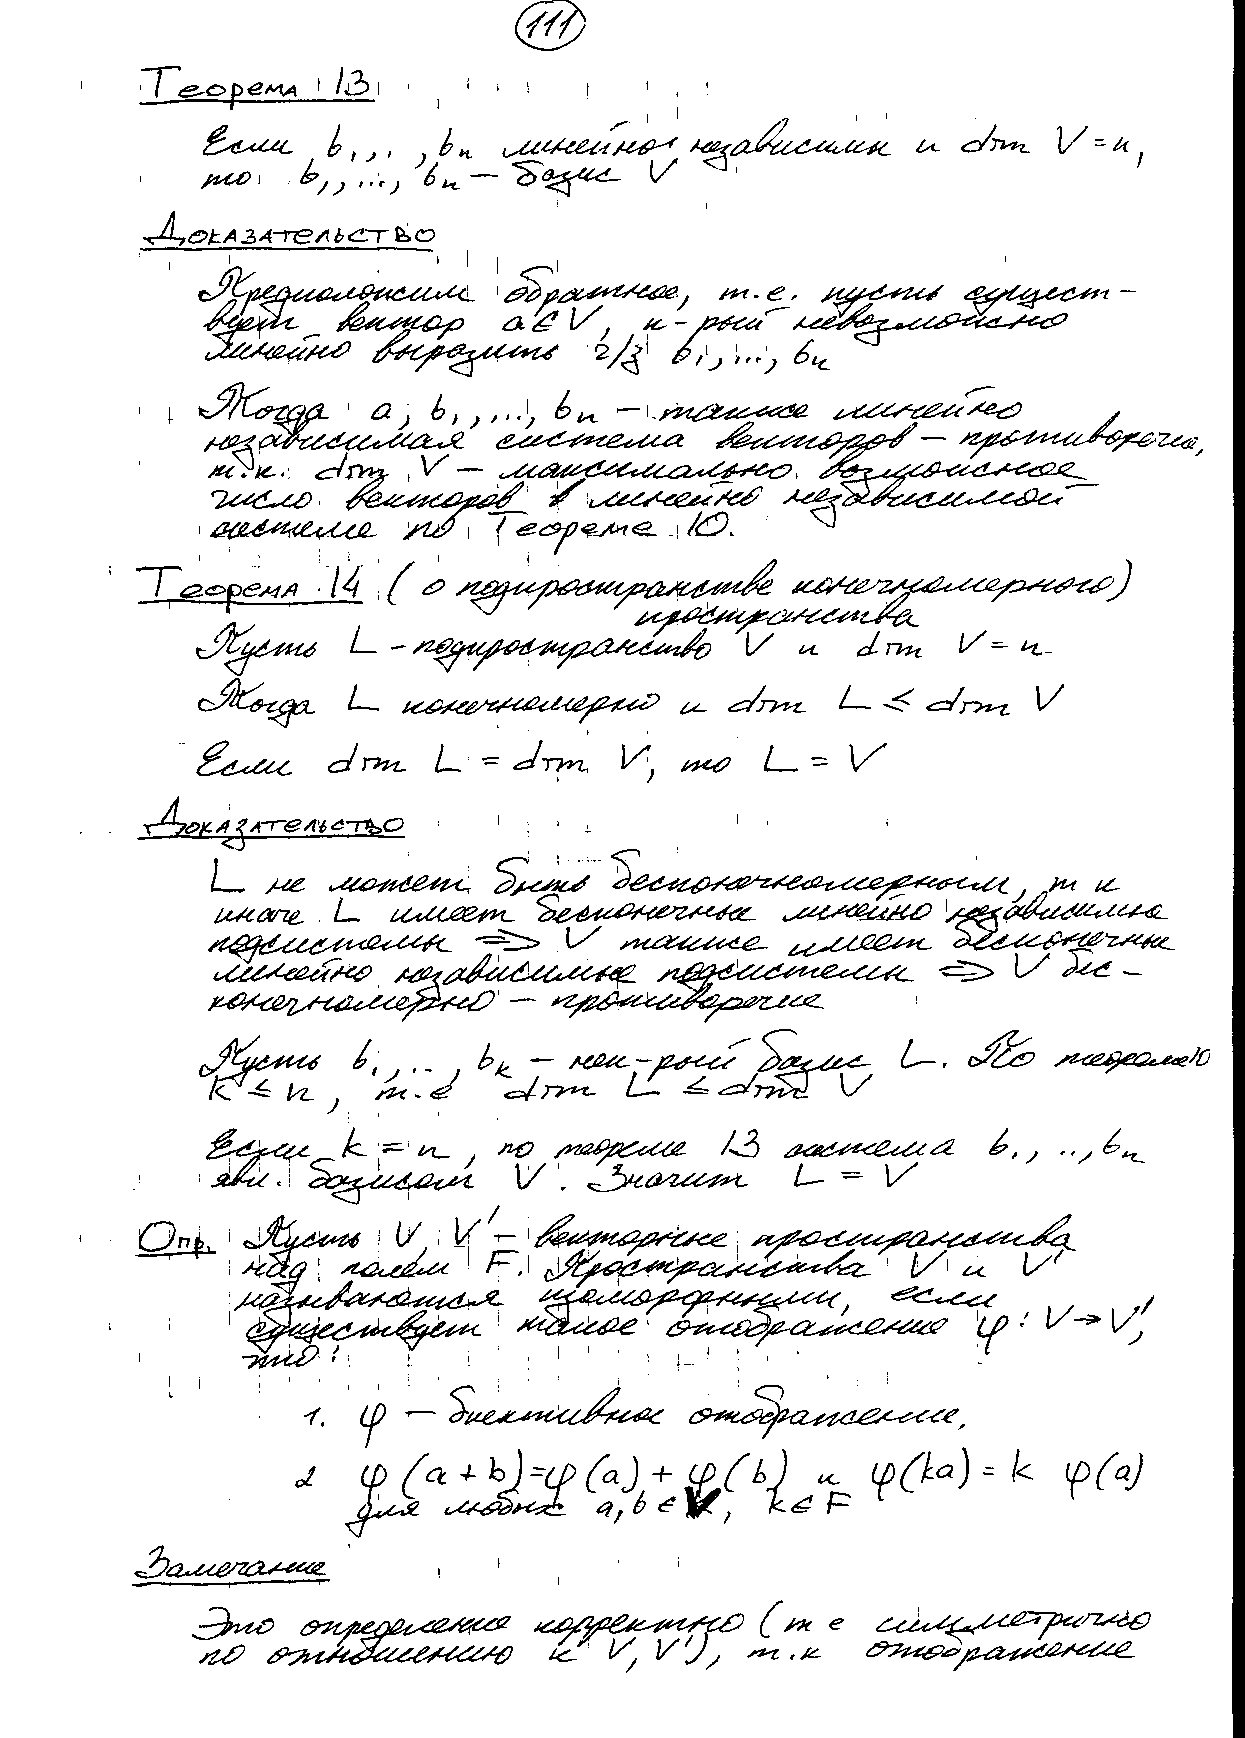
\includepdf[pages=-]{pdf/16_1.pdf}

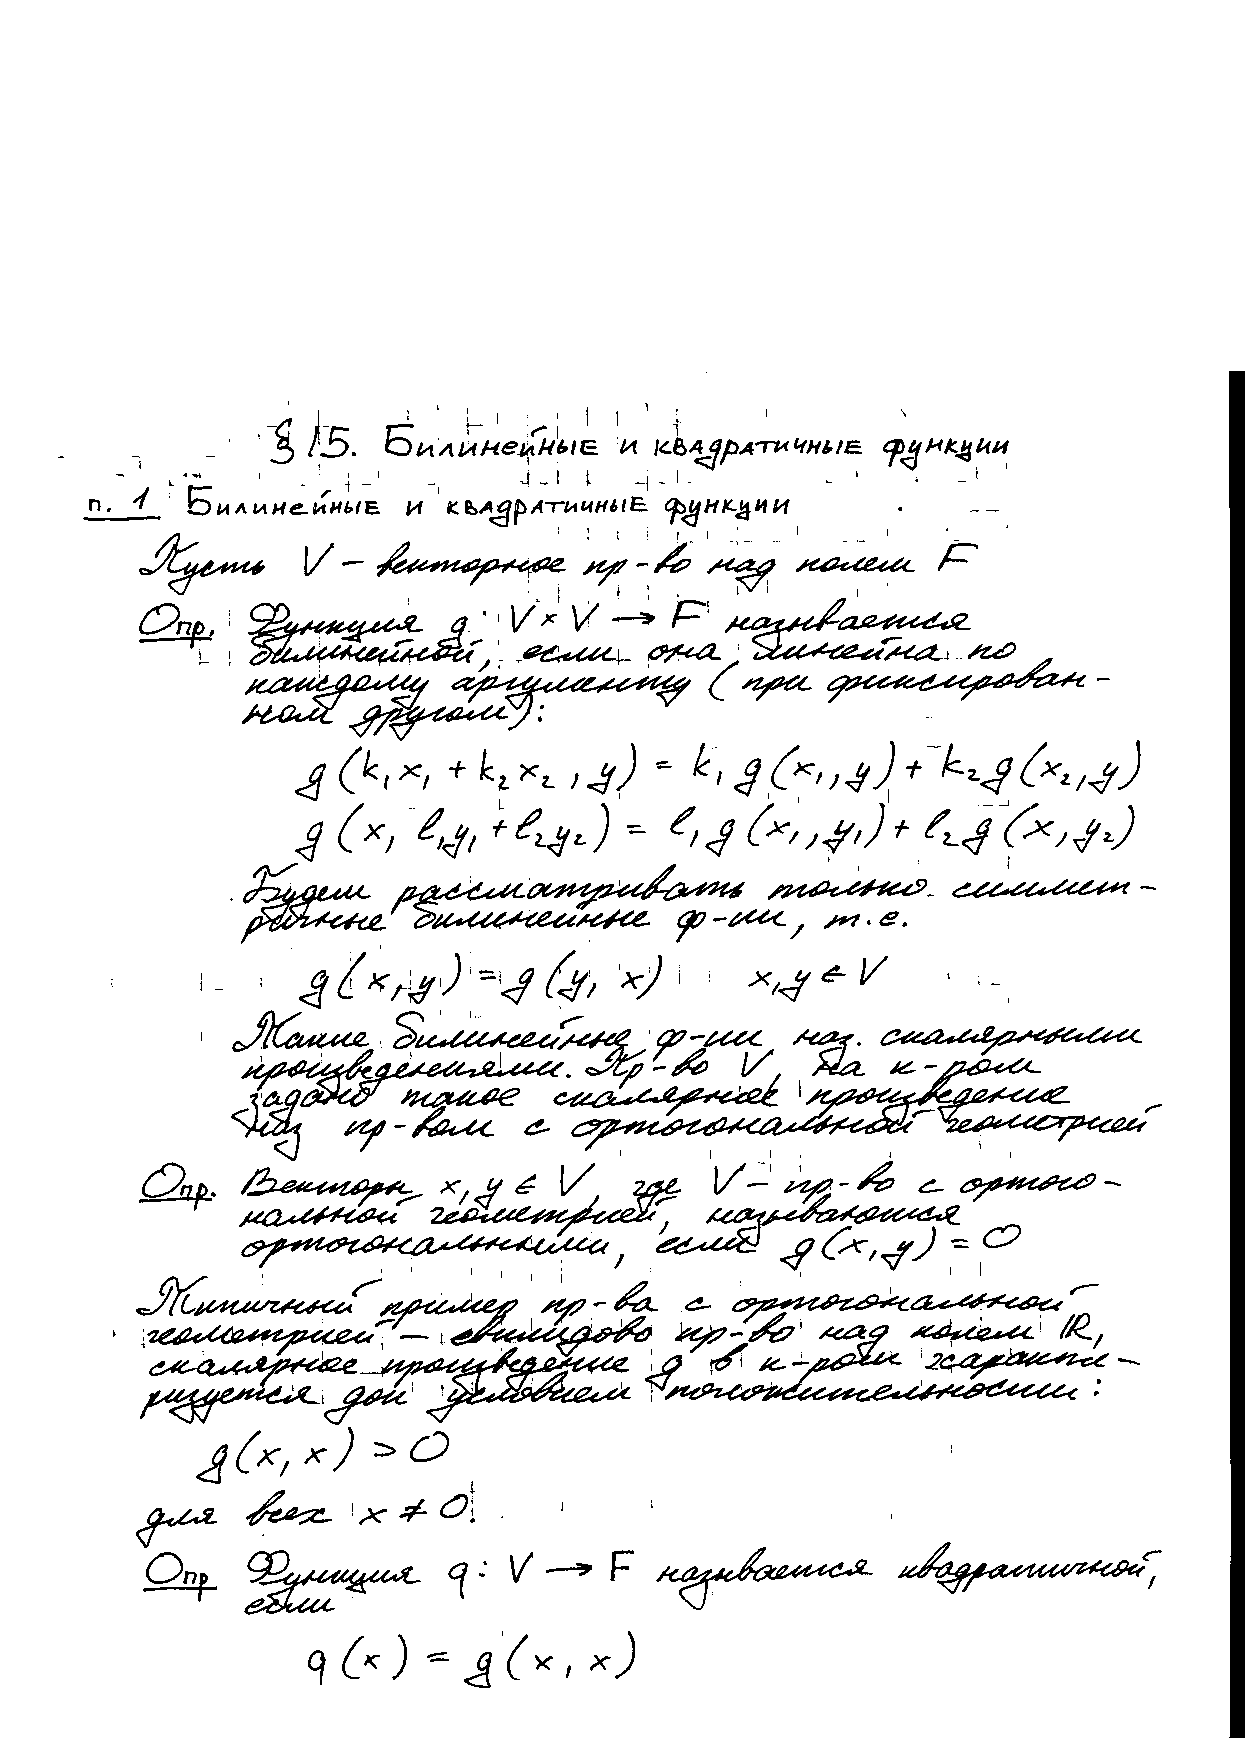
\includepdf[pages=-]{pdf/16_2.pdf}

\subsection{17. Линейный оператор в векторном пространстве. Матрица линейного оператора в данном базисе и её изменение при переходе к другому базису.}
\label{sec:orgccb5490}
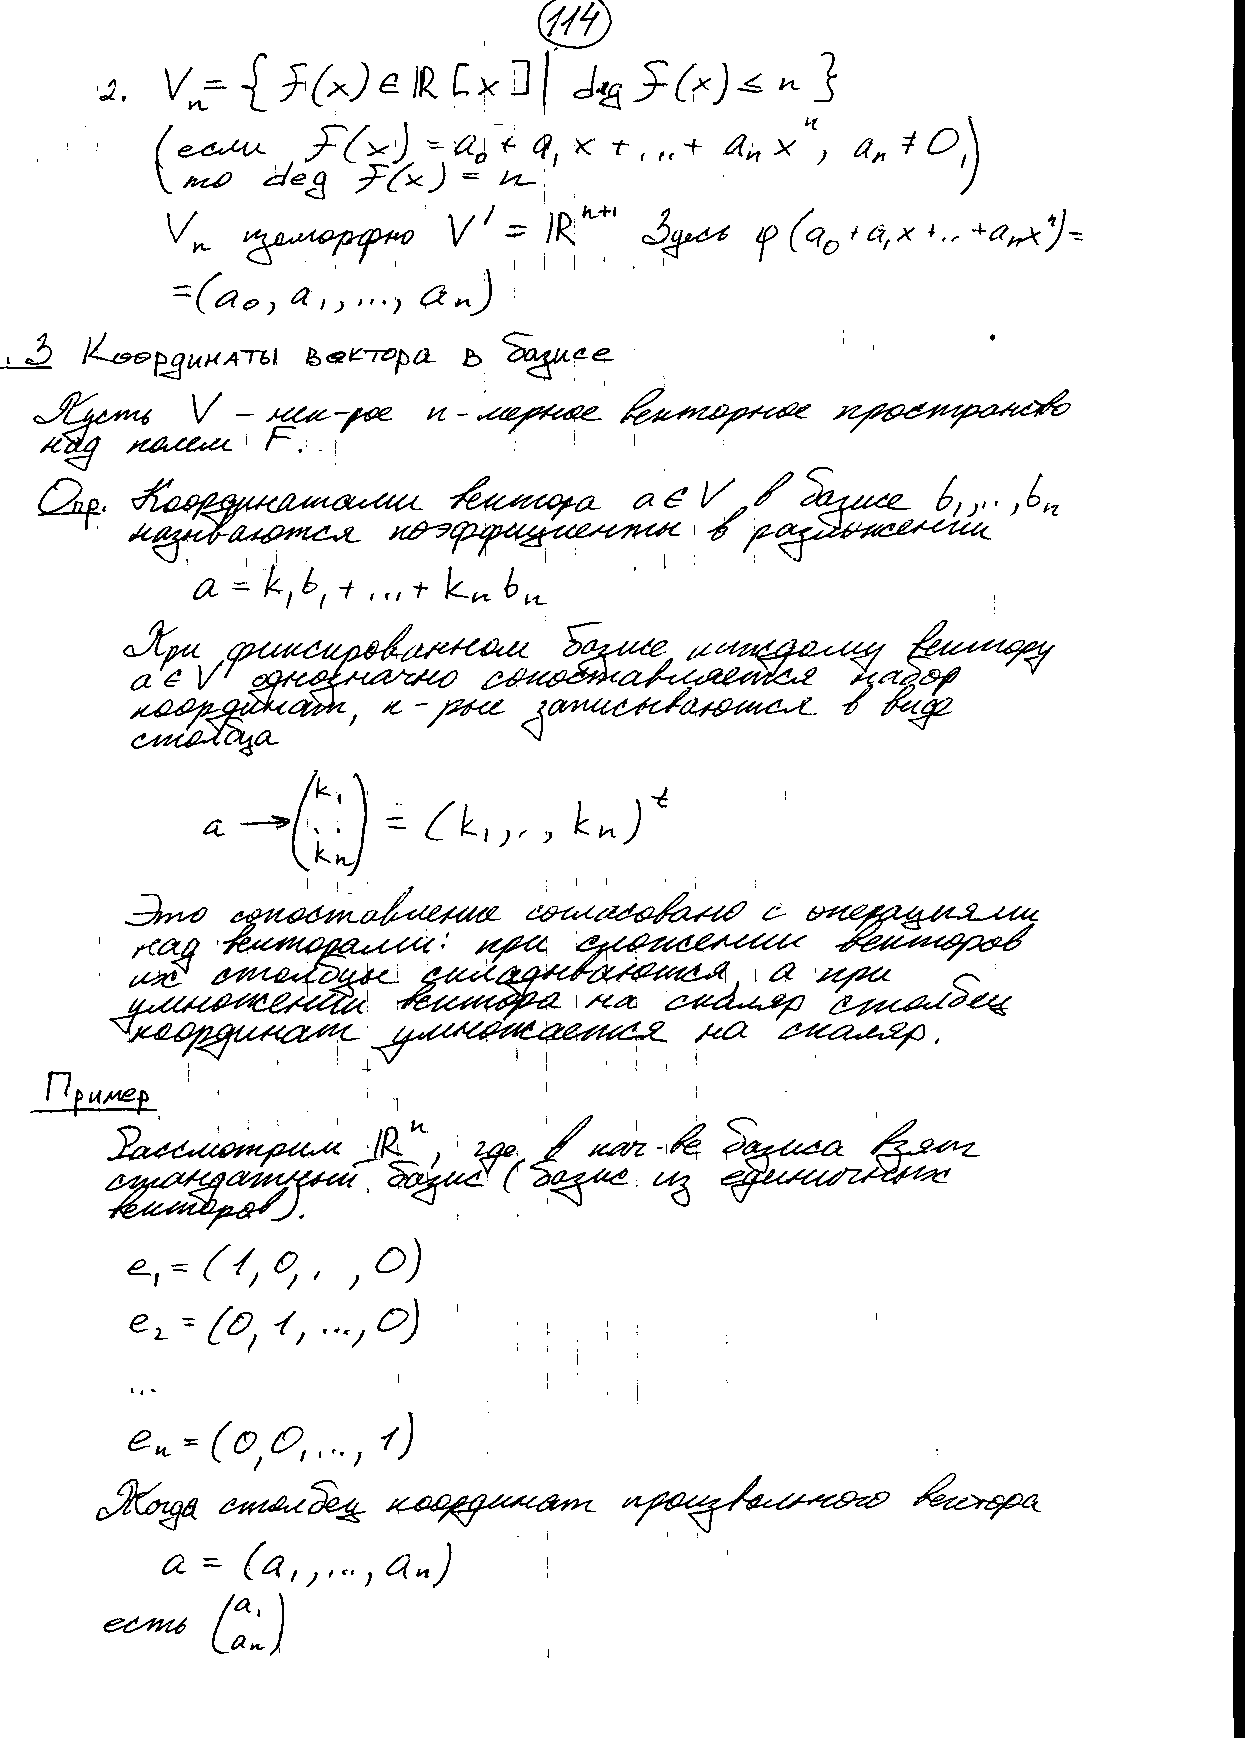
\includepdf[pages=-]{pdf/17_1.pdf}

\includepdf[pages=-]{pdf/17_2.pdf}

\subsection{18. Ядро и образ линейного отображения. Невырожденные линейные операторы.}
\label{sec:orge2b664c}
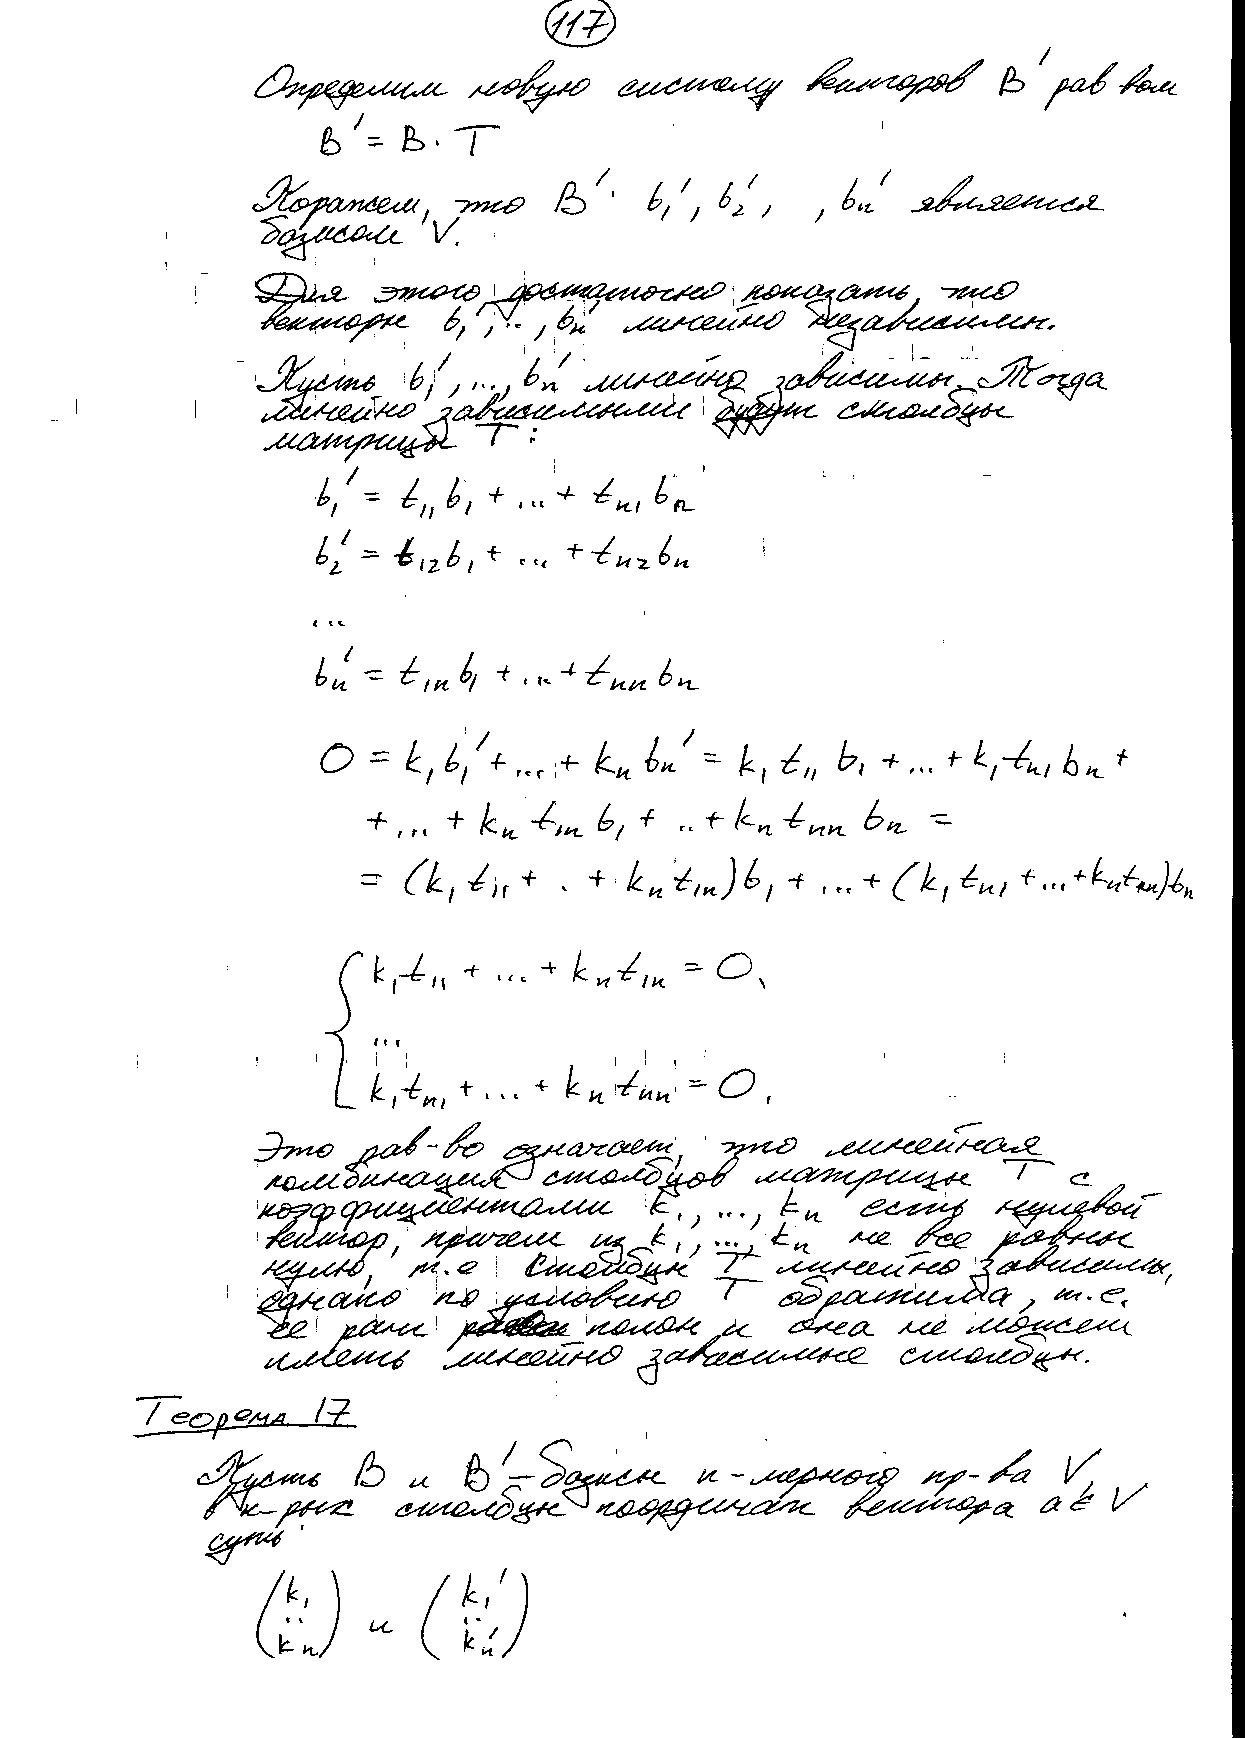
\includepdf[pages=-]{pdf/18_1.pdf}

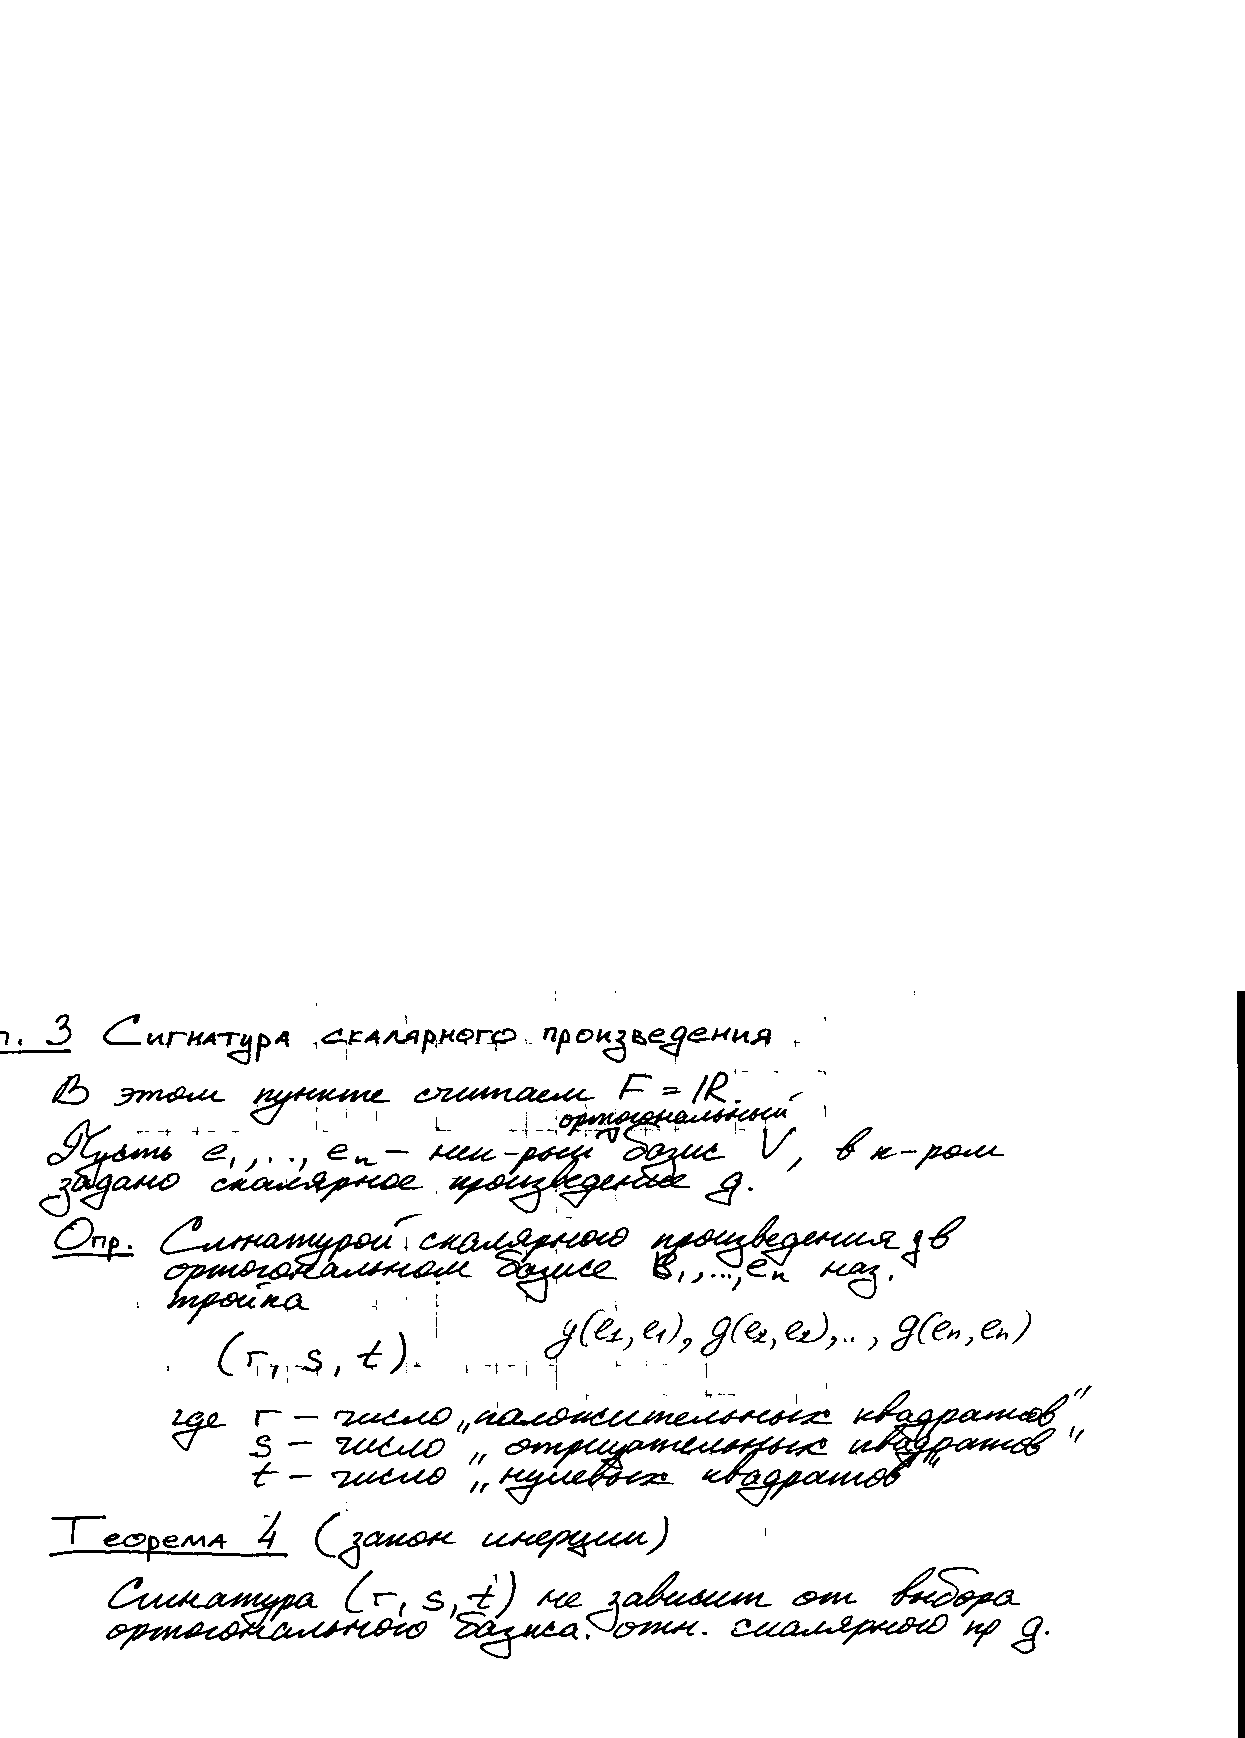
\includepdf[pages=-]{pdf/18_2.pdf}

\subsection{19. Собственные значения и собственные векторы линейного оператора. Характеристический многочлен линейного оператора.}
\label{sec:org1d2b264}
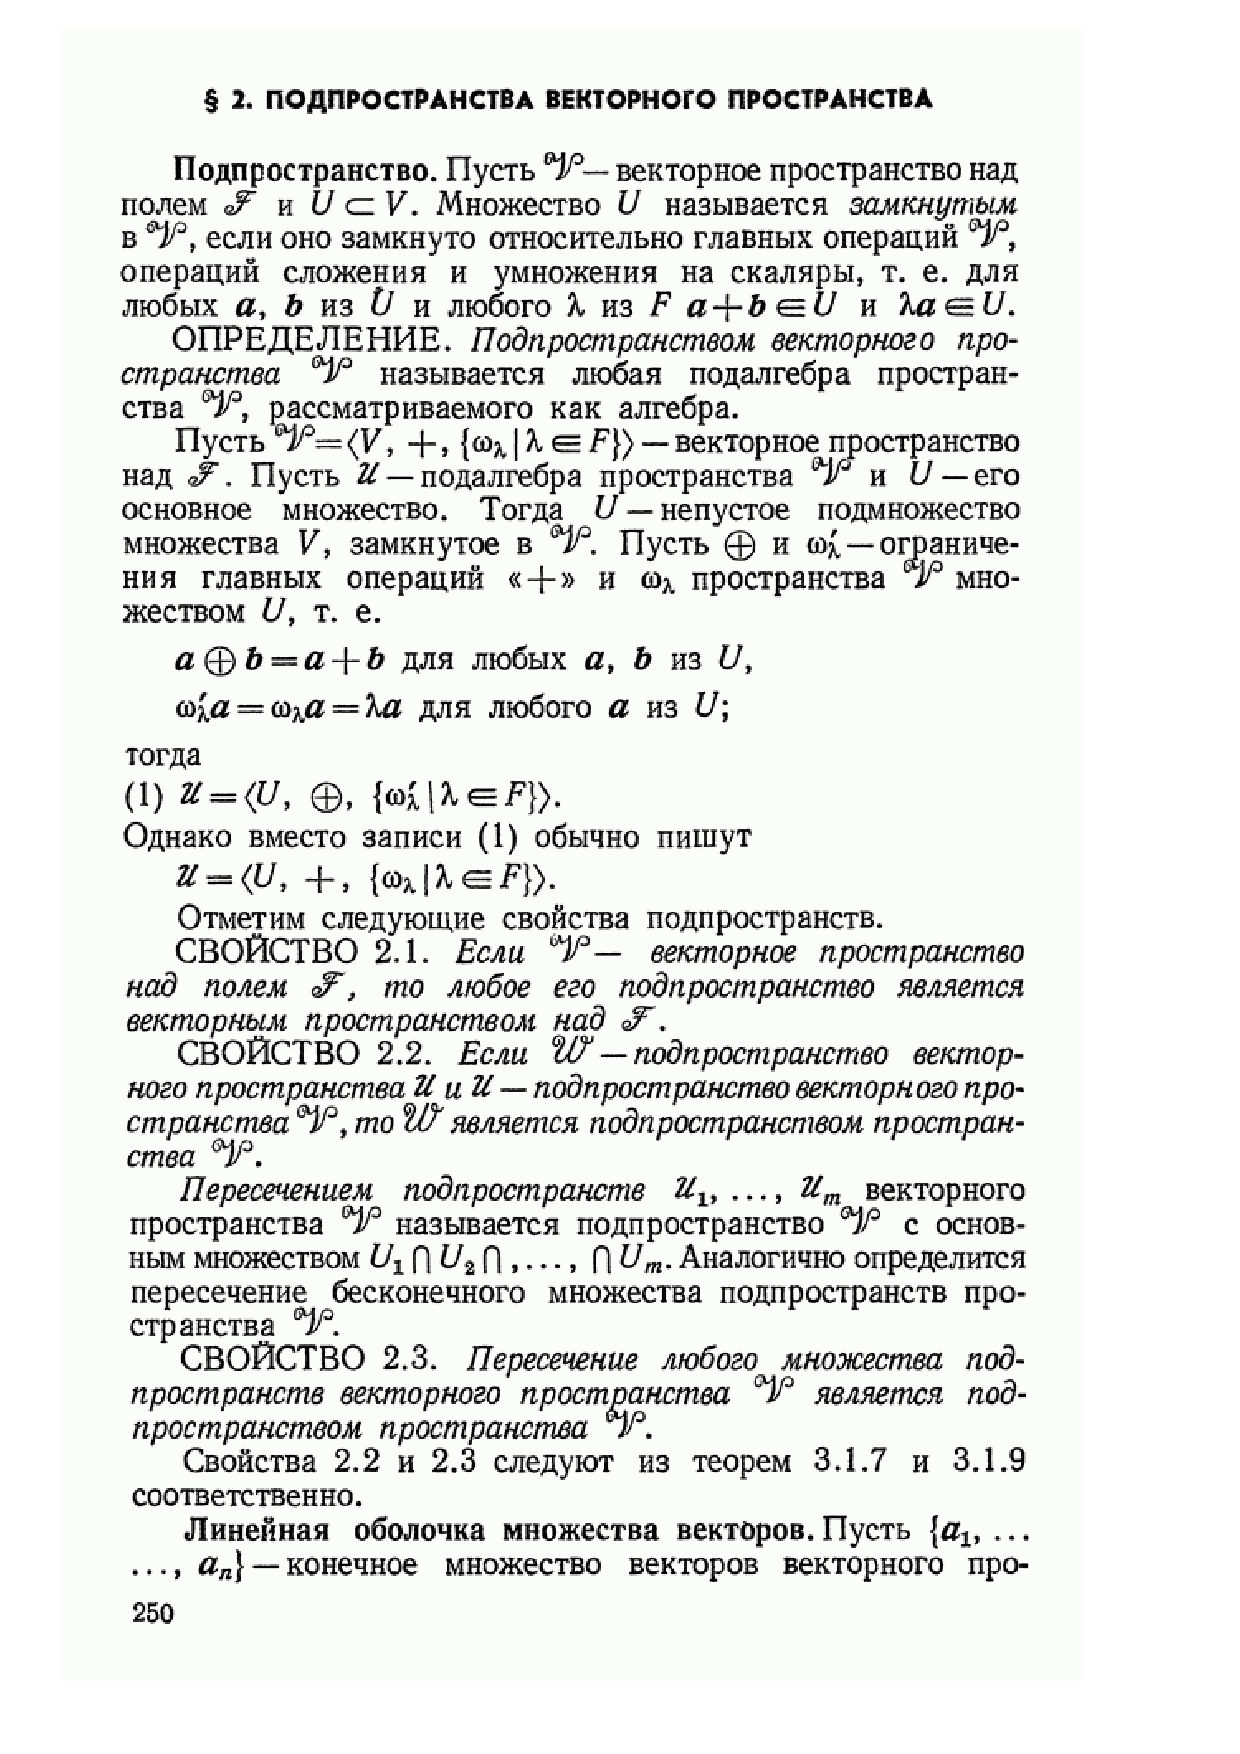
\includepdf[pages=-]{pdf/19_1.pdf}

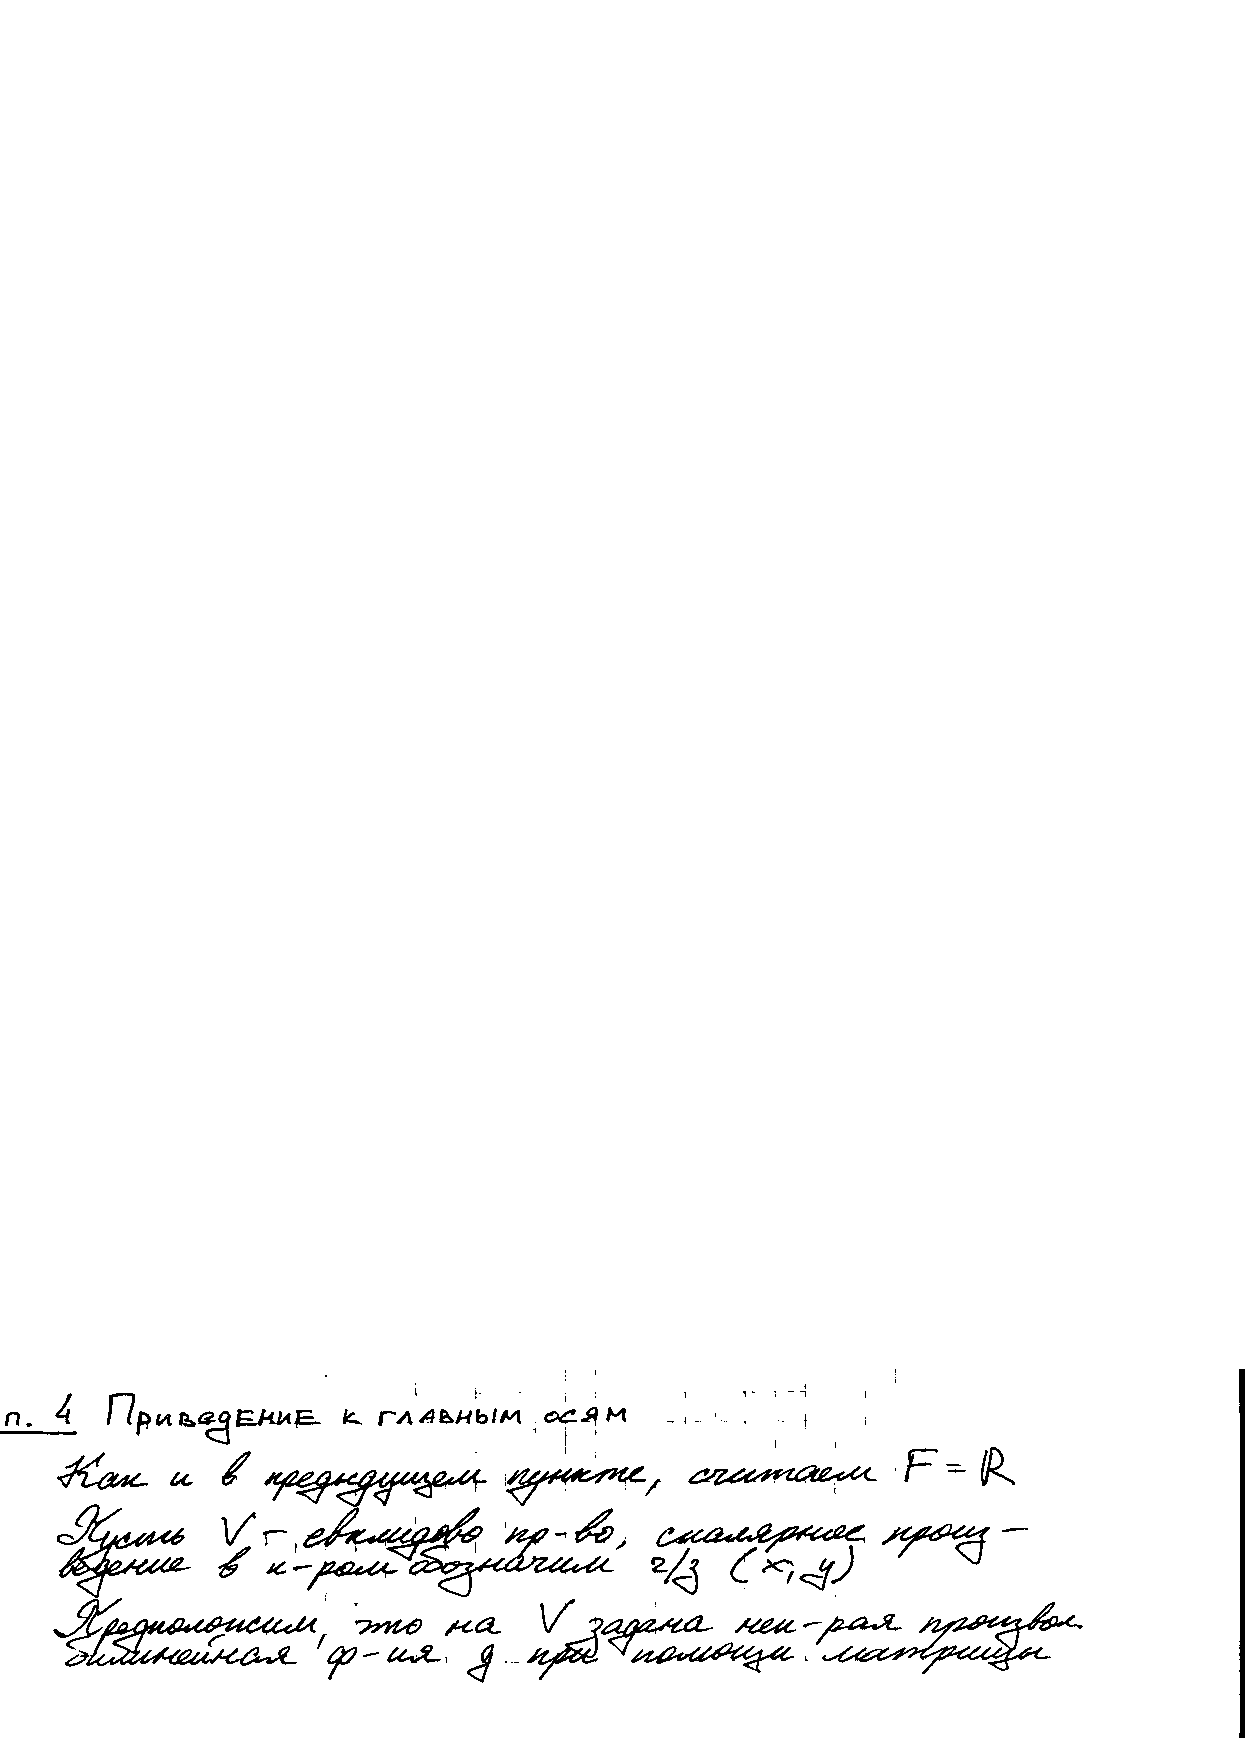
\includepdf[pages=-]{pdf/19_2.pdf}

\subsection{20. Линейная независимость собственных векторов, принадлежащих попарно различным собственным значениям.}
\label{sec:org512834c}
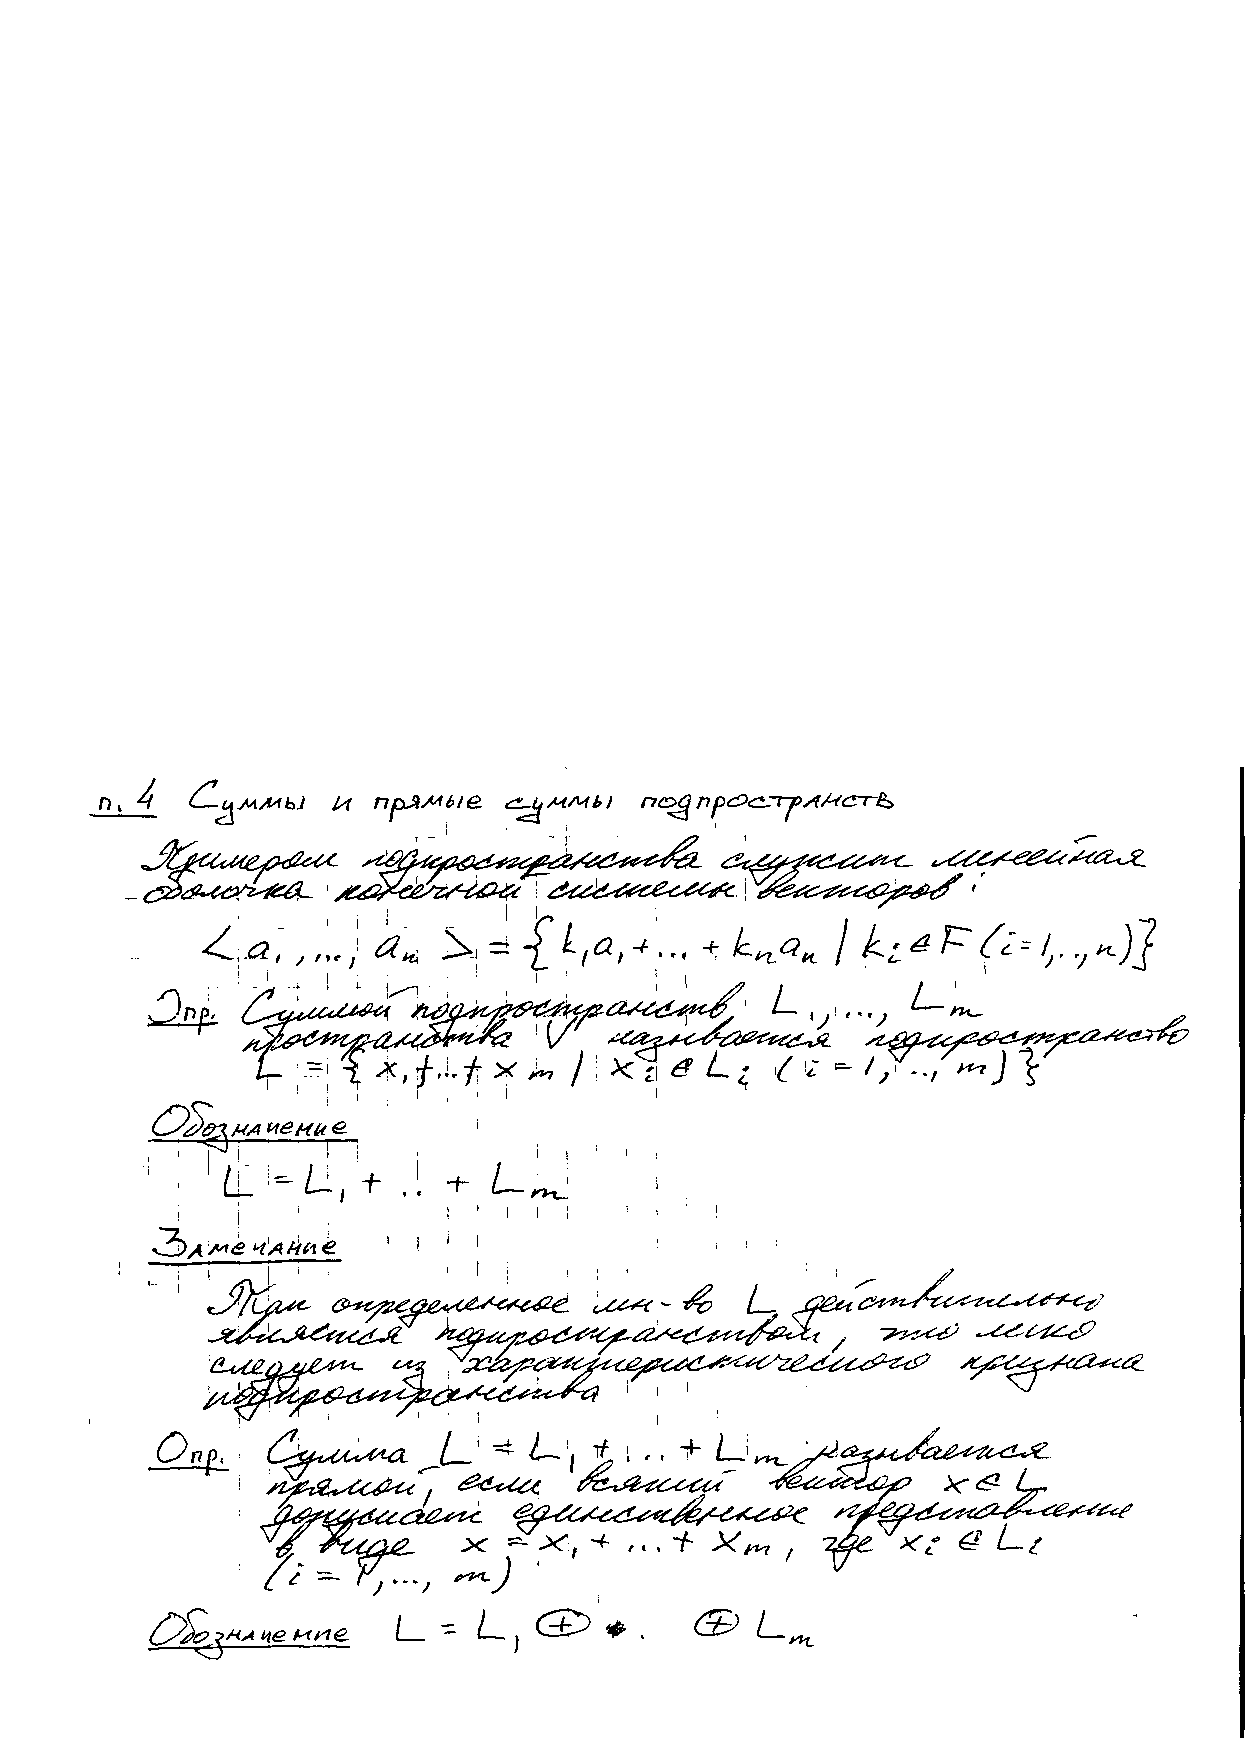
\includepdf[pages=-]{pdf/20_1.pdf}

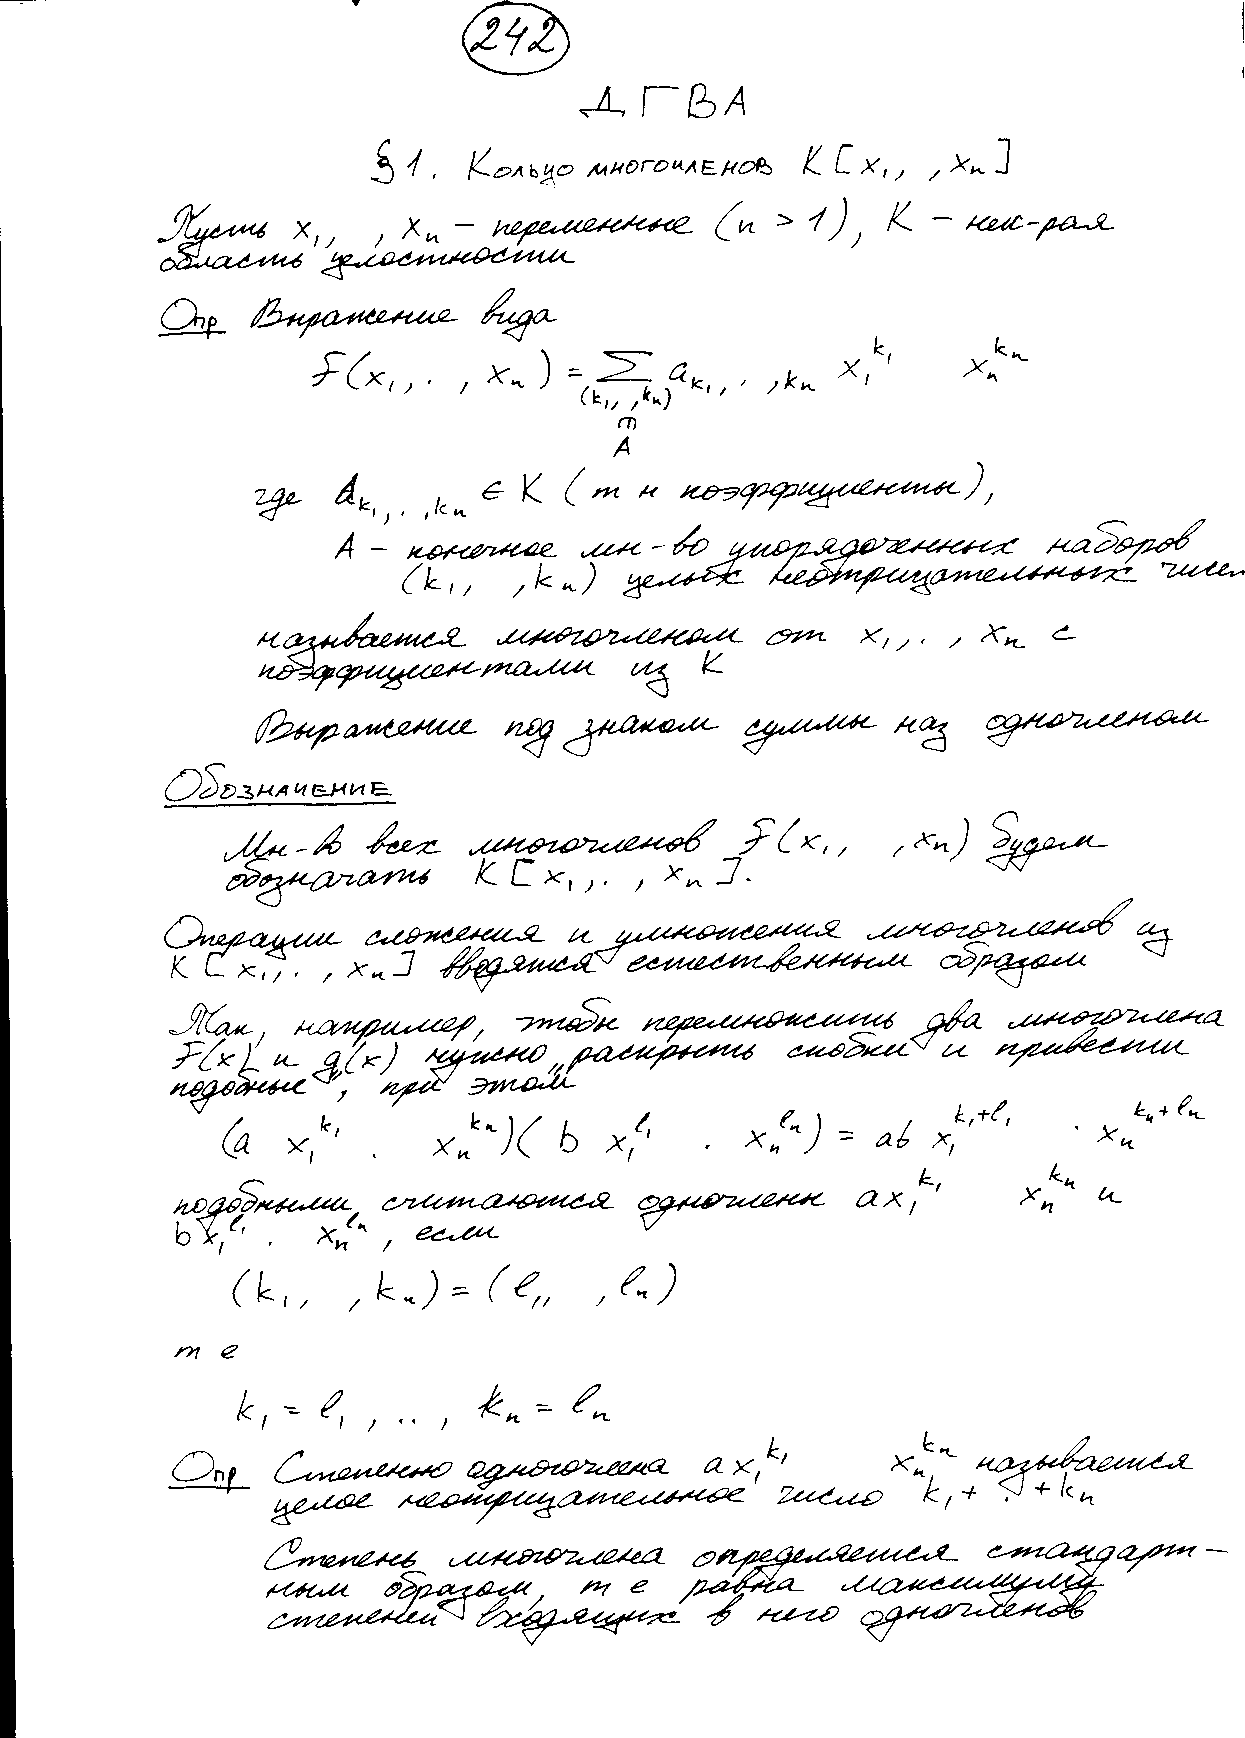
\includepdf[pages=-]{pdf/20_2.pdf}

\subsection{21. Диагонализируемые линейные операторы. Теорема о диагонализируемости линейного оператора с простым спектром. Критерий диагонализируемости.}
\label{sec:org00114bf}
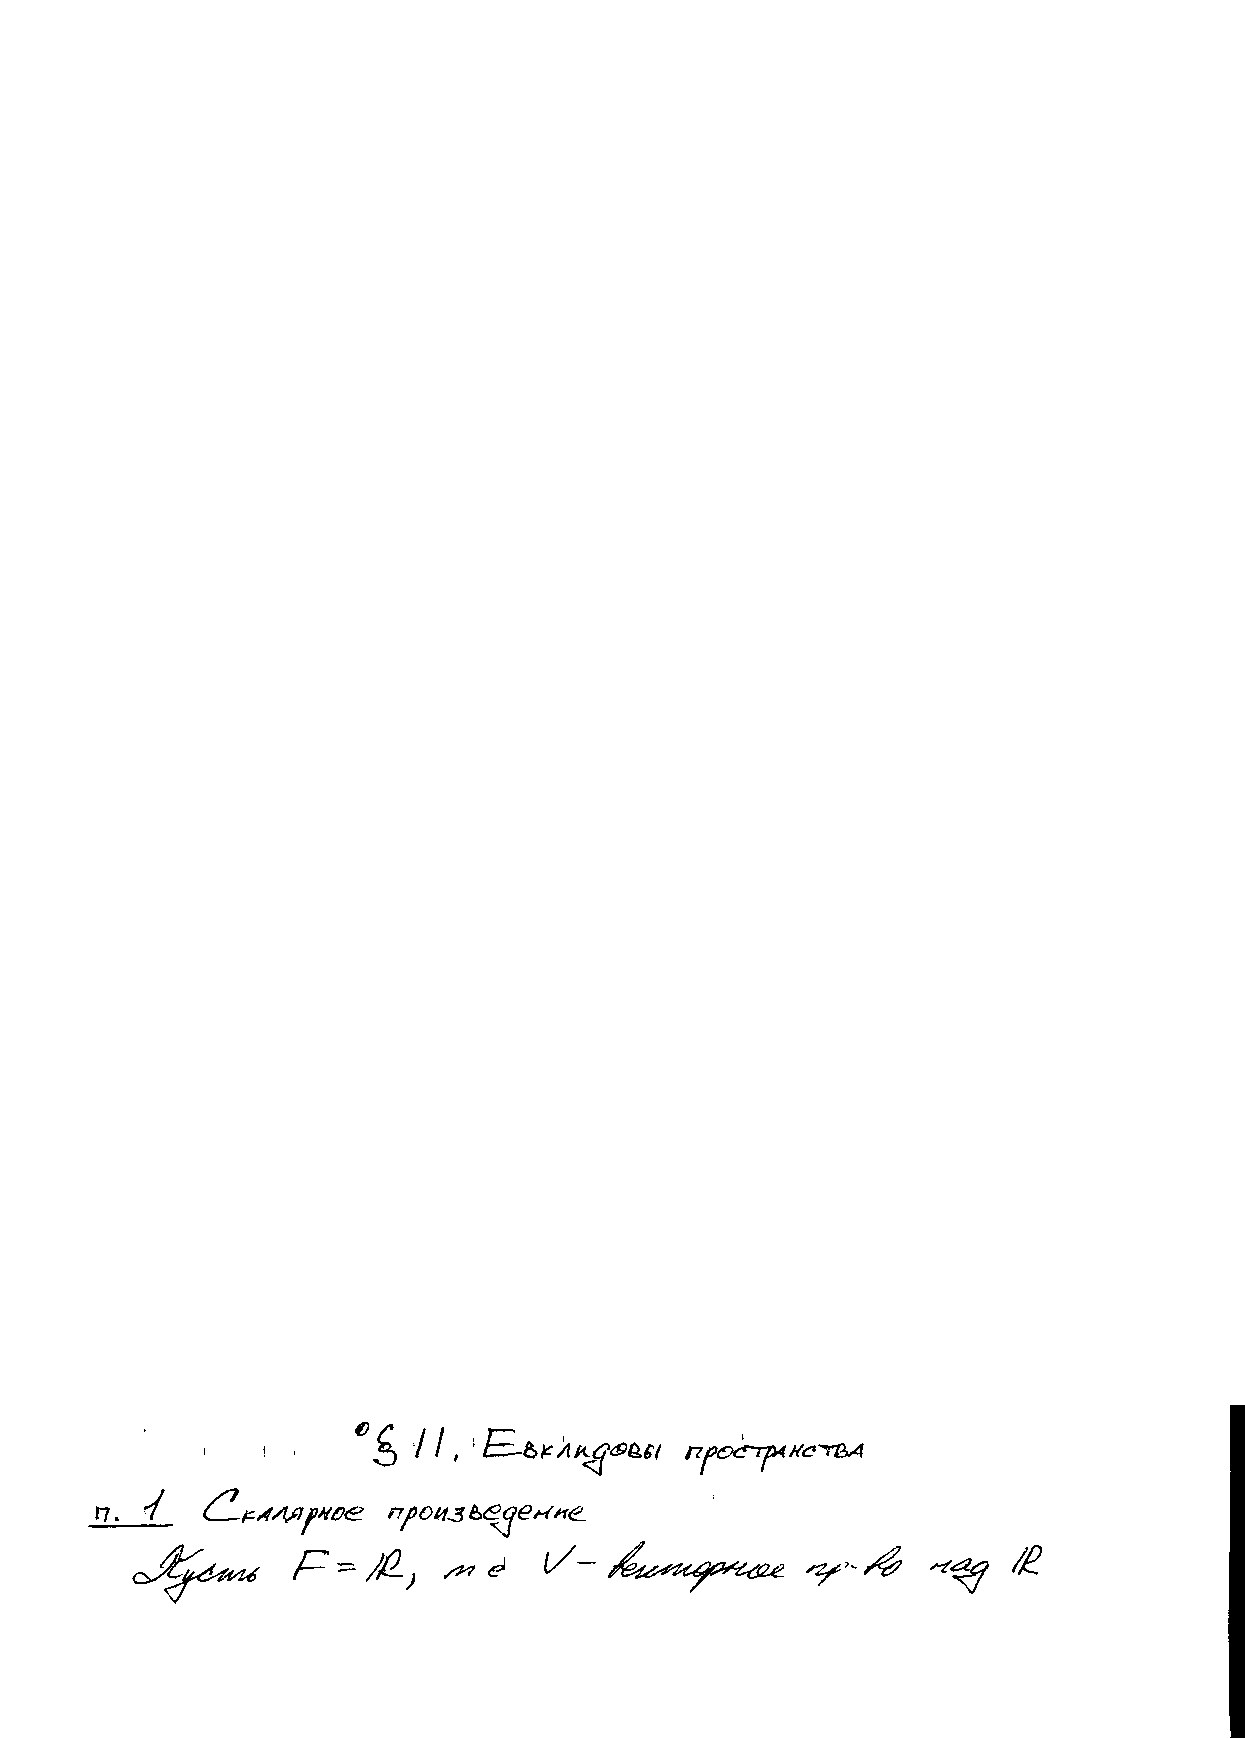
\includepdf[pages=-]{pdf/21_1.pdf}

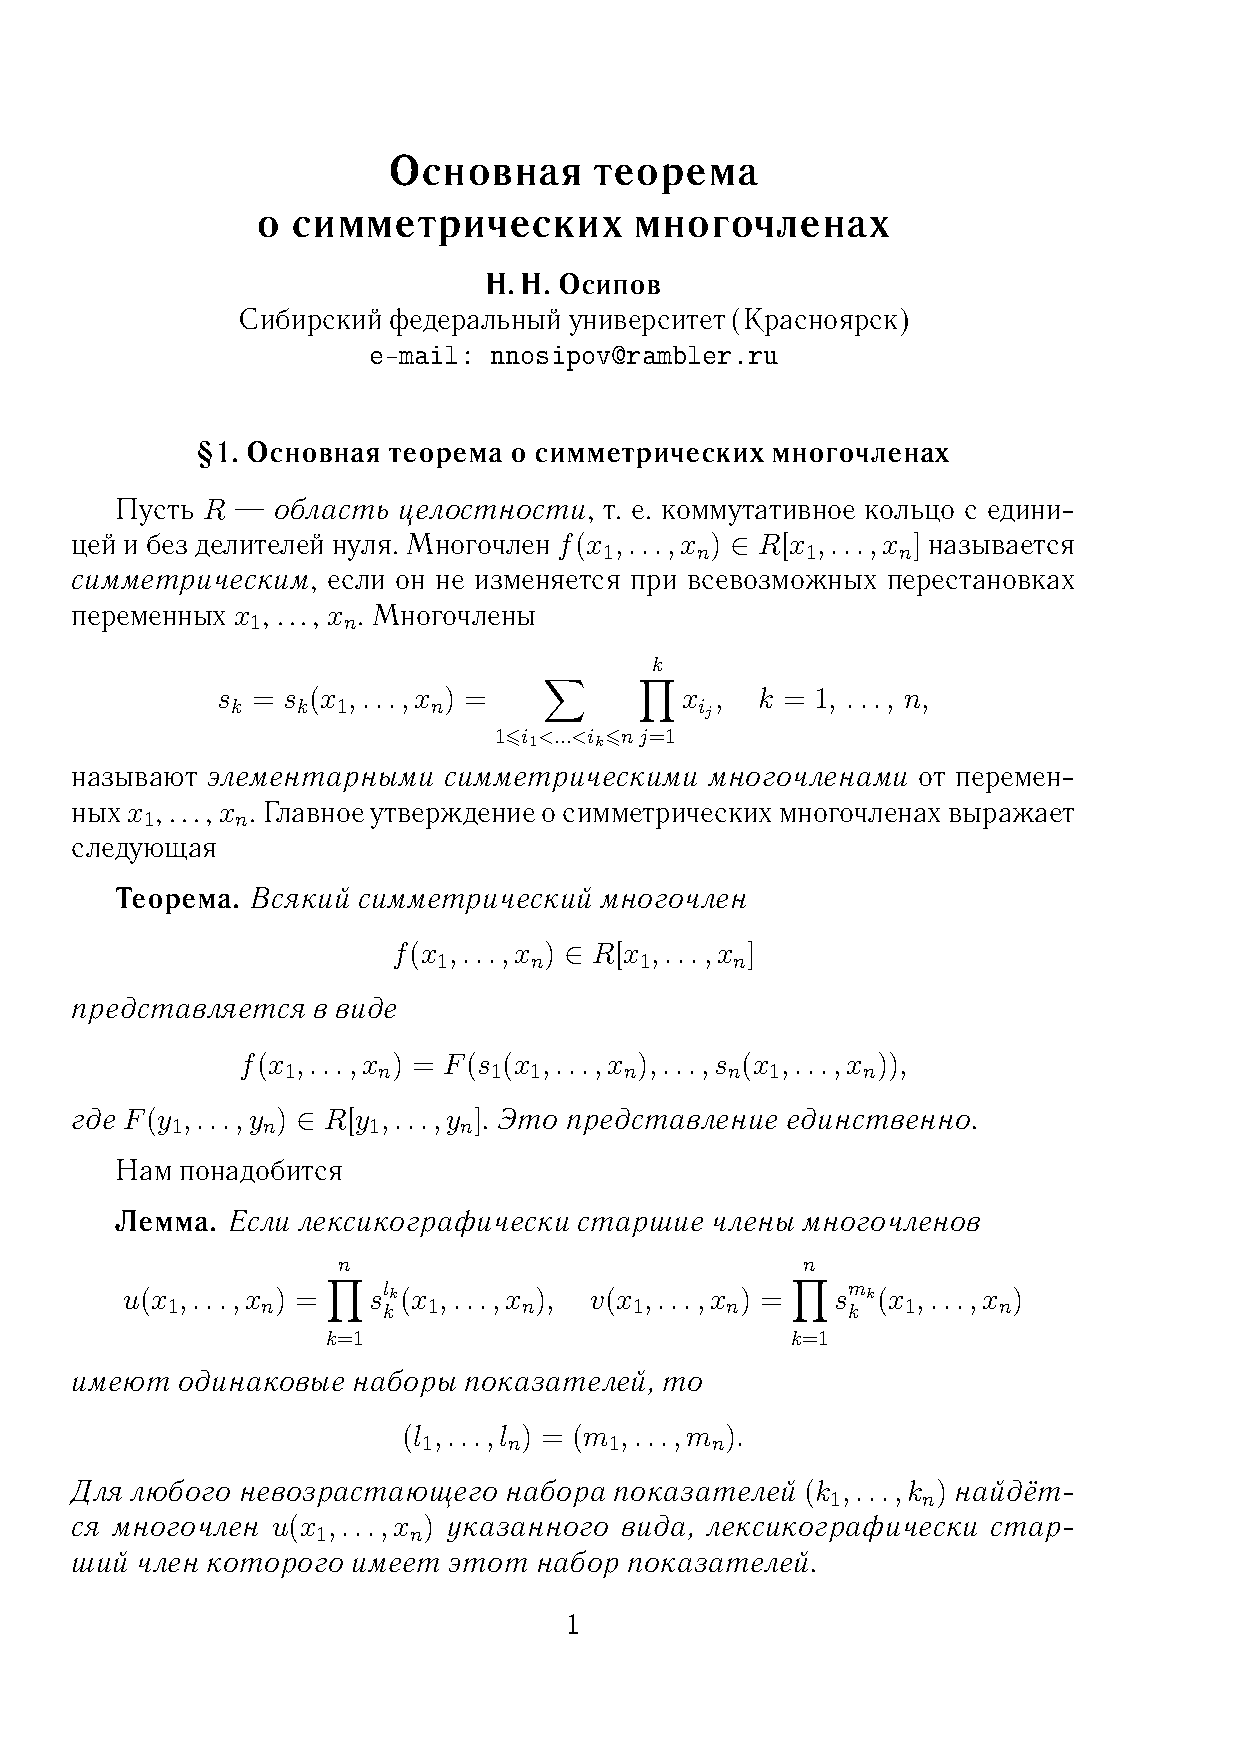
\includepdf[pages=-]{pdf/21_2.pdf}

\subsection{{\bfseries\sffamily TODO} 22. Квадратичные формы. Приведение квадратичной формы к сумме квадратов с коэффициентами методом Лагранжа.}
\label{sec:org8f2625e}
\end{document}
